\documentclass[a4paper, 12pt]{book}
%\usepackage[T1]{fontenc}

\usepackage[a4paper, left=2.5cm, right=2.5cm, top=3cm, bottom=3cm]{geometry}
\usepackage{times}
%\usepackage[latin1]{inputenc}
\usepackage[spanish]{babel} %comentar linea si tu memoria es en ingles.
\selectlanguage{spanish}
\usepackage[utf8]{inputenc}
\usepackage{url}
%\usepackage[dvipdfm]{graphicx}
\usepackage{graphicx}
\usepackage{float} %% H para posicionar figuras
\usepackage[nottoc, notlot, notlof, notindex]{tocbibind} %% Opciones de indice.
\usepackage{latexsym} %% Logo de LaTeX
\usepackage{multirow} %% Para las tablas
\usepackage{pdfpages}
\usepackage{listings} %% para el codigo

%\usepackage[table,xcdraw]{xcolor}

\definecolor{codegreen}{rgb}{0,0.6,0}
\definecolor{codegray}{rgb}{0.5,0.5,0.5}
\definecolor{codepurple}{rgb}{0.58,0,0.82}
\definecolor{backcolour}{rgb}{0.95,0.95,0.92}
\definecolor{darkgray}{rgb}{.4,.4,.4}
\definecolor{purple}{rgb}{0.65, 0.12, 0.82}
\colorlet{punct}{red!60!black}
\definecolor{background}{HTML}{EEEEEE}
\definecolor{delim}{RGB}{20,105,176}
\colorlet{numb}{magenta!60!black}


\lstdefinelanguage{JavaScript}{
	keywords={break, case, catch, continue, debugger, default, delete, do, else, false, finally, for, function, if, in, instanceof, new, null, return, switch, this, throw, true, try, typeof, var, void, while, with, let, const, exports},
	morecomment=[l]{//},
	morecomment=[s]{/*}{*/},
	morestring=[b]',
	morestring=[b]",
	ndkeywords={class, export, boolean, throw, implements, import, this},
	keywordstyle=\color{blue}\bfseries,
	ndkeywordstyle=\color{darkgray}\bfseries,
	identifierstyle=\color{black},
	commentstyle=\color{purple}\ttfamily,
	stringstyle=\color{red}\ttfamily,
	sensitive=true
}

\lstdefinelanguage{json}{
	basicstyle=\normalfont\ttfamily,
	numbers=left,
	numberstyle=\scriptsize,
	stepnumber=1,
	numbersep=8pt,
	showstringspaces=false,
	breaklines=true,
	frame=lines,
	backgroundcolor=\color{background},
	literate=
	*{0}{{{\color{numb}0}}}{1}
	{1}{{{\color{numb}1}}}{1}
	{2}{{{\color{numb}2}}}{1}
	{3}{{{\color{numb}3}}}{1}
	{4}{{{\color{numb}4}}}{1}
	{5}{{{\color{numb}5}}}{1}
	{6}{{{\color{numb}6}}}{1}
	{7}{{{\color{numb}7}}}{1}
	{8}{{{\color{numb}8}}}{1}
	{9}{{{\color{numb}9}}}{1}
	{:}{{{\color{punct}{:}}}}{1}
	{,}{{{\color{punct}{,}}}}{1}
	{\{}{{{\color{delim}{\{}}}}{1}
	{\}}{{{\color{delim}{\}}}}}{1}
	{[}{{{\color{delim}{[}}}}{1}
	{]}{{{\color{delim}{]}}}}{1},
}

\lstdefinestyle{mystyle}{
	backgroundcolor=\color{backcolour},   
	commentstyle=\color{codegreen},
	keywordstyle=\color{magenta},
	numberstyle=\tiny\color{codegray},
	stringstyle=\color{codepurple},
	basicstyle=\ttfamily\footnotesize,
	breakatwhitespace=false,         
	breaklines=true,                 
	captionpos=b,                    
	keepspaces=true,                 
	numbers=left,                    
	numbersep=5pt,                  
	showspaces=false,                
	showstringspaces=false,
	showtabs=false,                  
	tabsize=2
}

\lstset{style=mystyle}


\usepackage{amsmath, amsthm, amssymb} %formulas

\title{Memoria del Proyecto}
\author{Nombre del autor}

\renewcommand{\baselinestretch}{1.5} %%Interlineado

\begin{document}

%\renewcommand{\refname}{Bibliografía}  %%Renombrado
\renewcommand{\appendixname}{Apéndice}

%%%%%%%%%%%%%%%%%%%%%%%%%%%%%%%%%%%%%%%%%%%%%%%%%%%%%%%%%%%%%%%%%%
% PORTADA

\begin{titlepage}
\begin{center}
\begin{tabular}[c]{c c}


\includegraphics[scale=0.25]{img/logo_vect.png}&
\begin{tabular}[b]{l}
\Huge
\textsf{UNIVERSIDAD}  \\
\Huge
\textsf{REY JUAN CARLOS} \\
\end{tabular}
\\
\end{tabular}

\vspace{3cm}

\large
GRADO EN INGENIERÍA DE SISTEMAS AUDIOVISUALES Y MULTIMEDIA

\vspace{0.4CM}

\large
Curso Académico 2019/2020

\vspace{0.8cm}
Trabajo Fin de Grado

\vspace{2.5cm}

\large
MÓDULO DE VISUALIZACIÓN DE DATOS EN REALIDAD VIRTUAL PARA KIBANA
\vspace{4cm}

\large
Autor: Andrea Villaverde Hernández

Tutor: Dr. Jesús María Gonzalez Barahona
\end{center}
\end{titlepage}

\newpage
\mbox{}
\thispagestyle{empty} % para que no se enumere la página

%%%%%%%%%%%%%%%%%%%%%%%%%%%%%%%%%%%%%%%%%%%%%%%%%%%%%%%%%%%%%%%%%%
% FIRMAS

\clearpage
\pagenumbering{gobble}
\chapter*{}

\vspace{-4cm}
\begin{center}
\large
\textbf{Trabajo Fin de Grado}

\vspace{1cm}
\large
MÓDULO DE VISUALIZACIÓN DE DATOS EN REALIDAD VIRTUAL PARA KIBANA

\vspace{1cm}
\large
\textbf{Autor :} Andrea Villaverde Hernández \\
\textbf{Tutor :} Dr. Jesús María Gonzalez Barahona

\end{center}

\vspace{1cm}
La defensa del presente Proyecto Fin de Grado se realizó el día \qquad$\;\,$ de \qquad\qquad\qquad\qquad \newline de 2020, siendo calificada por el siguiente tribunal:

\vspace{0.5cm}
\textbf{Presidente:}

\vspace{1.2cm}
\textbf{Secretario:}

\vspace{1.2cm}
\textbf{Vocal:}

\vspace{1.2cm}
y habiendo obtenido la siguiente calificación:

\vspace{1cm}
\textbf{Calificación:}


\vspace{1cm}
\begin{flushright}
Fuenlabrada, a \qquad$\;\,$ de \qquad\qquad\qquad\qquad de 2020
\end{flushright}

%%%%%%%%%%%%%%%%%%%%%%%%%%%%%%%%%%%%%%%%%%%%%%%%%%%%%%%%%%%%%%%%%
% DEDICATORIA

\chapter*{}
\pagenumbering{Roman} % para comenzar la numeracion de paginas en números romanos.
\begin{flushright}
\textit{Dedicado a \\ 
todos aquellos que \\
nunca se rindieron.}
\end{flushright}

%%%%%%%%%%%%%%%%%%%%%%%%%%%%%%%%%%%%%%%%%%%%%%%%%%%%%%%%%%%%%%%%
% AGRADECIMIENTOS

\chapter*{Agradecimientos}
\markboth{AGRADECIMIENTOS}{AGRADECIMIENTOS} %Encabezado

Ha llegado la hora de cerrar esta etapa y dar un paso hacia nuevas aventuras. Es por eso que quiero hacer una parón, antes de continuar, para agradecer a todas esas personas que me han acompañado en este largo viaje.

Quiero empezar por dar gracias a mi familia, en especial a mis padres. Por la educación que me dieron, por el esfuerzo que han tenido que hacer para que yo pudiera venir a Madrid y, sobretodo, por enseñarme que por mucho que falle ellos siempre estarán ahí para apoyarme.

Gracias a tí, Guillermo. Sin tí yo no hubiera llegado hasta aquí. A pesar de no habernos conocido en esta aventura universitaria, has tenido que sufrir todo el proceso de este proyecto. Sé que sin tí, seguramente hubiera abandonado antes de conseguirlo. Te quiero y siempre te querré.

No me olvido de mis compañeros y amigos. Ellos han sido mi fuerza para poder continuar día a día tanto dentro como fuera de las aulas. Y, aunque hayamos cogidos camidos separados, siguen dentro de mi corazón.

En especial quisiera agradecer también a mi tutor, Jesús M. Gonzalez Barahona. Gracias a él he vuelto a creer en que existen las segundas oportunidades; y que no importa lo que hayas hecho en el pasado, sino lo que eres capaz de hacer hacer ahora.

Y por último, darte las gracias a tí, querido lector. Gracias por dedicarle tiempo a leer esta memoria que tanto esfuerzo he invertido en escribir. 


\vspace{2cm}
Nunca lo olvides:

\textit{<<If you can dream it, you can do it.>> - Walter Elias Disney}
%%%%%%%%%%%%%%%%%%%%%%%%%%%%%%%%%%%%%%%%%%%%%%%%%%%%%%%%%%%%%%%%
% RESUMEN

\chapter*{Resumen}
\markboth{RESUMEN}{RESUMEN} %Encabezado

Este proyecto tiene como objetivo integrar una colección de visualizaciones de datos, dentro de un entorno de Realidad Virtual, para sistemas complejos de visualización e interacción de datos. Como sistema de visualización se ha utilizado Kibana usando la base de datos Elasticsearch. 

Para dicha integración, se ha desarrollado un plugin que, con la biblioteca adecuada, permite visualizar datos en forma de gráficas y disfrutar una experiencia inmersiva. Este plugin crea diferentes tipos de visualizaciones, de la misma manera en que se crean en Kibana; y permite añadirlas dentro de una dashboard.

Para el desarrollo del mismo, se ha utilizado la biblioteca de BabiaxR desarrollada en Javascript usando el framework A-Frame. Además también se ha utilizado lenguajes de programación web como Javascript, CSS y HTML, pues Kibana así lo requiere.

El plugin ha sido alojado en Github y subido a la comunidad de Kibana para que pueda ser descargado por usuarios que estén interesados y quieran colaborar en su mejora.


%%%%%%%%%%%%%%%%%%%%%%%%%%%%%%%%%%%%%%%%%%%%%%%%%%%%%%%%%%%%%%%%%
% RESUMEN EN INGLÉS

\chapter*{Summary}
\markboth{SUMMARY}{SUMMARy} %Encabezado

The aim of this project is integrating data visualizations inside a VR environment for complex visualization and data interaction systems. We have chosen Kibana as our visualization system, using Elasticsearch database.

In order to achieve this integration, we’ve developed a plugin which allows us to display data in 3D charts inside an immersive experience. This plugin can create several visualization types the same way those visualizations are created in Kibana. Visualizations can be managed using a dashboard.

For the plugin development, we used the BabiaXR library using A-Frame framework. Web development languages such as Javascript, CSS and HTML are required for Kibana.

The plugin is hosted by Github and has been uploaded into Kibana’s community for the purpose that users can contribute with updates and improvements.


%%%%%%%%%%%%%%%%%%%%%%%%%%%%%%%%%%%%%%%%%%%%%%%%%%%%%%%%%%%%%%%%%
% ÍNDICES %
%%%%%%%%%%%%%%%%%%%%%%%%%%%%%%%%%%%%%%%%%%%%%%%%%%%%%%%%%%%%%%%%%

% Lo índices se generan automáticamente
% Solo hay que comentar/descomentar la instrucción de LaTeX.

%%%% Índice de contenidos
\tableofcontents
%%%% Índice de figuras
\cleardoublepage
\listoffigures % lista de figuras




%%%%%%%%%%%%%%%%%%%%%%%%%%%%%%%%%%%%%%%%%%%%%%%%%%%%%%%%%%%%%%%%%
% INTRODUCCION %
%%%%%%%%%%%%%%%%%%%%%%%%%%%%%%%%%%%%%%%%%%%%%%%%%%%%%%%%%%%%%%%%%

\cleardoublepage
\chapter{Introducción}
\label{sec:intro} %etiqueta para referenciar luego ~\ref{sec:intro}
\pagenumbering{arabic} %para empezar enumeracion con numeros

En este capítulo se hará una breve descripción de lo que tratará el proyecto y su motivación. También definiremos cuáles serán los objetivos a cumplir. Por último, se explicará la estructura de esta memoria y se facilitará la distribución del software en caso de consulta. 

\section{Contexto}
\label{sec:contexto}

Actualmente, la gestión de grandes volúmenes de datos está a la orden del día. Empresas e investigadores trabajan constantemente con ellos; pero los seres humanos no somos capaces de procesar tales cantidades de datos. Para solucionar esto se crearon diferentes formas de poder visualizar estos datos, pues nos es más fácil interpretar la información si nos la presentan de manera gráfica. Es por esto que, a día de hoy, se siguen buscando diferentes maneras de representar datos que faciliten esta labor y sean accesibles desde cualquier parte.

Por otra parte, existe otra tecnología que también está en auge: la Realidad Virtual. Esta te permite crear experiencias inmersivas en un entorno 3D. Muchos creen que la Realidad Virtual se utiliza únicamente en la industria del entretenimiento audiovisual o videojuegos; pero su uso llega mucho más allá, pues también se usa como herramientas en educación, medicina, milicia y un gran etcétera que poco a poco va incrementándose.


\section{Motivación}
\label{sec:motivacion}

A primera vista, estas dos tecnologías no tienen nada que ver; pero la cosa cambia si las combinamos. Nuestra motivación para este proyecto es combinar ambas y crear una herramienta que nos permita mostrar cualquier tipo de dato y podamos visualizarlo en una experiencia inmersiva. Dentro de este entorno podremos visualizar dichos datos e interactuar con ellos.

Lo ideal sería que fuera accesible para cualquiera en cualquier parte. Con la llegada de los nuevos dispositivos portátiles se nos facilita la accesibilidad en cualquier parte; pero nos encontramos con la situación de que puede que nuestro dispositivo no sea compatible con el software. Para solucionar este tipo de incompatibilidades se está intentando trasladar estas herramientas al entorno web, pues prácticamente todos los dispositivos son compatibles.

Ya existen herramientas como Freeboard, Many Eyes o Kibana que permiten visualizar datos a través de un navegador web. Para este proyecto utilizaremos Kibana. Esta herramienta permite monitorizar datos que proceden de Elasticsearch.

\begin{figure}[H]
  \centering
      \minipage{0.45\textwidth}
      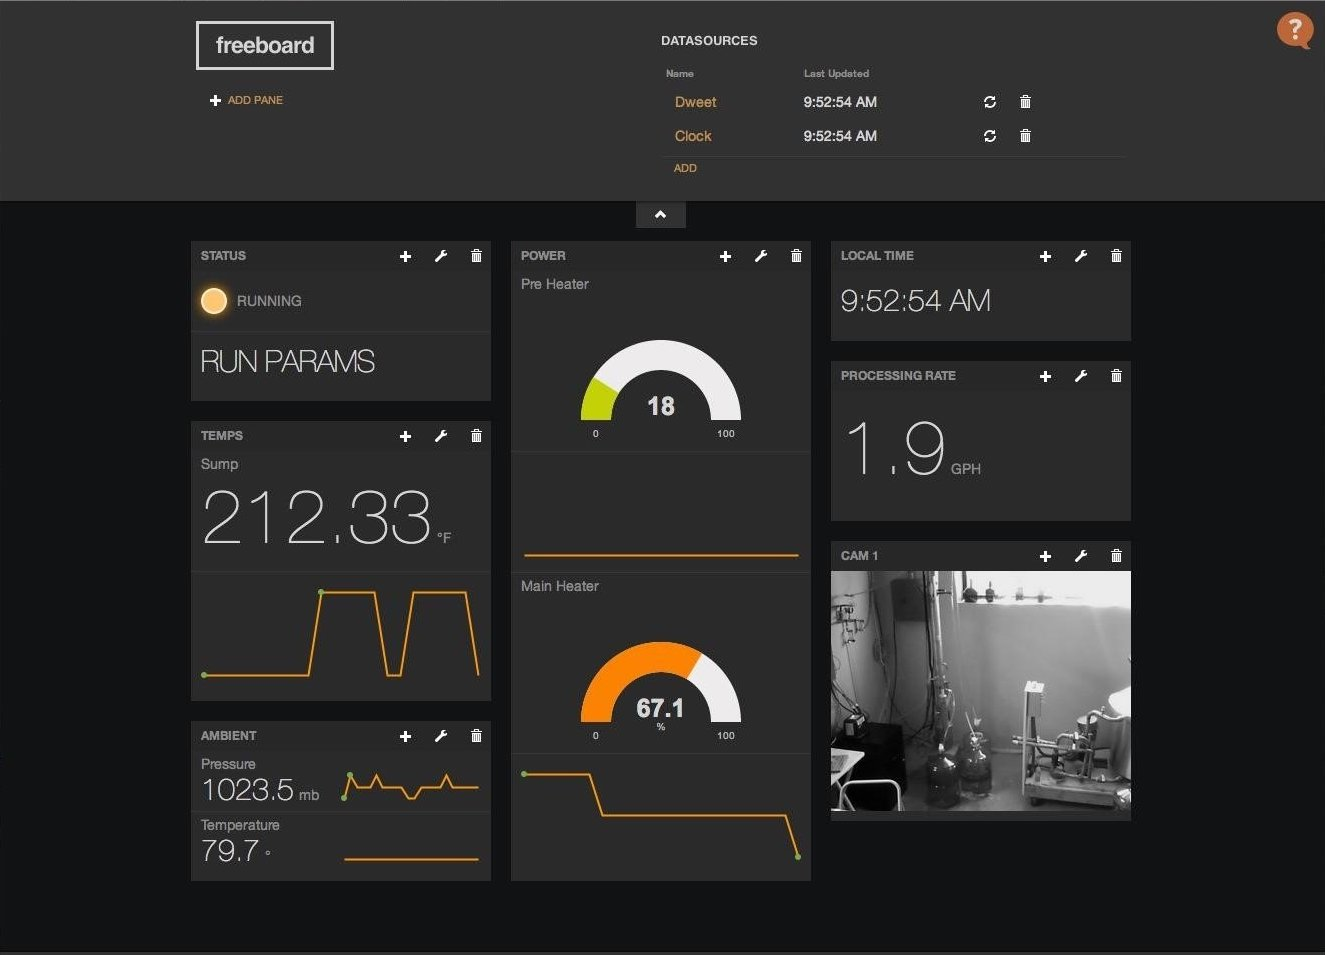
\includegraphics[height=5.5cm, keepaspectratio]{img/development/freeboard.jpg}
      \caption{Freeboard Dashboard}
      \label{fig:freeboard}
      \endminipage\hfill
      \minipage{0.45\textwidth}
      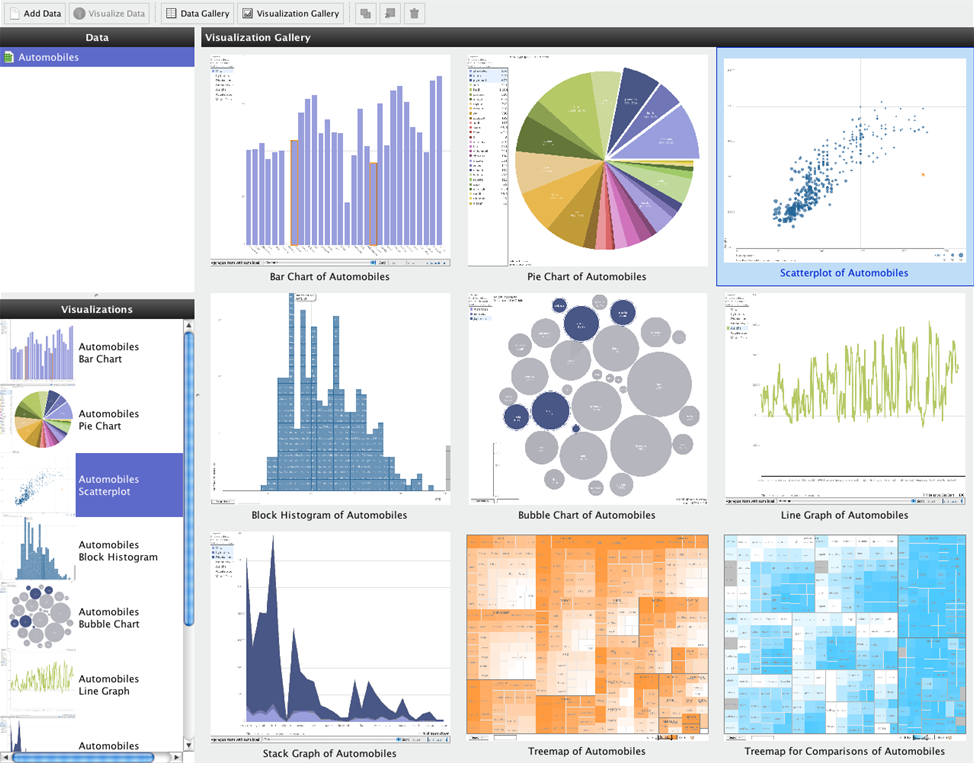
\includegraphics[height=5.5cm, keepaspectratio]{img/development/manyeyes.png}
      \caption{Many Eyes Dashboard}
      \label{fig:manyeyes}
      \endminipage\hfill
\end{figure}


En cuanto a la Realidad Virtual, existe una API experimental en Javascript llamada WebXR la cual proporciona soporte a dispositivos de Realidad Virtual (HTC Vive, Oculus Rift, Google Cardboard, etc) en un navegador web. A raíz de esto se han creado muchos proyectos o frameworks que permiten desarrollar estas experiencias dentro de una página web. En este proyecto trabajaremos con A-Frame y buscaremos componentes de gráficas que se hayan creado con este framework.



\section{Objetivo General}
\label{sec:objetivogeneral}

El objetivo principal de este proyecto es una prueba de concepto de visualización de datos en un entorno de Realidad Virtual. Para ello utilizaremos una herramienta que, a pesar de estar diseñada para crear visualizaciones de datos en un sistema tradicional 2D, permita también representarlos en un sistema 3D simulado en un entorno VR con la posibilidad de inmersión.

En resumen, vamos a crear un plugin de visualización para el software Kibana que permita generar estas visualizaciones.

\section{Requisitos}
\label{sec:requisitos}
Antes de concretar los objetivos específicos, debemos conocer los requisitos con los que vamos a trabajar:

\begin{enumerate}
    \item \underline{Utilizar A-Frame}: para la creación de las visualizaciones en un 3D simulado con la posibilidad de inmersion en VR.
    \item \underline{Biblioteca de visualización de gráficos en VR}: para este proyecto utilizaremos la biblioteca BabiaXR.
    \item \underline{Soporte para navegadores web}: esta biblioteca permite crear elementos VR dentro de navegadores web gracias a A-Frame. 
    \item \underline{Integrado en Kibana}: el plugin deberá estar integrado dentro del clientes de Kibana sin que éste afecte al funcionamiento original.
    \item \underline{Construcción a partir de datos reales}: estas visualizaciones deberán poder construirse en Kibana a partir de los datos que se le pidan a Elasticsearch.
\end{enumerate}


\section{Objetivos Específicos}
\label{sec:objetivosespecificos}

Para poder completar nuestro objetivo principal, deberemos completar los siguientes objetivos específicos:

\begin{enumerate}
    \item \underline{Conocer la biblioteca de visualización}: inspeccionar la biblioteca de BabiaXR para conocer su funcionamiento para, más adelante, implementarlas en el plugin.
    \item \underline{Plugin para Kibana}: conocer tanto el funcionamiento de Kibana como la creación de plugins para éste mismo. Esto incluye crear un entorno de desarrollo de este proyecto para realizar las correspondientes pruebas.
    \item \underline{Entorno de Realidad Virtual soportado en Kibana}: antes de poder implementar cualquier tipo de componente de WebXR, debemos comprobar si lo que queremos añadir es compatible con Kibana.
    \item \underline{Integración de la biblioteca}: en caso de que sea posible usar componentes WebXR, se deberá proceder a integrar BabiaXR dentro del plugin.
    \item \underline{Múltiples visualizaciones}: el plugin será una colección de visualizaciones con diferentes tipos de gráficas para representar los datos.
    \item \underline{Integración a una Dashboard}: no solo nos bastará con poder visualizarlas, sino que nos interesará poder guardarlas y que se puedan introducir dentro de una dashboard para poder monitorizar varios elementos a la vez.
    \item \underline{Accesibilidad}: una vez que se termine el proyecto, se facilitará la accesibilidad a cualquier usuario que desee utilizarlo o contribuir en su mejora. Para ello se facilitará una web y se hospedará en alguna plataforma. Además se creará una guía de usuario y se registrará el plugin en la comunidad de Kibana.
\end{enumerate}


\section{Estructura de la Memoria}
\label{sec:estructuramemoria}

En este apartado describiremos brevemente la estructura de esta memoria para una mejor comprensión:

\begin{itemize}
    \item En este primer capítulo hacemos una pequeña introducción explicando el contexto y la motivación del proyecto, además de sus objetivos y dónde poder tener acceso a él.
    \item A continuación de este capítulo se encuentra el Estado del Arte. En él se hace una breve descripción de todos las herramientas utilizadas y qué función tienen en este proyecto.
    \item En el tercer capítulo se encuentra la parte del desarrollo del proyecto. Describe desde la metodología de gestión del proyecto hasta las distintas fases de desarrollo que ha tenido con los resultados obtenidos. En cada fase se explica paso a paso cada parte del proceso.
    \item En el cuarto capítulo tenemos los resultados. Aquí explicaremos las estructura final de nuestro proyecto, además de una guia de usuario usando un caso hipotético.
    \item Y por último, las conclusiones. En esta parte revisaremos si se han cumplido todos los objetivos propuestos. También explicaremos qué partes hemos aplicado conocimientos adquiridos en las distintas asignaturas del grado; y cuales hemos adquirido a raíz de este proyecto. Para finalizar, se expondrá mejoras o visiones de cara al futuro.
\end{itemize}



\section{Distribución del Software}
\label{sec:distribucion}

Actualimente el plugin se encuentra alojado como repositorio dentro de la plataforma Github. Dentro de este repositorio se encuentra el software, además de la guia de usuario para su instalación y uso. También se ha creado una web donde se encuentra esta memoria, la presentación y el acceso al repositorio del proyecto.

Web del proyecto: \url{https://camichan.github.com/kbn_aframe/}

Repositorio Github: \url{https://github.com/Camichan/kbn_aframe}


%%%%%%%%%%%%%%%%%%%%%%%%%%%%%%%%%%%%%%%%%%%%%%%%%%%%%%%%%%%%%%%%
% TECNOLOGIAS USADAS %
%%%%%%%%%%%%%%%%%%%%%%%%%%%%%%%%%%%%%%%%%%%%%%%%%%%%%%%%%%%%%%%%

\cleardoublepage
\chapter{Trabajos Previos y Tecnologías Utilizadas}
\label{sec:estudioarte} %etiqueta para referenciar luego 

En este capítulo se definen las diferentes tecnologías que se han utilizado a lo largo de este proyecto y el papel que han desempeñado en él.

% motivaciones y hablar sobre las herramientas

%%%%%%%%%%%%%%%
%HTML5
%%%%%%%%%%%%%%%

\section{HTML5}
\label{sec:html5}
\subsection{Definición}

Es la quinta versión principal de HTML \cite{pilgrim:_html5guide}, un lenguaje de etiquetas (también llamado lenguaje de marcado) para la elaboración de páginas web. Las siglas vienen de HyperText Markup Language y la versión definitiva se publicó en octubre de 2014. Cada etiqueta es un elemento que puede tener atributos y contenido. Estas etiquetas pueden ser de apertura ej: \verb|<body>|, o cierre \verb|</body>|. El estándar está a cargo del consorcio W3C (World Wide Web Consortium) o WWW. Todos los navegadores actuales han adpotado este lenguaje para la visualización de páginas web. 

\subsection{En este proyecto}

Al tratarse de un proyecto para su uso en navegadores web, es impensable no utilizarlo de alguna manera. Lo utilizaremos al principio para crear algún template; pero a pesar de usar javascript, vamos a incluir etiquetas pertenecientes a HTML\footnote{\url{https://www.w3schools.com/html/default.asp}}.


%%%%%%%%%%%%%%%
%CSS
%%%%%%%%%%%%%%%

\section{CSS}
\label{sec:css}
\subsection{Definición}

Sus siglas vienen de \textit{“Cascading Style Sheets”} (hojas de estilo en cascada)\cite{gasston:_cssguide} \footnote{\url{https://www.w3schools.com/css/default.asp}}. Es un lenguaje utilizado para definir la presentación visual de los elementos en una página web. CSS nos permite por tanto modificar la apariencia por defecto de las etiquetas HTML. También permite crear identificadores, clases y selectores que recojan un conjunto de reglas, luego podremos aplicar dicha clase al elemento (o elementos) que queramos. El estándar CSS también es mantenido por el consorcio W3C y es compatible con toos los navegadores web modernos.

\subsection{En este proyecto}

El uso de este lenguaje se dió definir que el elemento de la visualización no se salga del espacio reservado para él.

%%%%%%%%%%%%%%%
%JAVASCRIPT
%%%%%%%%%%%%%%%

\section{JavaScript}
\label{sec:js}
\subsection{Definición}
Es un lenguaje de programación orientado a objetos \cite{flanagan:_jsguide}, ligero e interpretado que proviene del estándar ECMAScript.  El tipo de las variables está ligado a su valor. La sintaxis es similar a C aunque adopta nombres y convenciones de Java (aunque con semánticas y propósitos diferentes). Se utiliza principalmente en desarrollo web y se ejecuta en el navegador del lado del cliente. Permite la realización de páginas web dinámicas y mejorar la interactividad de la experiencia del usuario. Hoy en día es muy habitual su uso para enviar y recibir información entre el servidor y el cliente de forma asíncrona utilizando la tecnología AJAX. Todos los navegadores modernos tienen un intérprete de JS.

\subsection{En este proyecto}

La mayor parte de este proyecto está desarrollado en este lenguaje. Además, todas las bibliotecas que utilizamos están escritas en JavaScript\footnote{\url{https://www.w3schools.com/js/default.asp}}. Se ha utilizado el estándar ECMAScript 6 (ES6) y la API de WebVR que viene integrado en Javascript que permite crear elementos VR dentro del navegador.

%%%%%%%%%%%%%%%%
%AFRAME
%%%%%%%%%%%%%%%

\section{A-Frame}
\label{sec:aframe}
\subsection{Definición}
A-Frame\footnote{\url{https://aframe.io}} es un framework web que permite la creación de experiencias VR (Realidad Virtual). Desarrollado por Mozilla pensado para implementar contenido VR a nuestra web de manera sencilla, sin la necesidad de instalar nada. Se trata de un proyecto de Código Abierto, por lo que ha sido muy bien recibido en las comunidades VR.

A primera vista, A-Frame parece de fácil manejo; pues permite la creación de escenarios 3D utilizando simple etiquetas HTML. Pero no todo esto se queda aquí, pues es un poderoso framework de entity-component que viene dado por su fichero three.js\footnote{\url{https://threejs.org}}.

A-Frame soporta dispositivos de VR como Vive, Rift, Daydream, Gear VR o Cardboard.
Además, gracias a dispositivos de tracking y controladores de posición, permite sumergirse en experiencias VR en escenarios a 360\textsuperscript{\underline{o}}.
\subsubsection{Características}
\begin{itemize}
\item \underline{Crea VR de forma sencilla}: Simplemente utilizando las etiquetas \textit{<<script>>} y \textit{<<a-scene>>} se podrá crear un escenario 3D con toda la configuración para VR, de forma predeterminada, sin la necesidad de instalar nada.

\item \underline{Declaraciones en HTML}: Al estar basado en HTML es muy f\'acil de usar ya seas desarrollador web, amante del VR, artista, diseñador, educador o niño.
\item \underline{VR Multiplataforma}: Permite usar los diferentes dispositivos con sus respectivos controladores. En caso de no disponer de ninguno, también se puede usar en portátiles, tablets o teléfonos  móviles.
\item \underline{Arquitectura Entity-Component}: A-Frame es un poderoso framework donde se provee de una poderosa estructura entity-component. Al tratarse de HTML, los desarrolladores tienen acceso ilimitado a javascript, DOM API, three.js, WebXR y WebGL.
\item \underline{Rendimiento}: A-Frame está optimizado desde cero para WebXR. Como A-Frame usa el DOM, sus elementos no tocan el motor del navegador. Los objetos 3D se actualizan en la memoria con una sola llamada \textit{requestAnimationFrame}.
\item \underline{Tool Agnostic}: Como la web se crea en HTML, A-Frame es compatible con la mayoría de las bibliotecas y herramientas web tales como React, Preact, Vue.js, d3,js, Ember.js y jQuery.
\item \underline{Inspector Visual}: A-Frame proporciona un visor 3D incorporado. En la que permite abrir la escena 3D y modificar algunos de sus elementos.
\item \underline{Registro}: Al igual que Unity Assets Store, A-Frame recopila componentes para que los desarrolladores puedan publicar y buscarlos de forma sencilla.
\item \underline{Componentes}: Con A-Frame se puede correr geometrías, luces, materiales, animaciones, modelos, sombras, audios, texto, etc (además de los controladores para los dispositivos). Además de, gracias a su comunidad, sistemas de partículas, físicas, multijugador, aguas, montañas, reconocimiento de voz y un gran etcétera.
\end{itemize}

\begin{figure}[H]
  \centering
  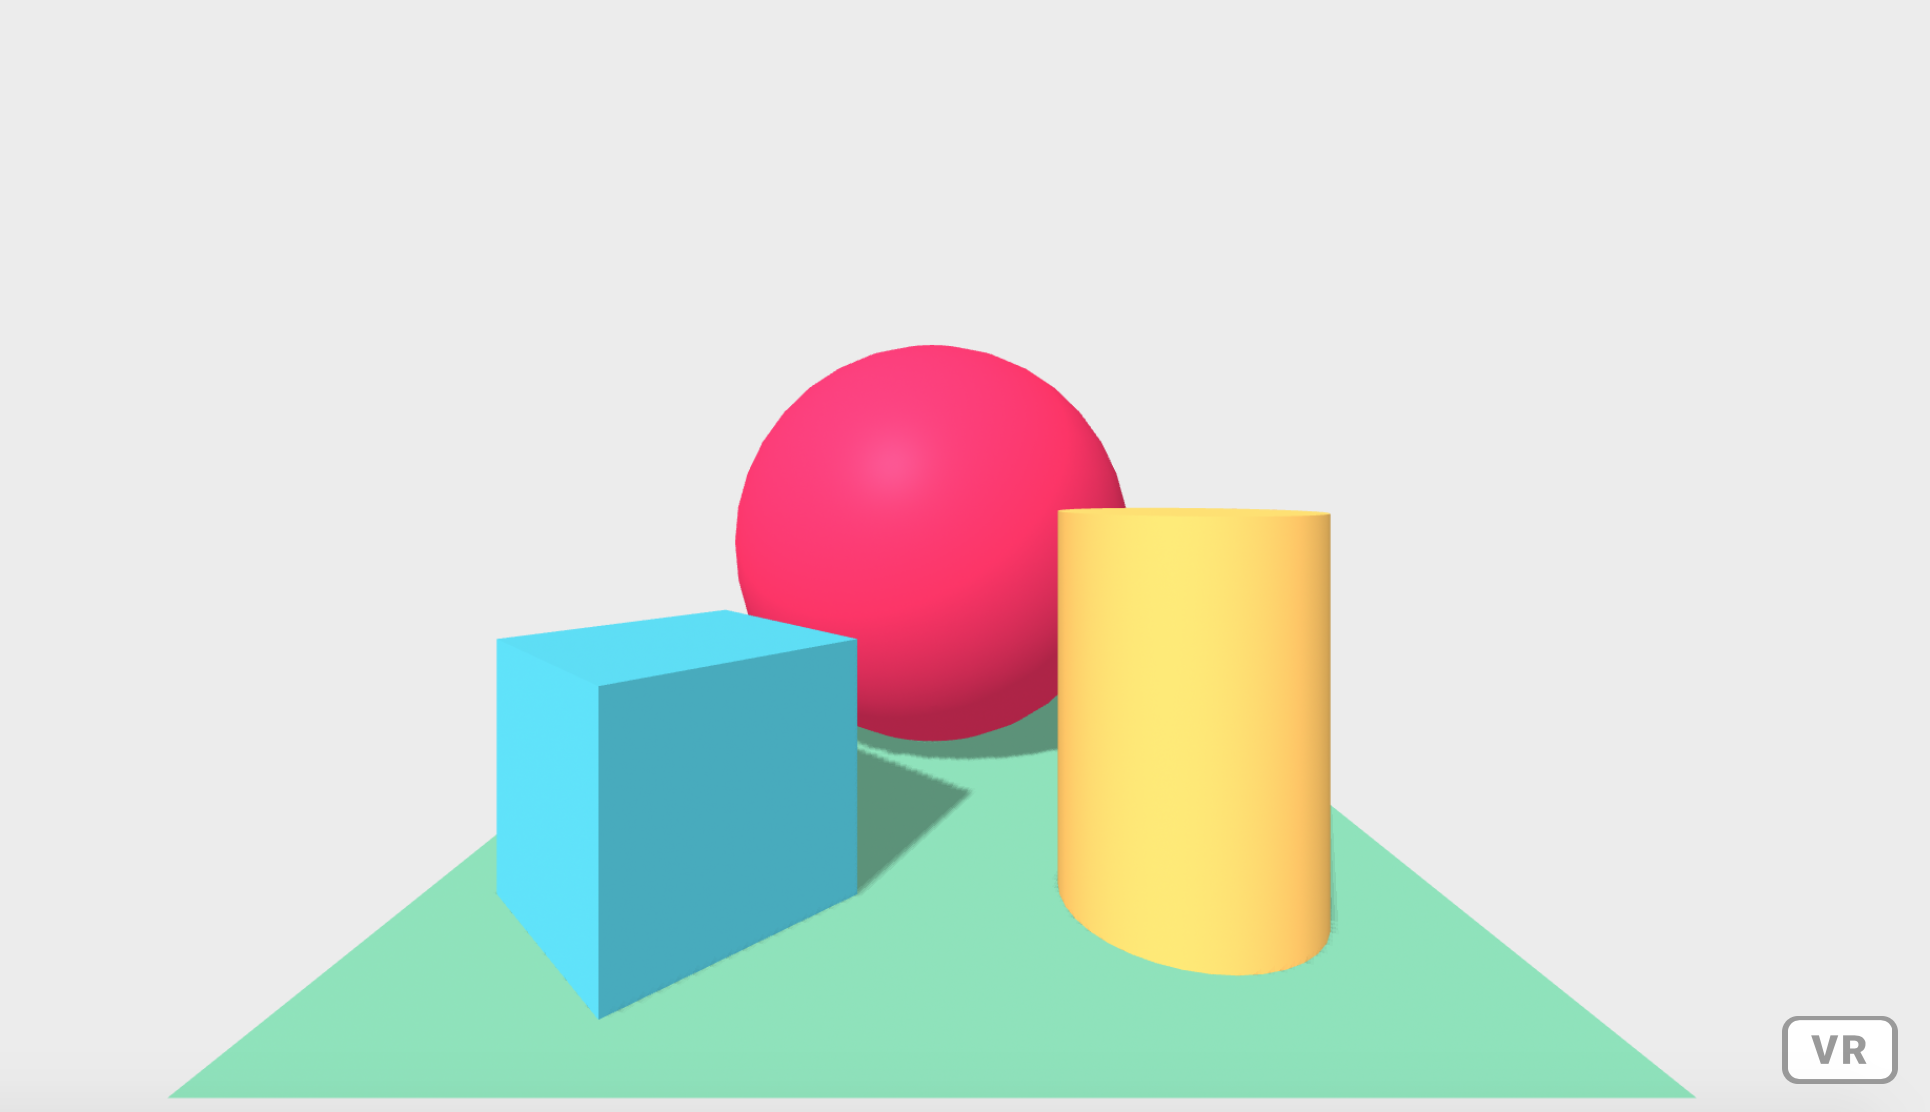
\includegraphics[width=12cm, keepaspectratio]{img/development/aframe.png}
  \caption{Ejemplo de A-Frame}
  \label{fig:aframeexample}
\end{figure}

\subsection{THREE.JS}
Es una biblioteca escrita en Javascript que permite la creación y visualización de objetos 3D en entornos web\cite{dirksen:_threejs}. Es muy convenientes pues permite utilizarse en conjunto con Canvas (HTML5) SVG y WebGL. Por lo que podemos decir que es compatible con cualquier navegador que soporte WebGL.

Además, permite importar modelos 3D, en formato JSON,  creados en Maya, Blender o Max3D.

\begin{figure}[H]
  \centering
  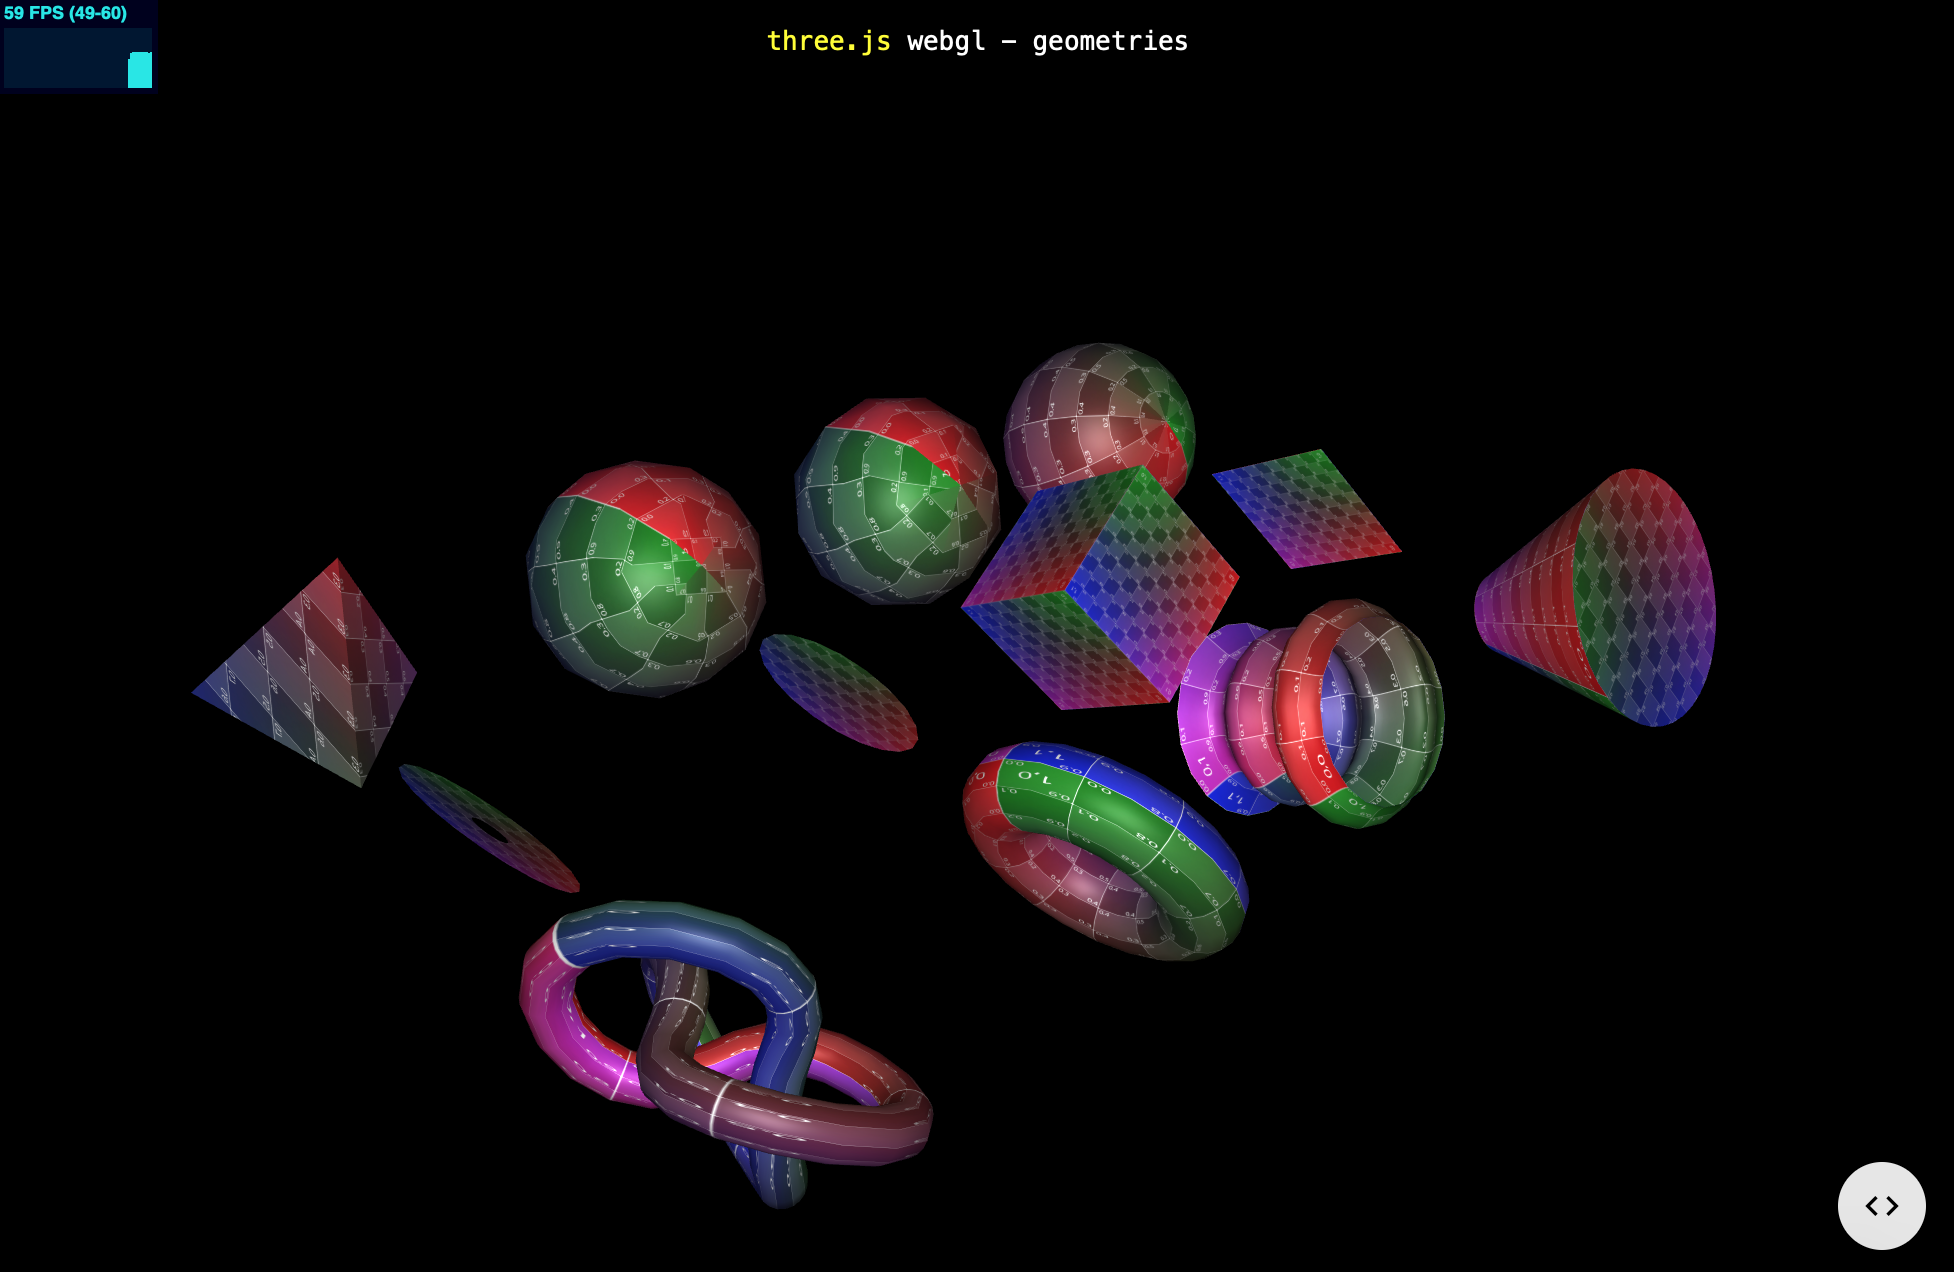
\includegraphics[width=12cm, keepaspectratio]{img/development/threejs.png}
  \caption{Ejemplos de figuras en three.js}
  \label{fig:threeexample}
\end{figure}

\subsection{En este proyecto}
A-Frame supone una parte importante de este proyecto, pues el objetivo de este proyecto es crear un plugin que permita dar una experiencia VR a la hora de representar la visualización de los datos mostrados en Kibana. 


%%%%%%%%%%%%%%%%%%%
% ELASTICSEARCH
%%%%%%%%%%%%%%%%%%%

\section{ELK}
\label{sec:elastic}
\subsection{Definición}
Es un conjunto de herramientas de gran potencial que ayuda con la administración de registros, permitiendo monitorizar, consolidar y analizar logs (no siempre son logs) generados en distintos servidores.
 
Estas herramientas son: Elasticsearch, Logstash y Kibana. Las tres se complementan entre sí pero, se pueden utilizar de forma independiente.

\begin{figure}[H]
  \centering
  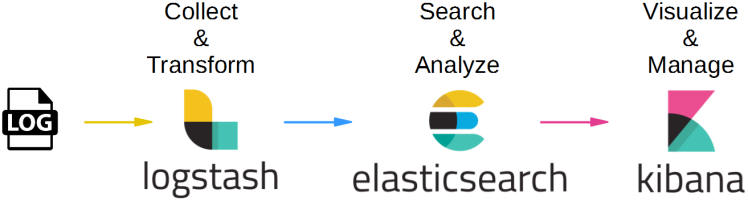
\includegraphics[width=12cm, keepaspectratio]{img/development/elk.png}
  \caption{Flujo de trabajo de ELK}
  \label{fig:diagramaelk}
\end{figure}

A continuación definiremos estas herramientas y su papel en este proyecto, dejando a Kibana para otro apartado debido a su importancia dentro del mismo.

\subsection{Elasticsearch}
Se trata de un motor de busqueda y analisis fácilmente escalable. Permite almacenar, buscar y analizar grandes volúmenes de datos casi en tiempo real. Se puede acceder de forma sencilla gracias a su elaborada API\cite{srivastava:_elasticguide}.

Está escrito en Java, de código abierto y generalmente utilizado con fines empresariales o de investigación.
\subsubsection{Características}
\begin{itemize}
\item \underline{Documentos}: está orientado a documentos que se insertan en formato JSON, son esquemas sin indexar. Lo que permite una búsqueda mucho mas rápida.
\item \underline{API}: cuenta con una potente API muy fácil de usar. Ésta permite hacer peticiones de tipo HTTP.
\item \underline{Rapidez}: Gracias a su distribución de escalado dinámico; Elasticsearch encuentra rápidamente cualquier consulta que se le haga, incluso cuando tenemos grandes cantidades de datos. Ya sean búsquedas simples, como complejas.
\item \underline{Gran componente}: Elasticsearch junto con Kibana y Logstash forman un conjunto de herramientas perfecta para la recopilación, análisis y visualización de datos.
\item \underline{En tiempo real}: Las actualizaciones de los índices de Elasticsearch se realizan de manera tan rápida que práticamente se puede consultar en tiempo real.
\end{itemize}
\subsubsection{En este proyecto}
Para este proyecto, no es una parte importante; pues solo la utilizaremos para indexar los datos de prueba que vamos a visualizar posteriormente en Kibana.


\subsection{Logstash}
Es la herramienta encargada de recolectar los logs de una aplicación, parsearlos; traducirlos y pasarlos a formato JSON para luego poder almacenarla en Elasticsearch. 

\subsubsection{En este proyecto}
Esta parte no la utilizaremos en este proyecto en ningún momento.

%%%%%%%%%%%%%%%%%%%%
% Kibana
%%%%%%%%%%%%%%%%%%%%

\section{Kibana}
\label{sec:Kibana}
\subsection{Definición}
Es una plataforma que permite visualizar los datos almacenados en Elasticsearch, para su posterior monitorización y análisis de estos desde el propio navegador web\cite{srivastaba:_kibanaguide}.

Al tratarse de código abierto, la propia empresa invita a que desarrolladores puedan contribuir con su mejoría o a la creación, como en nuestro caso, de plugins para personalizarlos al gusto del usuario. 
\subsubsection{Características}
\begin{itemize}
\item \underline{Visualizaciones}: podemos encontrar representaciones con histogramas, gráficas de tiempo, roscos o tablas que nos permite visualizar e interactuar con los datos almacenados en Elasticsearch.
\item \underline{Datos en tiempo real}: la buena conectividad entre ellos, permite visualizar y buscar la información unos pocos segundos después de ser introducida en Elasticsearch.
\item \underline{Dashboards}: que recogen las visualizaciones en paneles para poder tener una vista global y así poder entender mejor grandes cantidades de datos.
\item \underline{Geolocalización}: en caso de tener datos de ubicaciones; ésta te muestras las distintas coordenadas en mapas.
\item \underline{Extras}: también incluyen extras como timeseries, graphs o machine learning.
\end{itemize}

\begin{figure}[H]
  \centering
  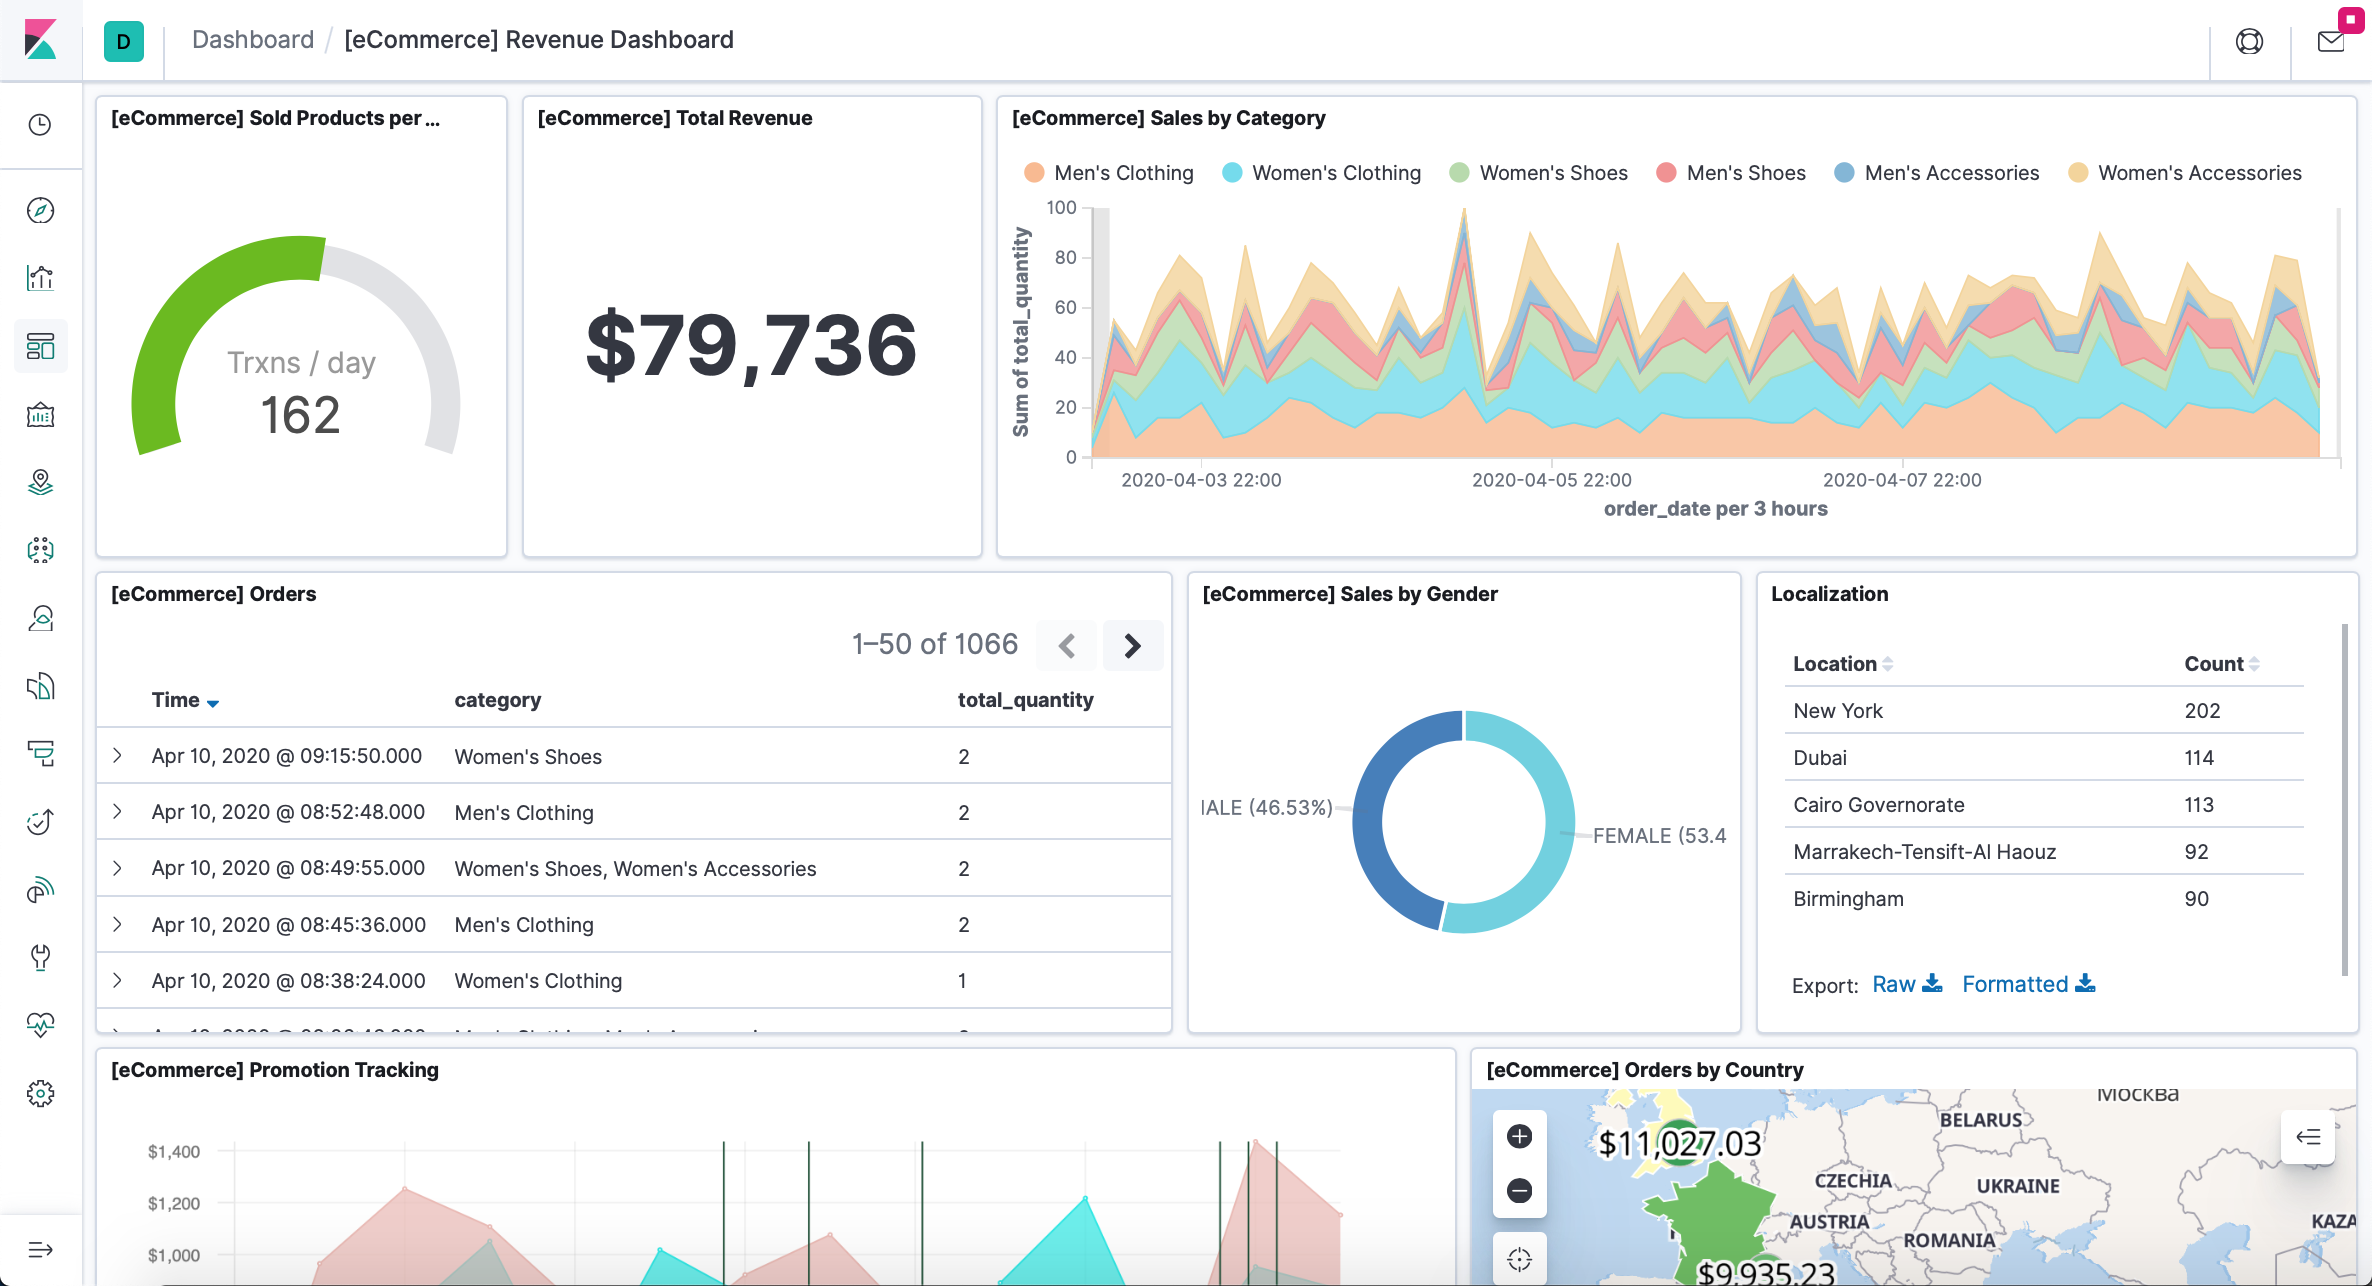
\includegraphics[width=12cm, keepaspectratio]{img/development/kibana-dashboard.png}
  \caption{Ejemplo de Dashboard en Kibana}
  \label{fig:kibanaexample}
\end{figure}


\subsection{En este proyecto}
Esta es la base de dicho proyecto, pues lo que queremos es crear un plugin que permita modificar los distintos tipos de visualizaciones en formato 3D, aportando esa experiencia en VR que tanto queremos conseguir.


%%%%%%%%%%%%%%%%%%%
% NODEJS
%%%%%%%%%%%%%%%%%%%

\section{NodeJS y NPM}
\label{sec:nodejs}
\subsection{Definición}
Node.js \cite{syed:_nodejs} es un entorno de ejecución basado en Javascript que aprovecha su capacidad para gestionar llamadas asíncronas y eventos. Es de código abierto y multiplataforma. Se utiliza principalmente en la capa de servidor.


NPM, también llamado \textit{Node Package Manager}\footnote{\url{https://docs.npmjs.com}}, es un gestor de paquetes para node.js. Nos permite instalar y desinstalar dependencias y aplicaciones que se encuentran en el repositorio desde la línea de comandos. Está escrito en javascript y viene incluído por defecto en todas las versiones de node.js desde la 0.6.3.

\subsection{En este proyecto}

NPM lo utilizamos para instalar todas las dependencias que necesitamos para añadirlas en nuestro código. Esto se hace desde el archivo \textit{package.json} y se instalan usando el comando \textit{``npm install"}, guardandose dentro el directorio \textit{node\_module}.

En cuanto a NodeJS, se utiliza para lanzar el cliente de Kibana y el servidor de Elasticsearch que viene dentro del entorno de desarrollo.

%%%%%%%%%%%%%%%
%BABIAXR
%%%%%%%%%%%%%%%

\section{BabiaXR}
\label{sec:babiaxr}
\subsection{Definición}

Es un biblioteca de componentes para crear visualizaciones gráficas de datos desarrollada con A-Frame\footnote{\url{https://github.com/babiaxr/aframe-babia-components}}. 

Esta colección de componentes permite visualizar datos tanto si esos datos son introducidos de forma manual o a traves de una petición. El formato con el que trabajan estos datos es JSON.

Existen varios tipos de componentes:
\begin{itemize}
    \item \underline{geopiechart}: genera una gráfica tipo pie.
    \item \underline{geosimplebarchart}: genera una gráfica de barras.
    \item \underline{geo3dbarchart}: genera una gráfica de barras, pero usando tres ejes en vez de dos.
    \item \underline{geobublechart}: genera una grafica de tipo bubble.
\end{itemize}

\begin{figure}[H]
  \centering
  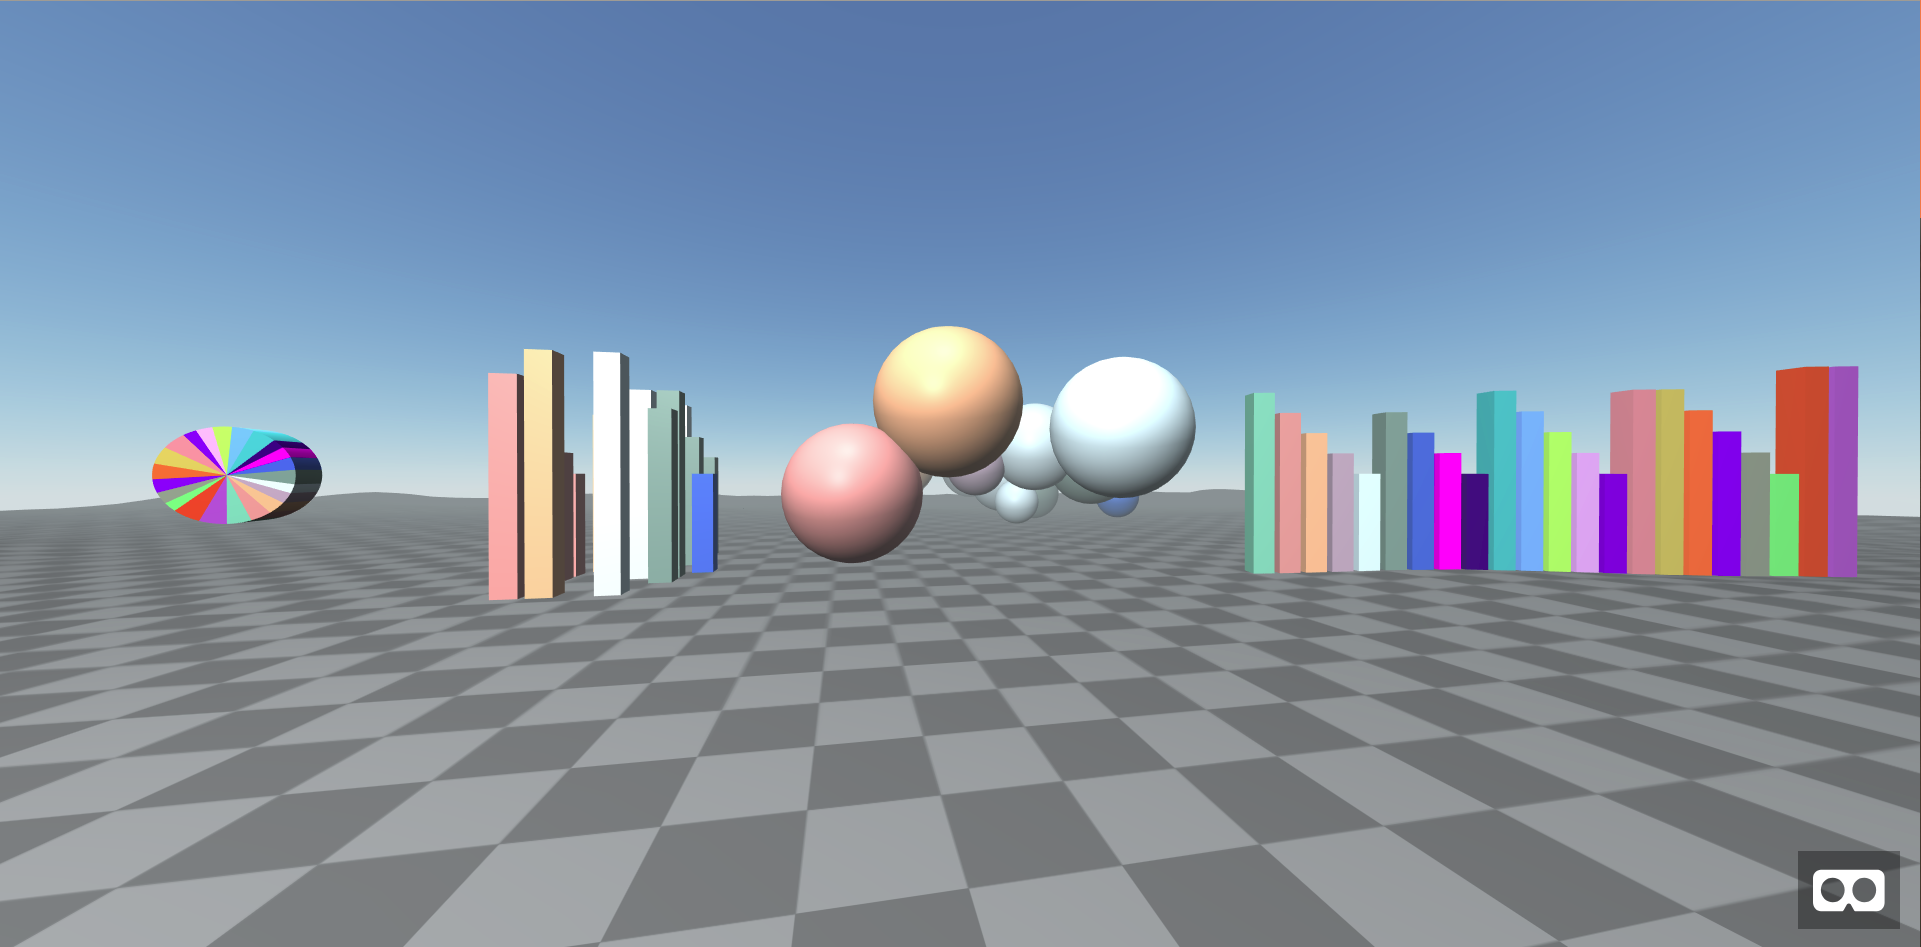
\includegraphics[width=12cm, keepaspectratio]{img/development/babiaxrcomponents.png}
  \caption{Tipos de Componentes de BabiaXR}
  \label{fig:babiacomponents}
\end{figure}

\subsection{En este proyecto}

Es otra de la partes importantes de este desarrollo, pues es la biblioteca que utilizamos para crear las visualizaciones de nuestro plugin.


%%%%%%%%%%%%%%%%%%%%%%%%%%%%%%%%%%%%%%%%%%%%%%%%%%%%%%%%%%%%%%%%
% DESARROLLO %
%%%%%%%%%%%%%%%%%%%%%%%%%%%%%%%%%%%%%%%%%%%%%%%%%%%%%%%%%%%%%%%%

\cleardoublepage
\chapter{Desarrollo}
\label{sec:desarrollo} 

En este capítulo se describe cómo se ha organizado este proyecto y qué se ha desarrollado en cada una de sus iteraciones. En ellas se mostrará también los trozos de código e imágenes resultantes.

%%%%%%%%%%%%%%%%%%%
% METODOLOGIA SCRUM
%%%%%%%%%%%%%%%%%%%

\section{Metodología SCRUM}
\label{sec:scrum}

 Para el desarrollo de este proyecto nos hemos organizado usando una versión inspirada en la metodología SCRUM\cite{sutherland:scrum}. La metodología SCRUM\footnote{\url{https://www.scrum.org/resources/blog/que-es-scrum}} es un marco de trabajo que se utiliza dentro del desarrollo ágil de software. 

A diferencia de otros métodos donde el desarrollo va de manera secuencia o el cascada, SCRUM permite desarrollar en pequeñas fases que van incrementando hasta llegar al objetivo final. Esto permite analizar cada fase y reorganizar, en caso de que sea necesario, durante el proceso. 

\begin{figure}[H]
  \centering
  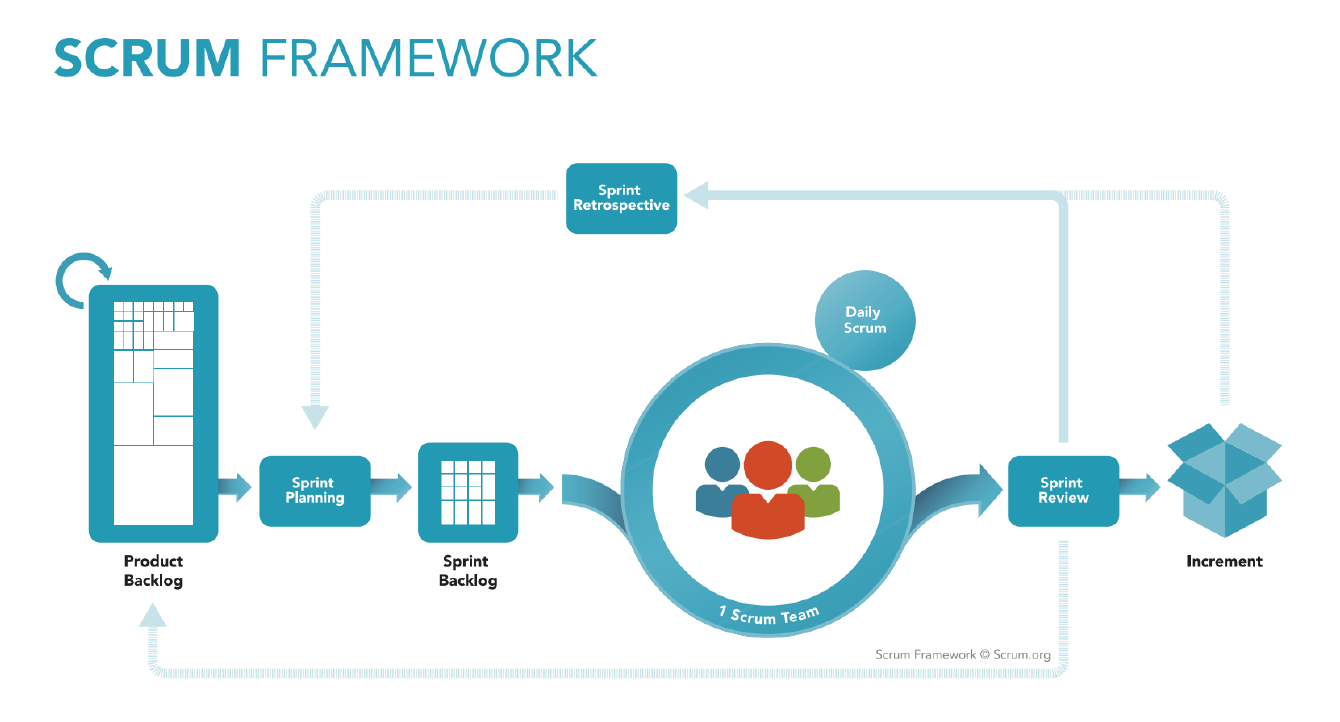
\includegraphics[width=12cm, keepaspectratio]{img/development/scrum.png}
  \caption{Diagrama de la Metodología SCRUM}
  \label{fig:scrum}
\end{figure}

Para gestionar este control, se definen diferentes roles:

\begin{itemize}
    \item \underline{Product owner}: es el responsable de optimizar y maximizar el valor del producto final. Todo esto lo gestiona a través del product backlog y hace de interlocutor con los stakeholders.
    \item \underline{SCRUM master}: es el responsable de que se siga la metodología según sus reglas y ayuda a eliminar los impedimentos que puedan afectar a la entrega final del producto.
    \item \underline{Development Team}: es un equipo pequeño que se encarga de desarrollar el producto, para ello deben auto-organizarse para conseguir entregar el incremento de software que se les pide al final de esa fase de desarrollo o sprint.
\end{itemize}


En este proyecto solo utilizaremos los conceptos para definir los distintos roles. Este equipo se compone de dos personas: el tutor y el autor del proyecto. Es por eso que distribuimos los roles de la siguiente manera:

\begin{itemize}
    \item \textit{Product owner} y \textit{SCRUM master} serán representado por el tutor del proyecto.
    \item \textit{Development Team} será representado por el autor del proyecto.
\end{itemize}

Estas pequeñas fases incrementales reciben el nombre de \textit{sprint} o \textit{iteración}. Es un bloque de tiempo, no superior a un mes, en el cual se desarrolla el incremento del producto. Durante el sprint se dan varios eventos:

\begin{itemize}
    \item \underline{Sprint Planning}: se realiza siempre al principio del sprint y responde a las siguientes preguntas: ¿qué se puede entregarse en el incremento?; y ¿cómo se va a hacer para llegar a dicho incremento?
    \item \underline{Daily Sprint}: reunión diaria donde se pone al día como va avanzando el sprint y se planea el trabajo de dicho día.
    \item \underline{Sprint Review}: se realiza al final de cada sprint donde se revisa que objetivos del product backlog se han cumplido o si es necesario modificar algún elemento.
    \item \underline{Sprint Retrospective}: se realiza de cara al siguiente sprint donde el equipo de desarrollo se analiza con la intención de mejorar.
\end{itemize}

En este modelo prescindimos del Daily Sprint. Los otros tres los unificamos en una misma sesión, donde al finalizar un sprint, analizamos el producto final de dicho sprint y planificamos el siguiente. 


Partiendo de esto, describiremos brevemente cada uno de los sprints o iteraciones por las que ha pasado este proyecto:

\begin{itemize}
    \item \underline{Iteración 0}: Investigación y estudio preliminar de las herramientas con las que vamos a trabajar.
    \item \underline{Iteración 1}: Creación de los primeros plugins sin usar datos, implementación de A-Frame y creación de un componente A-Frame.
    \item \underline{Iteración 2}: Modificación del plugin anterior para crear visualizaciones a partir de datos de Elasticsearch.
    \item \underline{Iteración 3}: Integración de un componente de la biblioteca BabiaXR dentro de Kibana.
    \item \underline{Iteración 4}: Añadir nuevas visualizaciónes con el resto de componentes de BabiaXR.
\end{itemize}


%%%%%%%%%%%
% SPRINT 0
%%%%%%%%%%%

\section{Sprint 0: Investigación y Estudio Priliminar }
\label{sec:sprint0}

Antes de comenzar con el desarrollo, debemos estudiar un poco el funcionamiento de las herramientas con las que vamos a trabajar. Por eso, empezaremos con este sprint, que llamaremos sprint 0 porque uno será un sprint en sí. 

Primero será establecer las herramientas que necesitaremos conocer para llevar a cabo el desarrollo. Como nuestro objetivo es crear un plugin para visualizar gráfica en VR para Kibana, lo ideal sería que conociéramos un poco el funcionamiento de ésta. 

Luego crearemos un entorno de desarrollo para Kibana y documentarse cómo se crean plugins para Kibana.

Por último, exploraremos un poco con la biblioteca BabiaXR para conocer su funcionamiento.


%TESTEANDO CLIENTE Kibana
\subsection{Explorando el Cliente de Kibana}

Como se ha mencionado antes, lo primero que haremos será explorar el cliente de Kibana. Lo que haremos será instalar un Elasticsearch, que usaremos para que nos proporcione los datos; y un cliente de Kibana para que exploremos su funcionamiento.

Estas dos herramientas se pueden conseguir de forma gratuita en la web oficial de Elastic\footnote{\url{https://www.elastic.co/es/downloads}}. Descargamos las últimas versiones oficiales (\textit{versión 7.6}) y las instalamos en el propio equipo. Un dato a tener en cuenta es que ambos deben ser de la misma versión, sino no funcionará (o no funcionará correctamente). Para una primera vez, lo mejor es no tocar la configuración de ninguno de los dos programas.

Anteriormente se mencionó que Kibana era una manera de monitorizar los datos recopilados en Elasticsearch, pero aunque no tengamos ninguna base de datos en Elasticsearch, Kibana nos permitirá descargar unas bases de datos de prueba para que podamos utilizarlo en esta primera exploración. Para esta ocasión utilizaremos la base de datos de eCommerce.

Lo primero que nos encontramos es la pestaña \textit{Discover} que nos muestra una lista de todos los items que hay en la base de datos (en este caso, las ventas que se han realizado). A la izquierda, tenemos un editor que nos permite filtrar los campos que queremos que aparezca en el listado. Además, en la parte de arriba, justo encima de la tabla de datos, hay una gráfica que nos muestra una visualización gráfica de los datos que hemos filtrado, para esta ocasión el número de ventas que se realizan a lo largo del día.

\begin{figure}[H]
  \centering
  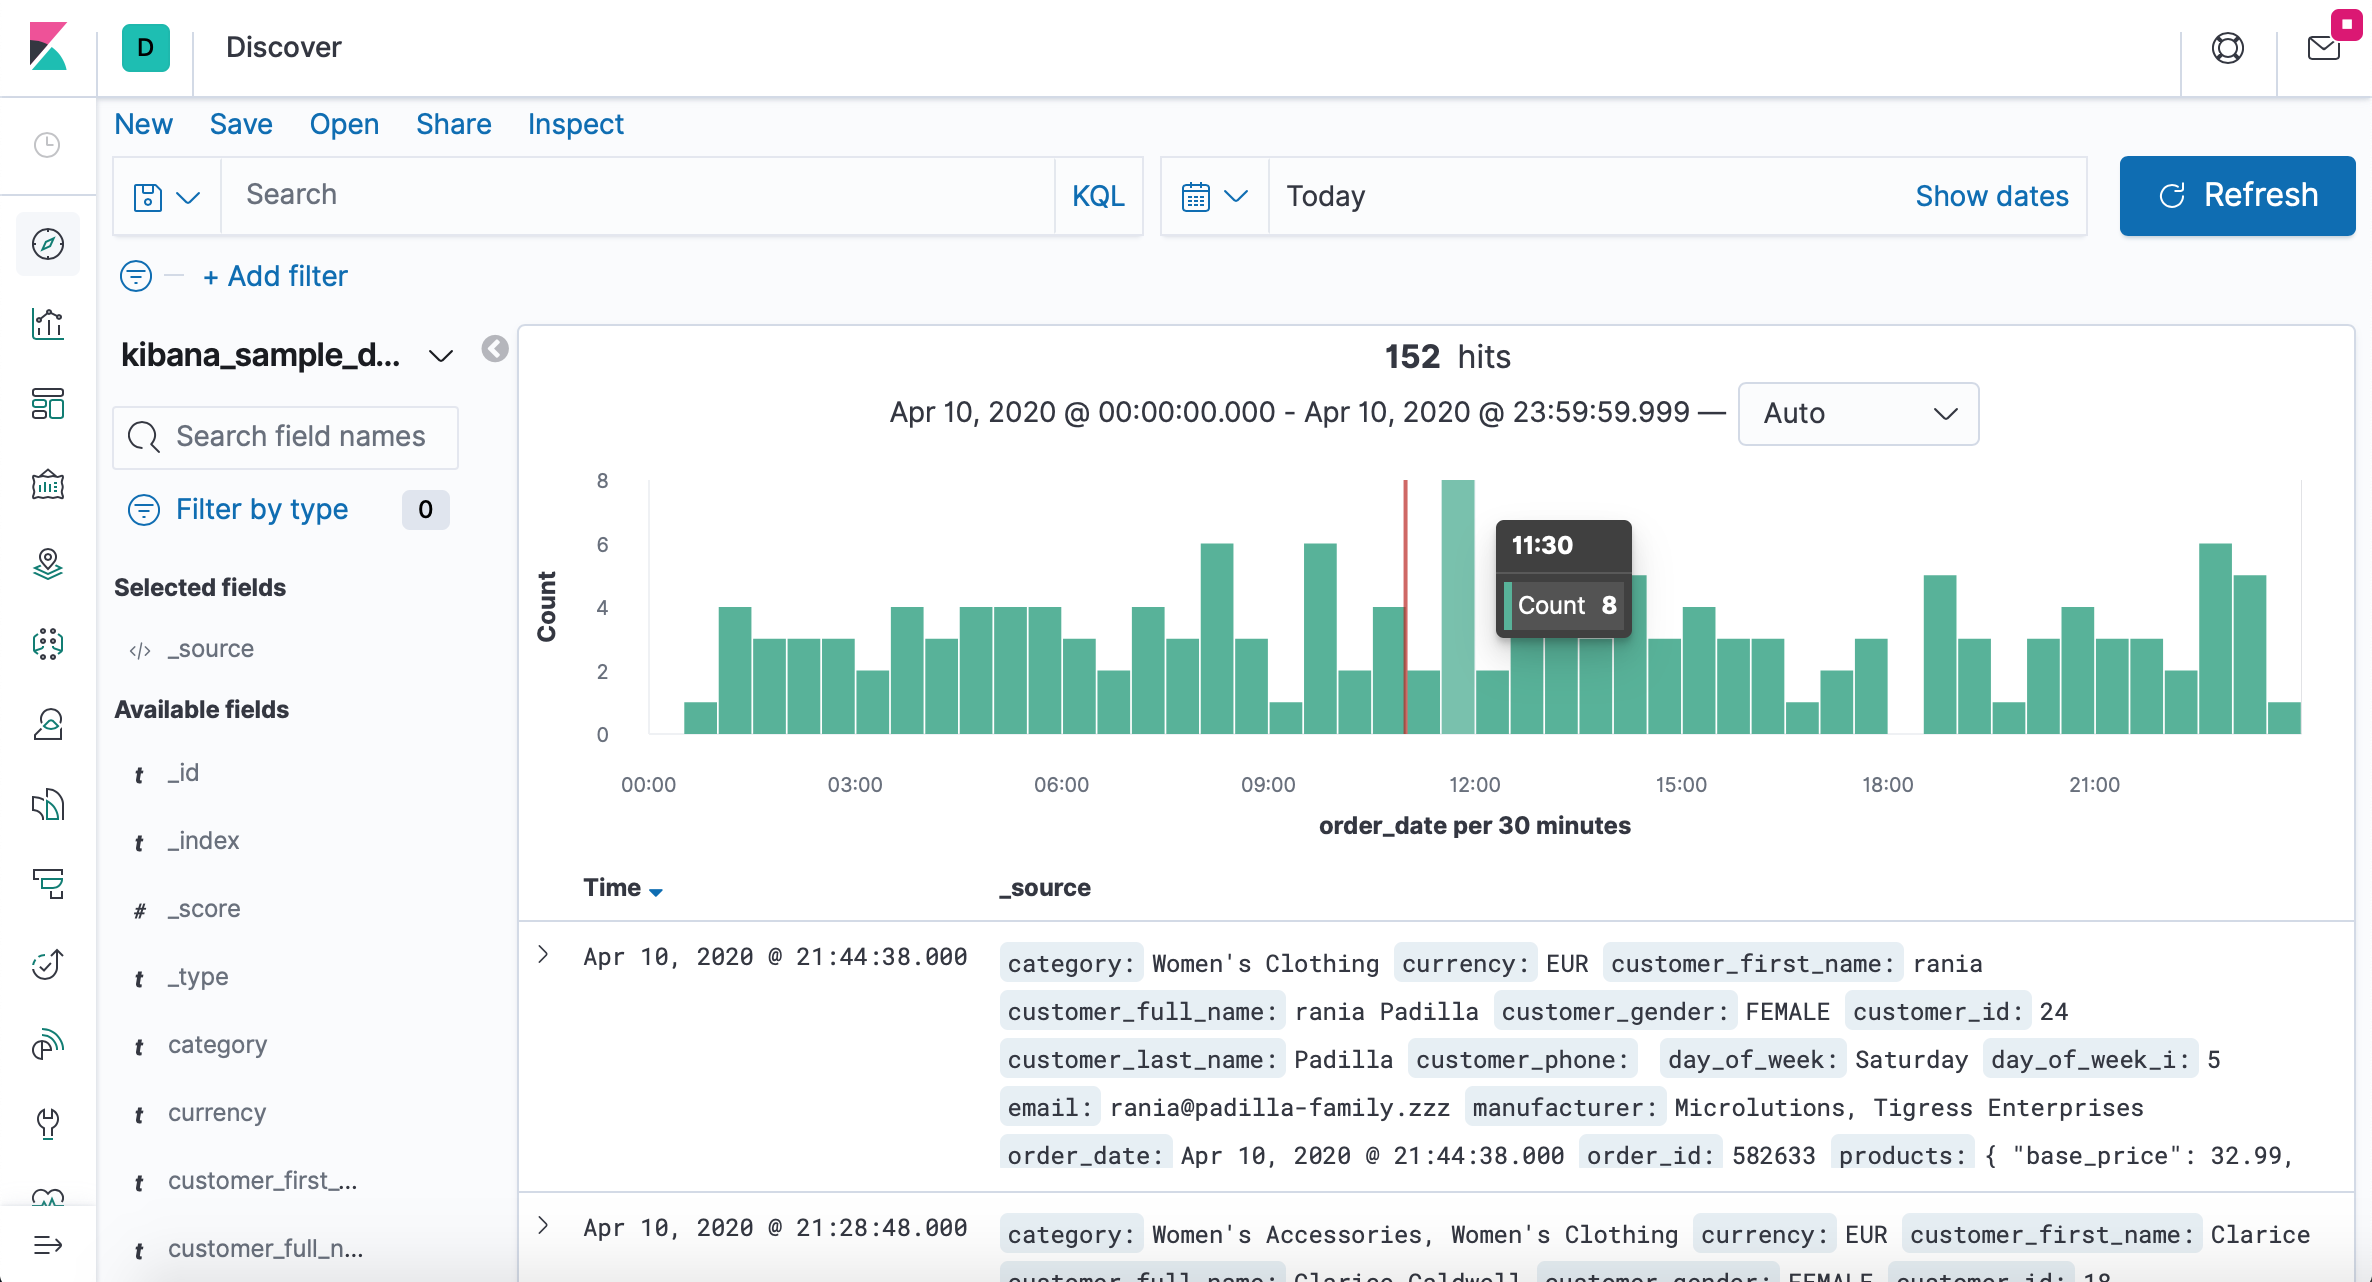
\includegraphics[width=12cm, keepaspectratio]{img/development/Discover-kibana.png}
  \caption{Pestaña Discover del cliente de Kibana}
  \label{fig:Kibanadiscover}
\end{figure}

Una vez que ya hemos comprendido, viéndolo en la pestaña de \textit{Discover}, con que clase de datos trabajamos; pasaremos a ver cómo se crean las visualizaciones. Para ello, iremos a la pestaña \textit{Visualization} y lo primero con lo que nos encontramos es con que, al habernos descargado datos de prueba, ya vienen unas predeterminadas. Antes de ponernos a probar a crear una, lo mejor será coger una de estas predeterminada para entender su funcionamiento.

Esta visualización nos muestra una gráfica tipo Pie que viene configurada para que nos muestre el número de ventas en base al género del cliente, ya sea hombre (MALE) o mujer (FEMALE). A mano izquierda vemos que existe también un editor que nos permite configurar la gráfica. Existen dos pestañas dentro de la misma:

\begin{itemize}
    \item \underline{Data}: donde configuraremos qué datos queremos que nos muestre, separados entre metrics y buckets (que explicamos más adelante).
    \item \underline{Options}: como su propio nombre indica, configuraciones opcionales. Por ejemplo, en este caso te permite indicarle donde se desea colocar la leyenda, o si queremos que la gráfica sea rellena o no.
\end{itemize}

\begin{figure}[H]
  \centering
  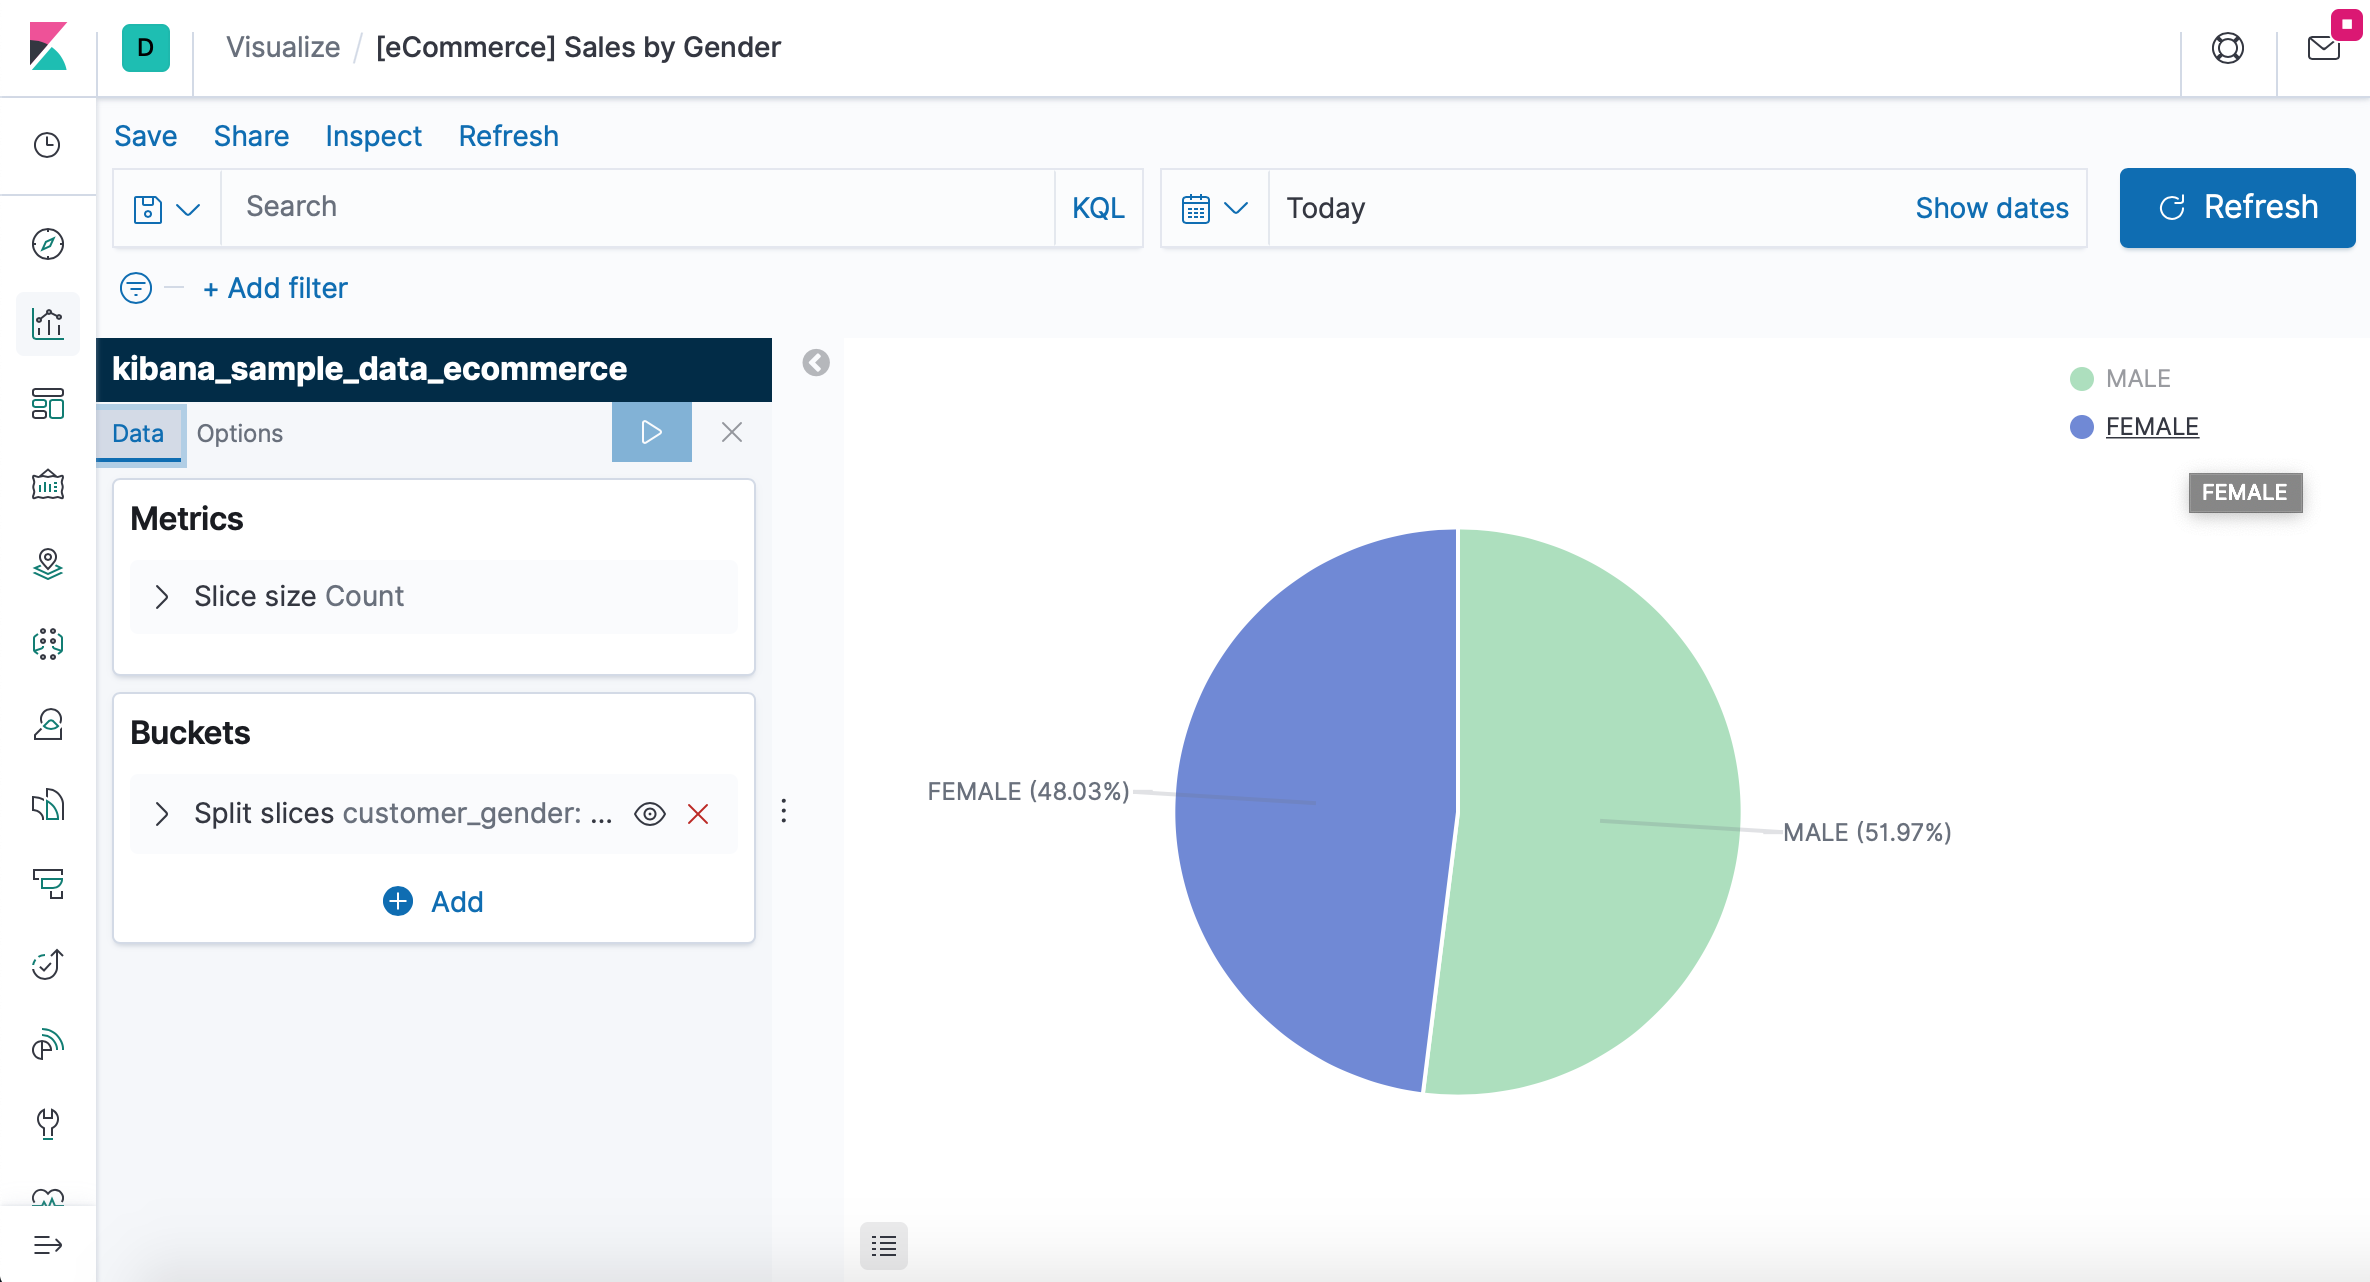
\includegraphics[width=12cm, keepaspectratio]{img/development/Kibana-visualization-pie.png}
  \caption{Visualizacion Pie en el cliente de Kibana}
  \label{fig:Kibanapie}
\end{figure}

Ahora que ya entendemos un poco el funcionamiento de las visualizaciones, pasaremos a crear una propia; pero que sea diferente de la anterior. Por ejemplo, nos interesa ver desde qué países se han realizado las ventas. Elegimos \textit{Create Visualization} y seleccionamos, para este caso, la visualización tipo Table. 

Como no nos queremos complicar mucho, lo único que haremos será pedirle que nos muestre la cantidad de ventas que se han realizado en base a los países. Para ello, vamos en la pestaña \textit{Data} y en metrics le indicamos \textit{Count} que nos mostrará la cantidad de ventas. Y luego \textit{Buckets} que nos los clasifique por país. Para ello, se ha de seleccionar en \textit{Aggregations} la opción de \textit{Terms} y luego en \textit{Field} le indicamos que queremos que se clasifique por nombre de país \textit{geoip.region\_name}. Además, nos permite que lo podamos ordenar de mayor a menor o viceversa; o que solo nos muestre, por ejemplo, los 5 primeros. O incluso, darle una etiqueta a los datos que estamos mostrando.

\begin{figure}[H]
  \centering
  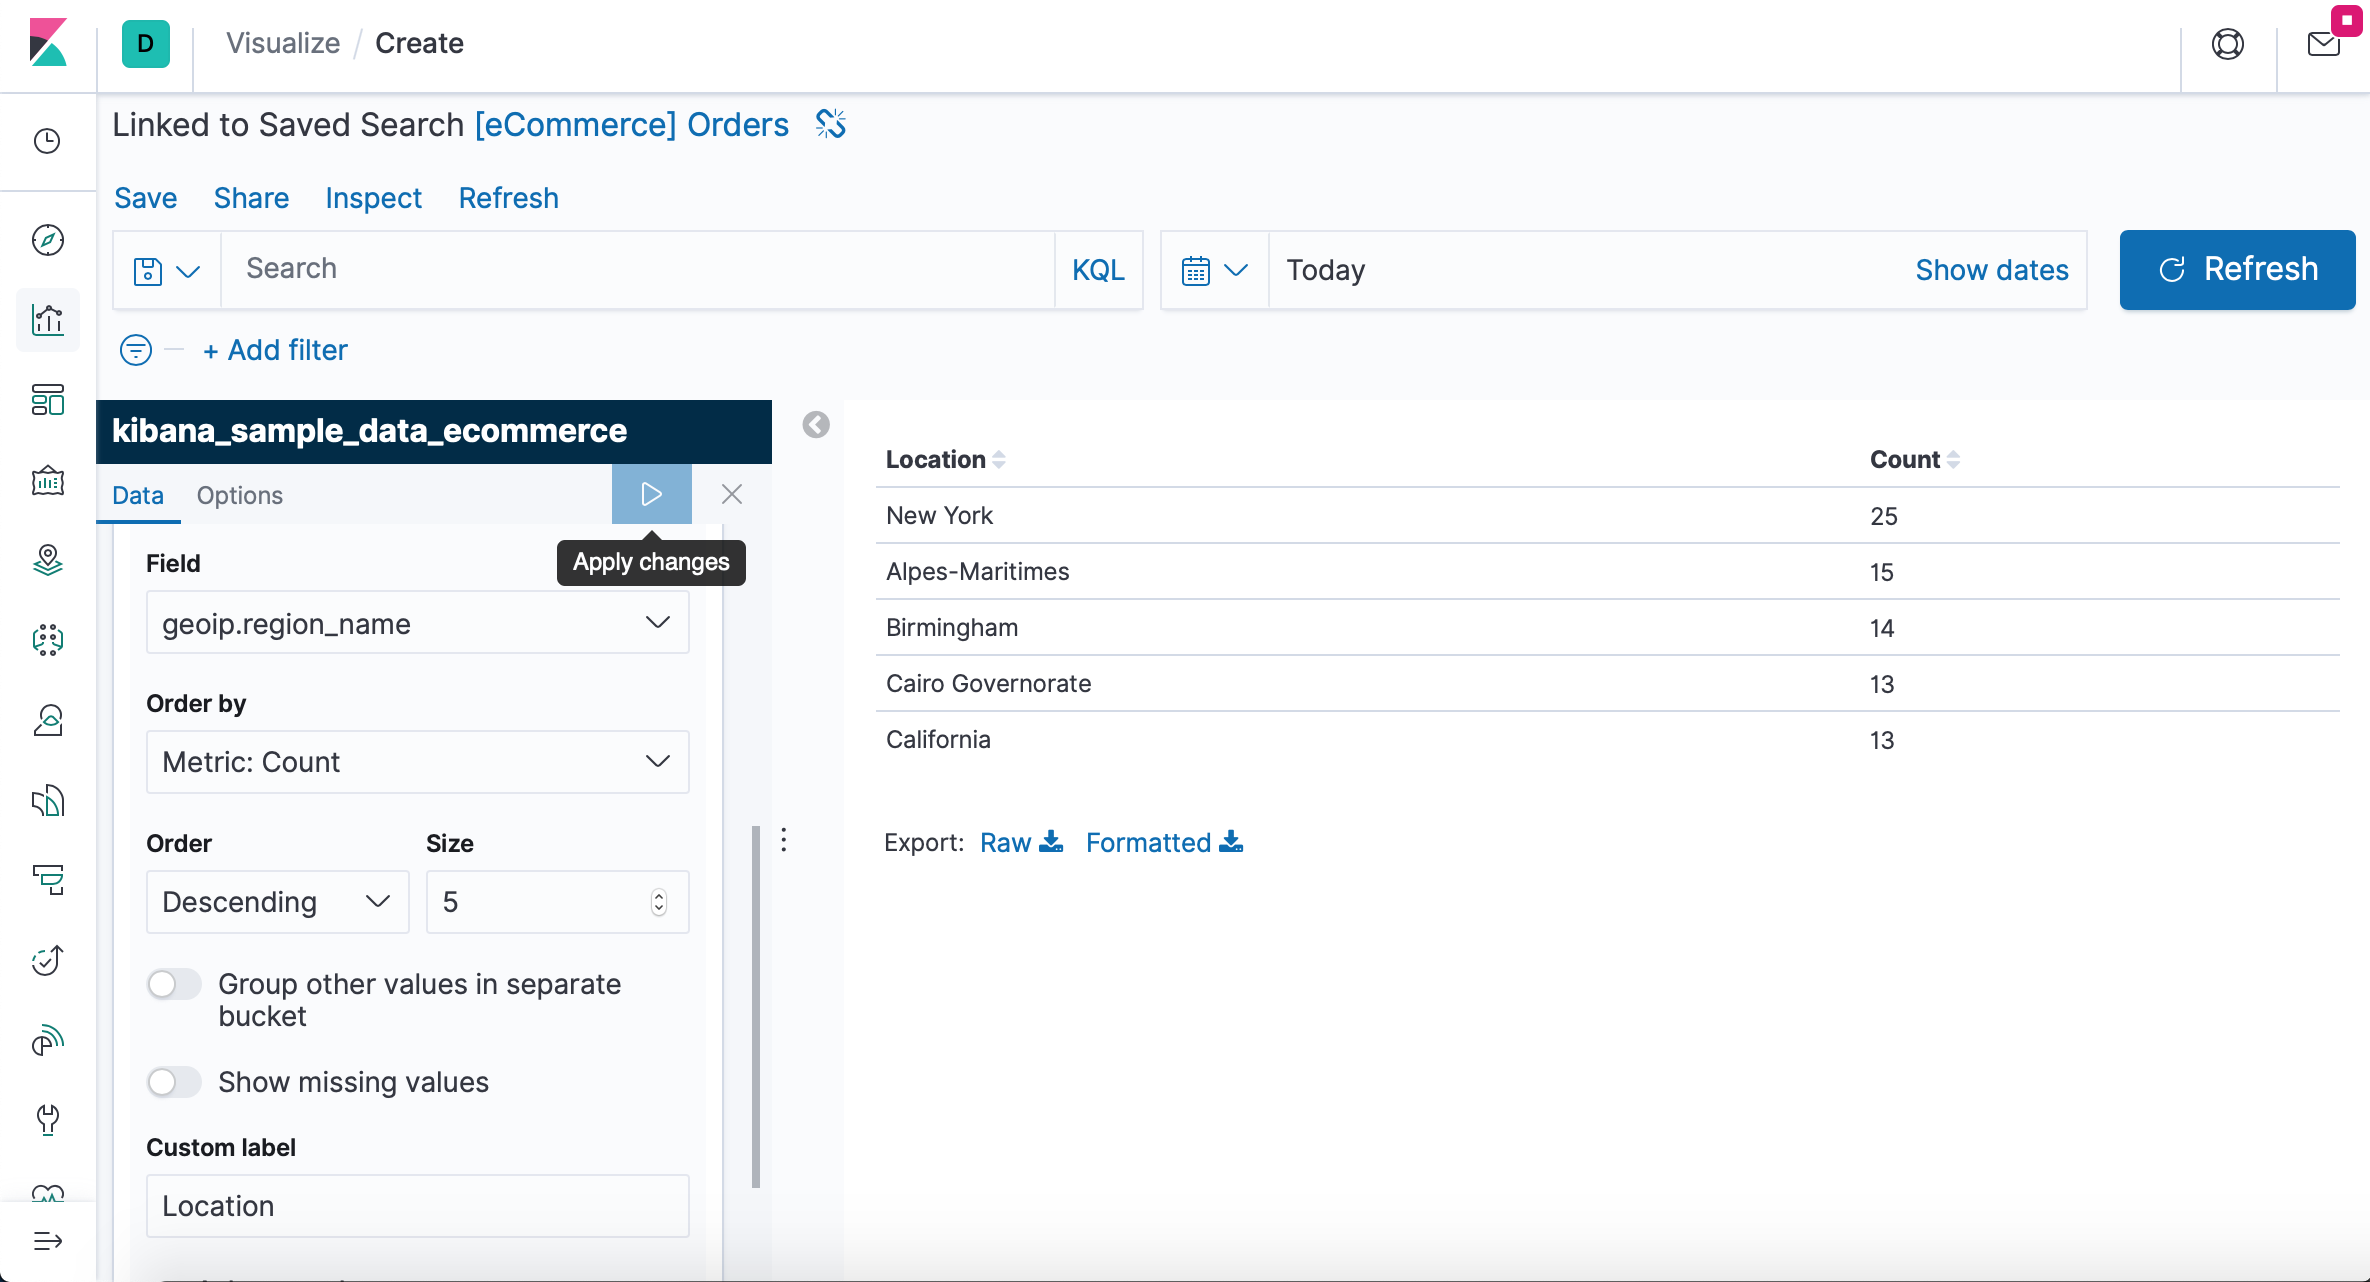
\includegraphics[width=12cm, keepaspectratio]{img/development/kibana-table-editor.png}
  \caption{Creación de Vizualización Table en el cliente de Kibana}
  \label{fig:Kibanatable}
\end{figure}

Una vez seleccionado cómo queremos nuestra visualización, solo tenemos que hacer click en \textit{Apply changes} y se actualizará al instante. Y una vez que tengamos la visualización que queremos, simplemente la guardamos dándole a \textit{Save}.

Después de haber probado alguna visualización y haber creado una propia, nos interesa conocer otra sección interesante y es la que encontramos en la pestaña \textit{Dashboard}. En esta, nos encontramos con que ya existe una predeterminada así que, aunque podemos crear una nueva, la editaremos.

Para entenderlo bien, la dashboard nos muestra en una misma página todas las visualizaciones que tenemos creadas y que queremos que sean mostradas. Lo que nos permite en edición es añadir o eliminar visualizaciones, colocarlas en un sitio u otro; o incluso darles el tamaño que nos interese.

\begin{figure}[H]
  \centering
  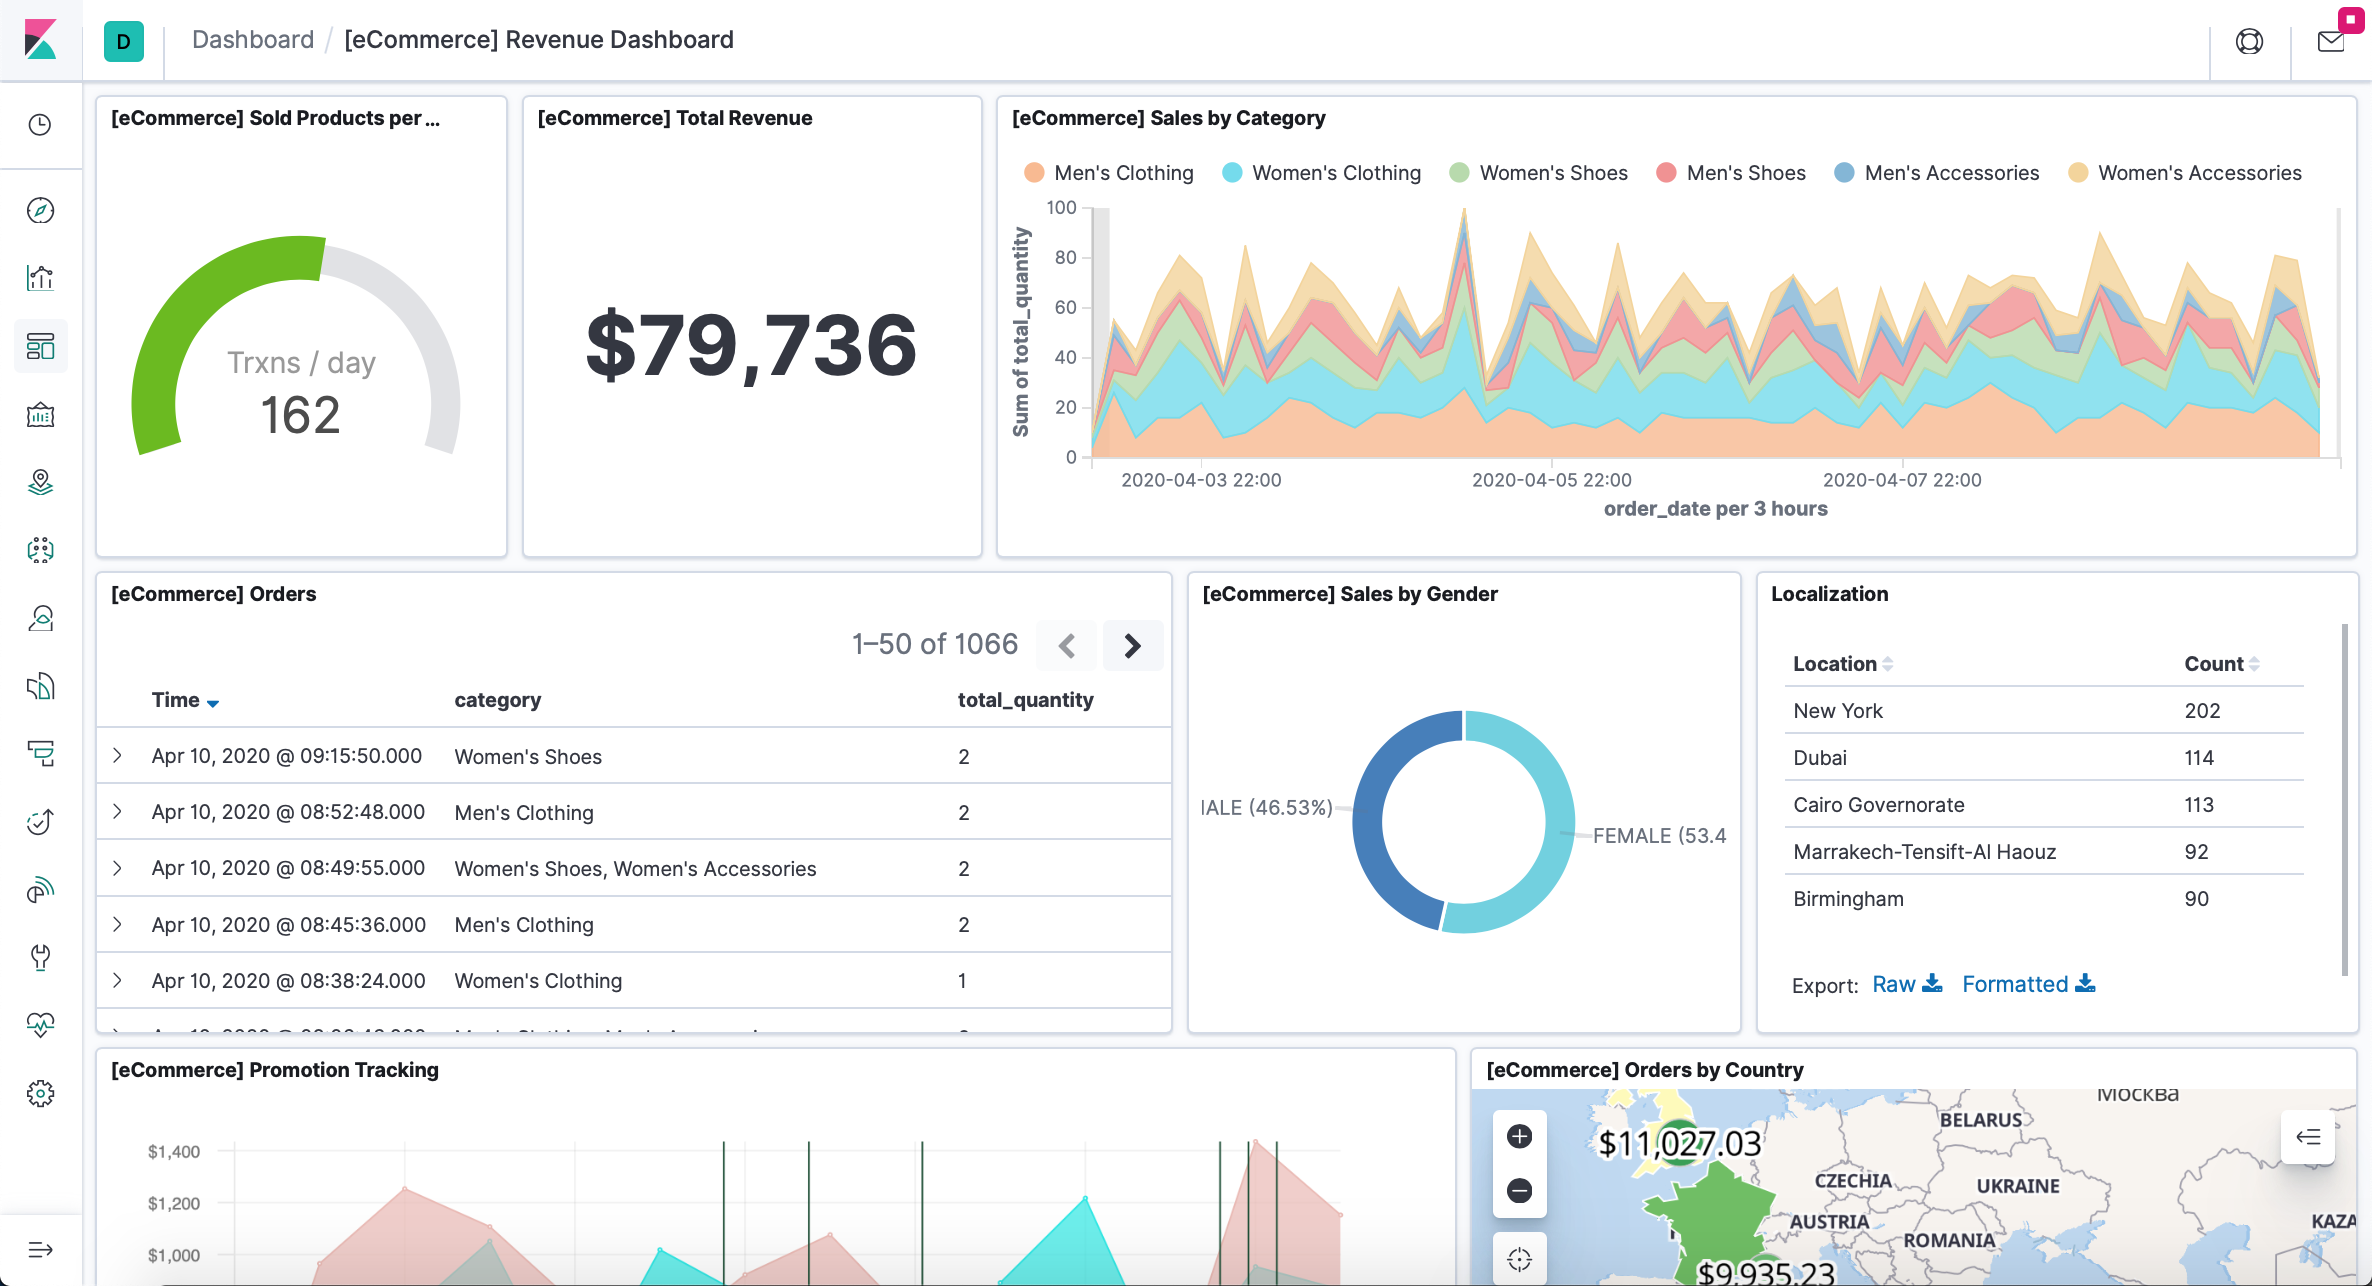
\includegraphics[width=12cm, keepaspectratio]{img/development/kibana-dashboard.png}
  \caption{Dashboard en el cliente de Kibana}
  \label{fig:Kibanadashboard}
\end{figure}


%CREANDO ENTORNO DE DESARROLLO
\subsection{Creando el Entorno de Desarrollo}
\label{sec:entorno}

Ahora que ya entendemos un poco el funcionamiento del cliente de Kibana, pasaremos a crearnos el entorno de desarrollo que utilizaremos para crear nuestro plugin. Este nos permitirá ver en tiempo real los cambios que realicemos.

Siguiendo las indicaciones que podemos encontrar en la sección correspondiente para contribuir en el proyecto \textit{CONTRIBUTING.md}\footnote{\url{https://github.com/elastic/kibana/blob/master/CONTRIBUTING.md}} dentro del repositorio de Kibana.

Una vez tengamos creado nuestro entorno de desarrollo, pasaremos a documentarnos cómo se crean plugins para Kibana. Para ello, Elastic nos proporciona artículos en su blog de como crear unos plugins básicos \footnote{\url{https://www.elastic.co/es/blog/developing-new-kibana-visualizations}}. Aunque está un poco obsoleta la documentación, únicamente nos quedaremos con la parte de cómo es la estructura de ficheros.

Por el momento no vamos a detallar el contenido de los ficheros (lo explicaremos más adelante en \ref{sec:holamundo}), simplemente nos enfocaremos en qué función tiene cada uno.

Lo primero que haremos será crear un directorio con en nombre de nuestro plugin dentro del directorio \textit{KIBANA\_HOME/plugins}. Y crearemos los siguientes ficheros:

\begin{itemize}
    \item \underline{package.json}: un simple fichero para npm donde le indicamos el nombre de nuestro plugin, version, autor, etc. Y sobretodo, las dependencias que necesitamos que nos instale para poder utilizarlas en nuestro proyecto.
    \item \underline{index.js}: este es el módulo principal. En él registramos nuestro plugin indicando el tipo de plugin (dentro de Kibana) que es, visualización en este caso; y hacemos referencia al fichero principal.
\end{itemize}

A esto le sigue crear un nuevo directorio con el nombre \textit{public/} que contendrá todos los ficheros de nuestro plugin (controllers, configurations, templates, etc). Antes hemos dicho que desde \textit{index.js} hacíamos referencia a el fichero principal de nuestro plugin, pues es aquí donde lo crearemos.

\begin{itemize}
    \item \underline{public/plugin-name.js}: para el caso de las visualizaciones es donde registramos las diferentes visualizaciones, puede ser una o varias, que vamos a añadir en Kibana a través de nuestro plugin.
\end{itemize}

Todos los ficheros anteriormente mencionados son los principales para el funcionamiento de esto; pero a mayores se le pueden añadir más ficheros. Algunos ejemplos opcionales:

\begin{itemize}
    \item \underline{public/plugin-name-controller.js}: como su propio nombre indica, sería el controlador de nuestro plugin. En el contiene toda la parte lógica de nuestra visualización.
    \item \underline{public/plugin-name.html}: template del plugin.
    \item \underline{public/plugin-name.less}: hoja de estilo del plugin.
    \item \underline{public/options-template.html}: template para la pestaña \textit{Options} del editor.
\end{itemize}

De forma más visual, podemos decir que la estructura de ficheros para que necesitamos para la creación de un plugin para Kibana es la siguiente:

\begin{lstlisting}[frame=single]
Kibana_HOME/plugins/
|___ plugin-name/
    |___ package.json
    |___ index.js
    |___ public/
        |___ plugin-name.js
        |___ plugin-name-controller.js
        |___ plugin-name.html
        |___ plugin-name.less
        |___ options-template.html
\end{lstlisting}


%TESTEANDO BIBLIOTECA PARA LAS VISUALIZACIONES
\subsection{Explorando la Biblioteca para las Visualizaciones}

Al igual que necesitamos conocer el funcionamiento de Kibana, también necesitamos tener unos conceptos básicos sobre los componente visuales que vamos a incorporar para nuestras visualizaciones para Kibana.

La opcion de usar BabiaXR ha sido muy acertada, ya que permite crear gráficas, a partir de datos proporcionados, dentro de un escenario WebXR. Así que antes de nada, analizaremos lo que nos ofrece y cómo se crean.

Dentro del repositorio de BabiaXR podemos ver los distintos tipos de componentes que tienen creados. Dichas componentes han sido creadas a partir del framework A-Frame (cápitulo \ref{sec:aframe}).

Lo primero que haremos será probar los diferentes componentes que tienen: \textit{geopiechart}, \textit{geosimplebarchart}, \textit{geo3dbarchart} y \textit{geobubblechart}. Todas ellas se pueden probar desde su web.

\begin{figure}[H]
  \centering
  \minipage{0.32\textwidth}
  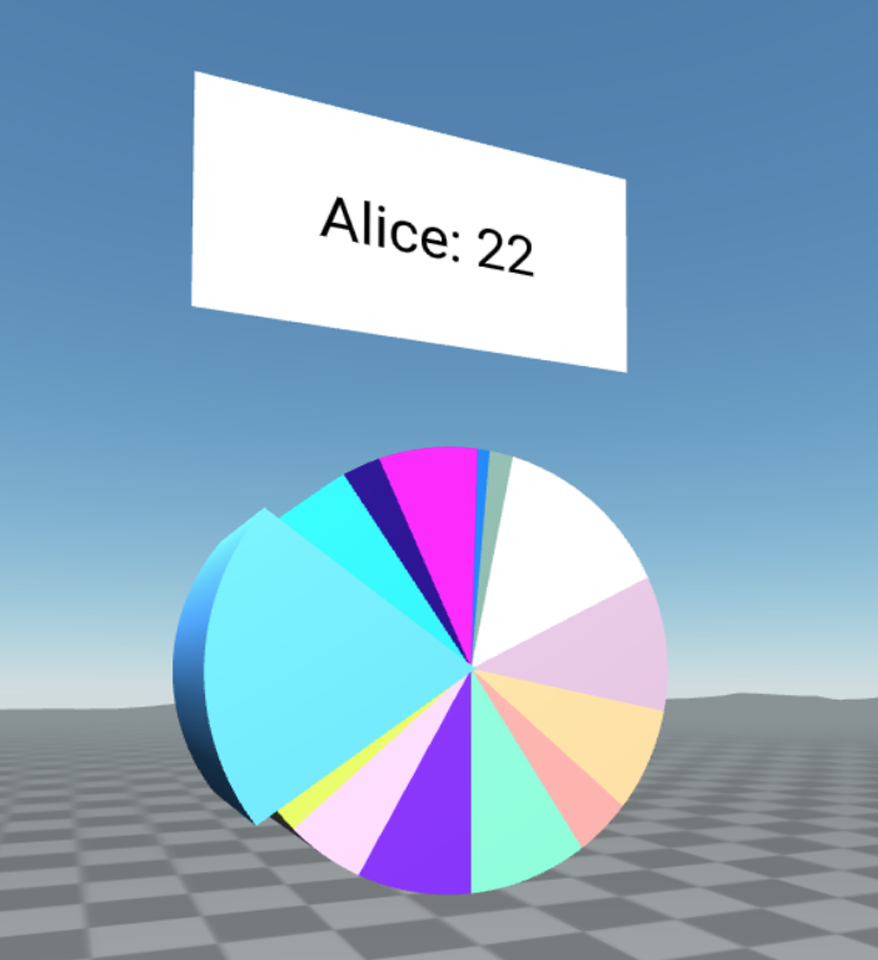
\includegraphics[width=5cm, keepaspectratio]{img/development/babiaxr-pie.png}
  \caption{Geopiechart}
  \label{fig:babiaxrgeopiechart}
  \endminipage\hfill
  \minipage{0.32\textwidth}
  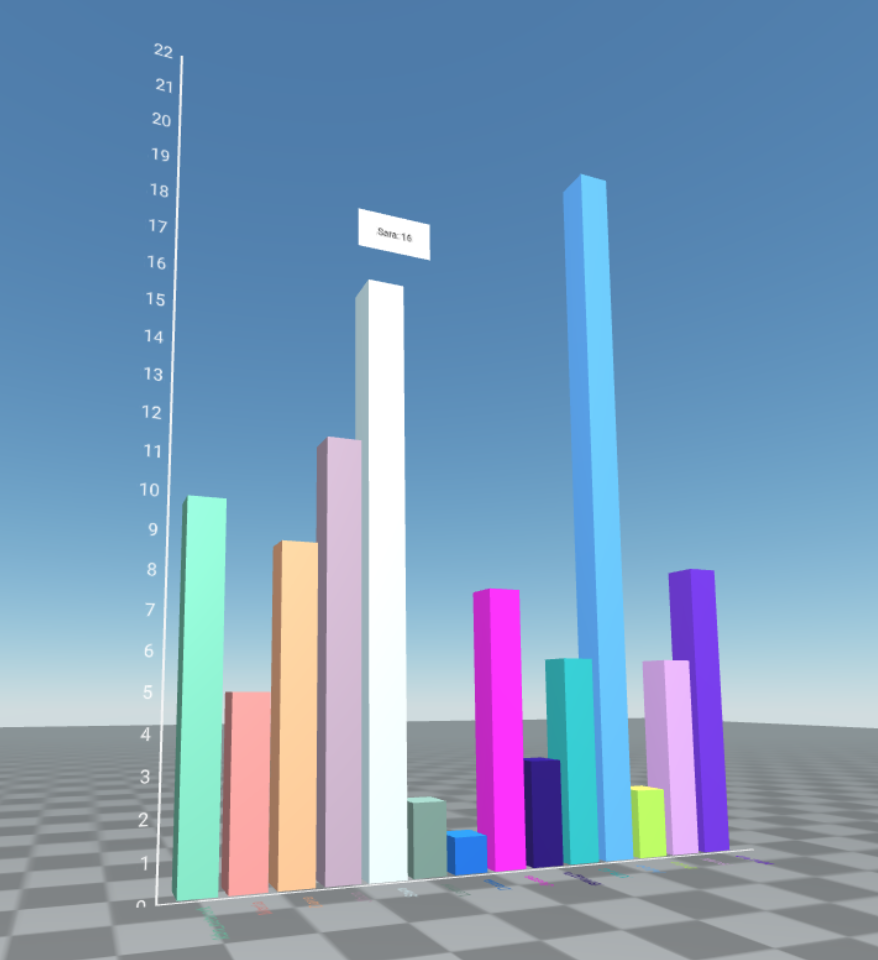
\includegraphics[width=5cm, keepaspectratio]{img/development/babiaxr-simplebar.png}
  \caption{Geosimplebarchart}
  \label{fig:babiaxrgeosimplebarchart}
  \endminipage\hfill
  \minipage{0.32\textwidth}
  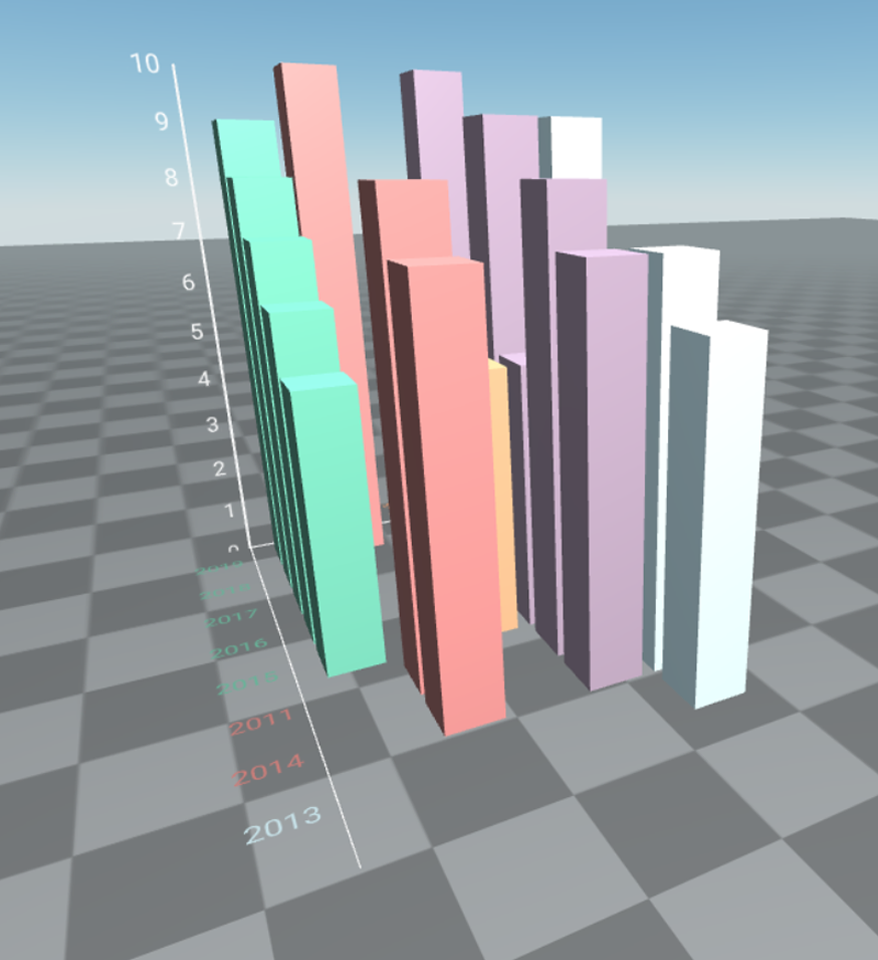
\includegraphics[width=5cm, keepaspectratio]{img/development/babiaxr-3dbar.png}
  \caption{Geo3dbarchart}
  \label{fig:babiaxrgeo3dbarchart}
  \endminipage\hfill
\end{figure}

\begin{figure}[H]
  \centering
  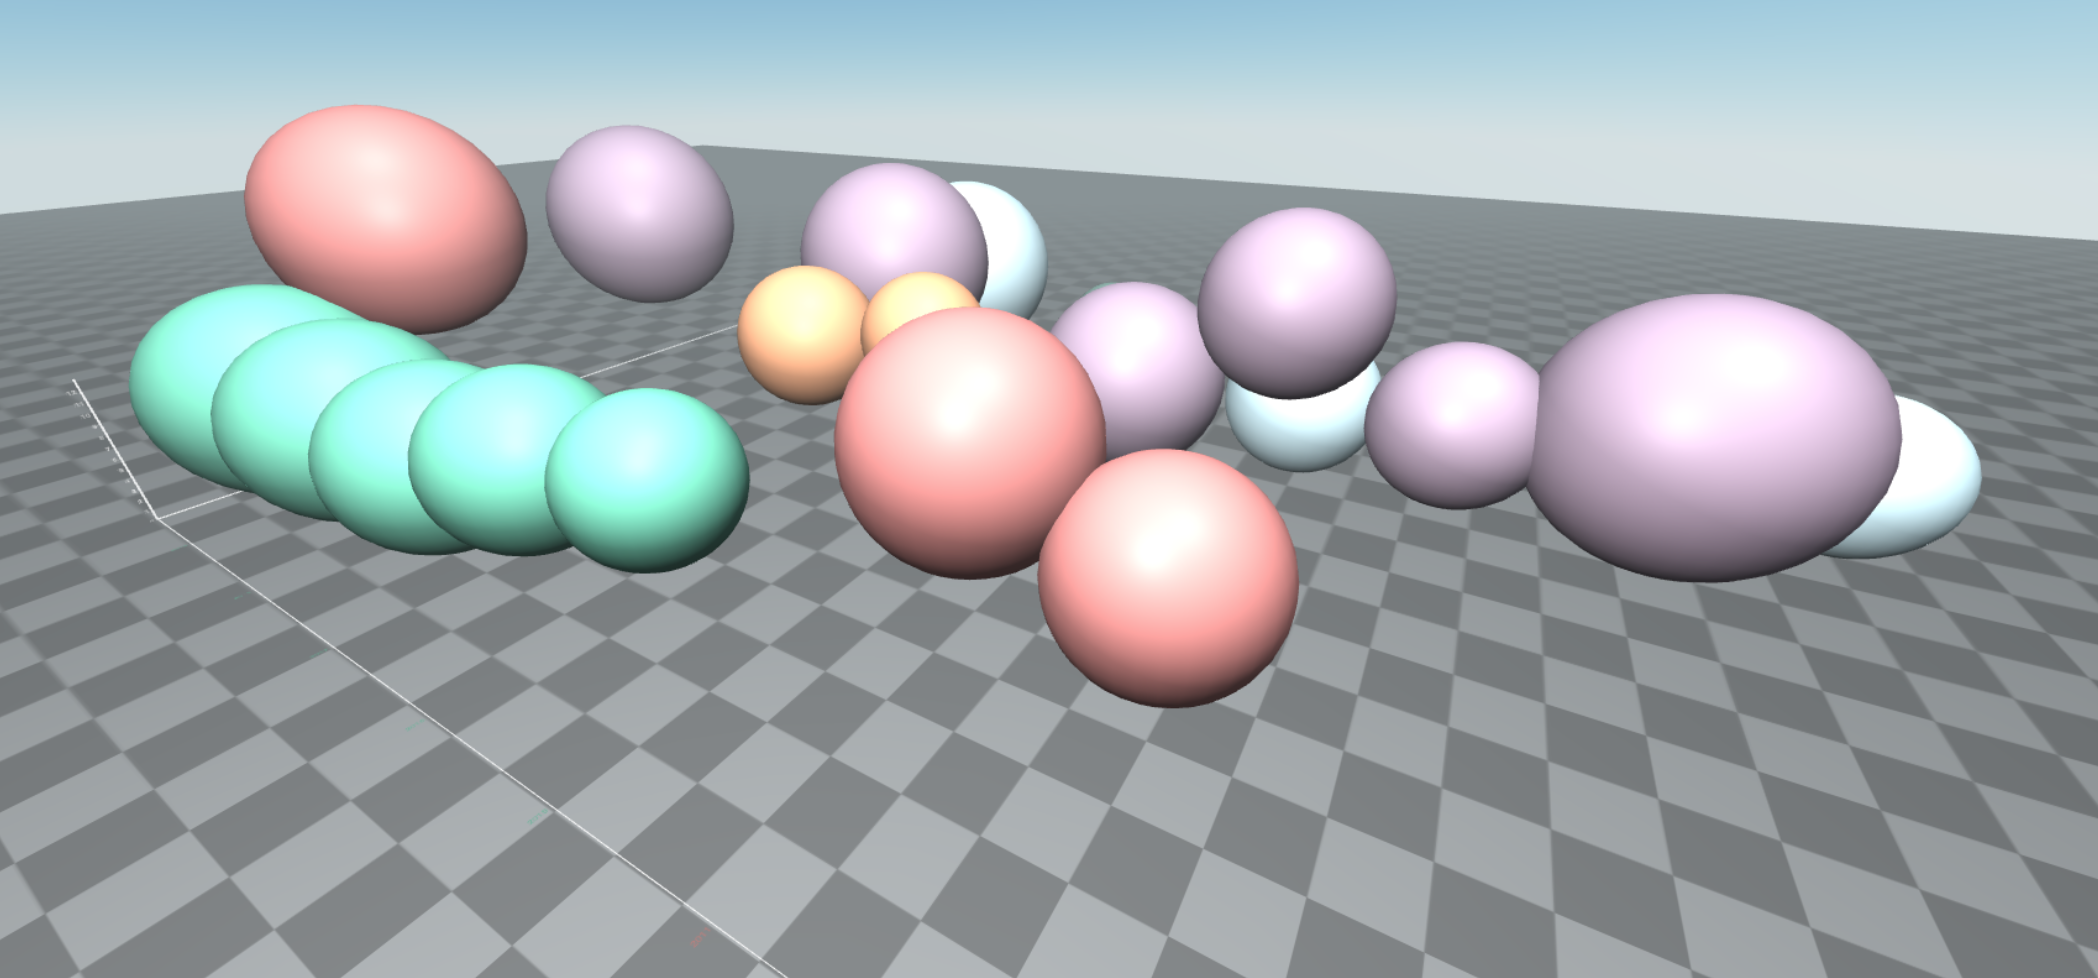
\includegraphics[width=10cm, keepaspectratio]{img/development/babiaxr-bubble.png}
  \caption{Geobubblechart}
  \label{fig:babiaxrgeobubblechart}
\end{figure}


Una vez que hemos visto lo que hace, probaremos a crear nuestro propio escenario con la componente “geopiechart” con datos que le daremos de forma manual. Para ello, nos apoyaremos en la documentación que nos facilita su autor.

\lstinputlisting[language=Html]{code/iteracion0-geopiechart.html}

Obteniendo como resultado:

\begin{figure}[H]
  \centering
  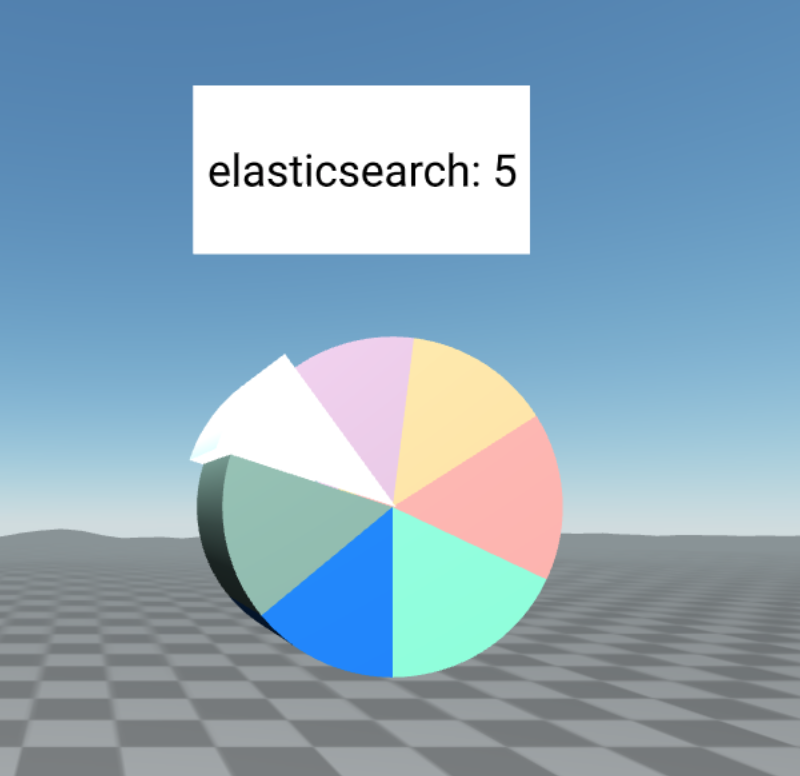
\includegraphics[width=6cm, keepaspectratio]{img/development/prueba-babiaxr.png}
  \caption{Pie Chart de Prueba}
  \label{fig:pruebababiaxr}
\end{figure}

Con todo esto, ya podemos proceder a crear nuestro primer plugin.


%%%%%%%%%%%
% SPRINT 1
%%%%%%%%%%%

\section{Sprint 1: Primeros Plugins de Visualización }
\label{sec:sprint1}

Ahora que conocemos las herramientas con las que trabajamos, es hora de ponernos a crear nuestro primer plugin. Esta parte es vital para el aprendizaje, así que iremos paso a paso.

Lo primero que haremos será crear un plugin simple, sin usar datos, que nos muestre un \textit{“Hola Mundo”} como visualización. Esto nos ayudará a conocer más en profundidad el funcionamiento  de la estructura anteriormente explicada.

Una vez que hayamos conseguido crear este primer plugin, intentaremos implementar una figura creada con A-Frame. Esto nos ayudará a entender cómo podemos añadir componentes A-Frame a nuestras visualizaciones.

También intentaremos crear un componente sencillo de A-Frame y lo implementaremos. Esto nos ayudará a entender cómo se han creado los componentes de BabiaXR.


%PLUGIN SIMPLE SIN DATOS
\subsection{Plugin Simple sin Datos}
\label{sec:holamundo}
Anteriormente en el capítulo \ref{sec:entorno}  explicamos cómo era la estructura base para crear plugins para Kibana. Iremos parte por parte hasta conseguir tener una visualización que simplemente nos muestre un \textit{“Hola Mundo”}.

A este primer plugin lo llamaremos \textit{hello-world-vis} y comenzaremos a programar los primeros archivos que nos permitirá registrar el plugin e instalar las dependencias npm que necesitamos.

\lstinputlisting[language=json]{code/iteracion1-package.json}

Parámetros utilizados:
\begin{itemize}
    \item \underline{name}: nombre del plugin.
    \item \underline{version}: versión de nuestro plugin.
    \item \underline{kibana}: versión de Kibana.
\end{itemize}

Como solo es una versión de prueba, únicamente indicaremos el nombre del plugin, la versión y para que version de Kibana es. Esta última se debe indicar bien, sino no funcionará. Por eso, como estamos desarrollando para la version 7.6, esto tiene que venir reflejado en nuestro \textit{package.json}. En esta ocasión, al ser un simple \textit{hola-mundo} no necesitaremos instalar ninguna dependencia.

Ahora procederemos a registrar nuestro plugin en \textit{index.js}:

\lstinputlisting[language=Javascript]{code/iteracion1-index.js}

Parámetros utilizados:
\begin{itemize}
    \item \underline{uiExports}: indica que el tipo de modulo vamos a exportar. Dentro de esta existen varios tipos: (\textit{hacks, visTypes, fieldformats, etc}).
    \item \underline{vis\_Types}: indicamos que el módulo que vamos a exportar se trata de un plugin de visualización.
\end{itemize}

Una vez dentro de \textit{vis\_Types} indicaremos el directorio donde se encuentra el archivo principal de nuestro plugin \textit{public/hello-world-vis.js}. Ahora pasaremos a crearlo. Al igual que para los plugins, las visualizaciones también deben registrarse. 

Lo primero que haremos será importar el paquete dentro de Kibana que nos permitirá registrar nuestra visualización. Debido a la migración que se está realizando en Kibana, la documentación que facilitaban y cualquier otro tutorial estaban obsoletos. Por lo que se tuvo que realizar una extensa búsqueda entre el repositorio de Kibana en Github y sus issues para ver cómo era la nueva forma de registrar las visualización. 

Al final, la mejor forma de averiguarlo fue inspeccionar dentro del código de Kibana y ver cómo registraban las visualizaciones que vienen de forma predeterminada en el cliente de Kibana. Esta se encuentra en el fichero \textit{kibana/src/legacy/core\_plugins/kbn\_vislib\_vis\_types/public/
kbn\_vislib\_vis\_types.js}\footnote{\url{https://github.com/elastic/kibana/blob/7.6}}, y la usaremos de base para la forma de registrar nuestras futuras visualizaciones.

Con esto, ya podemos importar el paquete que nos permitirá registrar la visualización:

\lstinputlisting[language=Javascript]{code/iteracion1-hello-world1.js}

Ahora pasaremos a definir nuestra visualización:
\lstinputlisting[language=Javascript]{code/iteracion1-hello-world2.js}

Parámetros utilizados:
\begin{itemize}
    \item \underline{name}: nombre de nuestra visualización.
    \item \underline{title}: título que aparecerá en el menú para elegir nueva visualización.
    \item \underline{icon}: icono que aparecerá en dicho menú.
    \item \underline{description}:  descripción que aparecerá en dicho menú.
    \item \underline{visualization}: indicaremos el controlador que usaremos en la visualización, éste lo crearemos a continuación para exportarlo.
    \item \underline{editor}: añade el editor, pero como por ahora no nos interesa, lo dejaremos en ‘default’.
\end{itemize}

Y por último, registramos la visualización:

\lstinputlisting[language=Javascript]{code/iteracion1-hello-world3.js}

Ya tenemos registrada nuestra primera visualización. Lo que le sigue es crear el controlador donde estará toda la parte lógica de nuestro plugin, pero antes de comenzar con ella vamos a crear un pequeño template \textit{public/index.html}, con el contenido de la visualización, que no es más que un \textit{“Hola Mundo”}.

\lstinputlisting[language=Html]{code/iteracion1-hola-mundo.html}

Listo esto, comenzamos a crear nuestro controlador \textit{public/hello-world-controller.js}. Lo primero que haremos será importar nuestro template.

\lstinputlisting[language=Javascript]{code/iteracion1-hello-world-controller1.js}

Este controlador es una clase con su correspondiente constructor; pero también necesitará las funciones de \textit{render()} y \textit{destroy()} para funcionar. Comenzamos creando el constructor:

\lstinputlisting[language=Javascript]{code/iteracion1-hello-world-controller2.js}

Lo único que hacemos es coger las variables \textit{el} y \textit{vis} y crear un \textit{container}:

\begin{itemize}
    \item \underline{el}: contenido de la visualización.
    \item \underline{vis}: contiene los parámetros que se crean al registrar la visualización.
    \item \underline{container}: en este contenedor añadiremos todo lo que queremos que muestre la visualización.
\end{itemize}

A continuación crearemos la función \textit{destroy()} que destruirá la visualización cada vez que salimos de la visualización o cada vez que actualizamos los datos que se van a mostrar en la visualización.

\lstinputlisting[language=Javascript]{code/iteracion1-hello-world-controller3.js}

Y por último, creamos la función \textit{render()}.

\lstinputlisting[language=Javascript]{code/iteracion1-hello-world-controller4.js}

Como Kibana es un cliente que permite monitorizar los datos almacenados en Elasticsearch, al crear un visualización se espera que Kibana realice una petición a Elasticsearch con los datos que quiere mostrar; y éste los devuelva. Estos datos vienen en dentro de la variable \textit{visData}; por tanto actualizaremos nuestra visualización cada vez que recibamos datos, aunque en esta ocasión los datos estarán en blanco. 
Lo único que haremos es meter el template que anteriormente hemos creado en el container de la visualización.

El siguiente paso es exportar el controlador:

\lstinputlisting[language=Javascript]{code/iteracion1-hello-world-controller5.js}

E importarlo en \textit{public/hello-world-vis.js}:

\lstinputlisting[language=Javascript]{code/iteracion1-hello-world4.js}

Como resultado nos encontramos con que dentro de crear nueva visualización aparece nuestra visualización con su nombre, icono y descripción.

\begin{figure}[H]
  \centering
  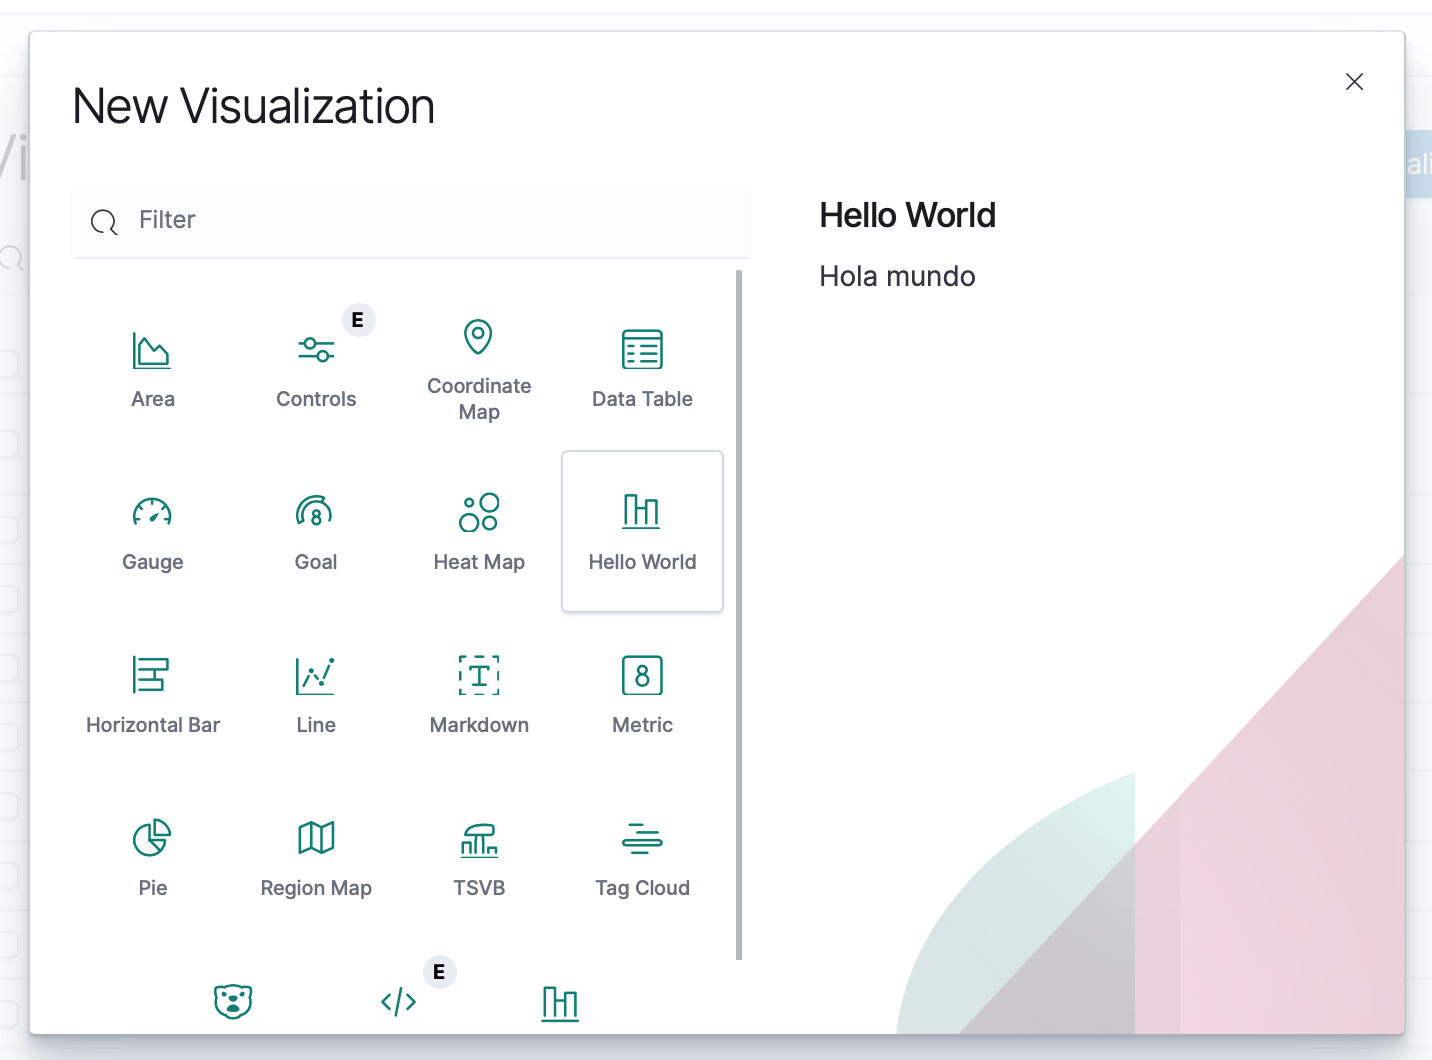
\includegraphics[width=10cm, keepaspectratio]{img/development/menu-visualizaciones.png}
  \caption{Menú con la nueva visualización}
  \label{fig:menuvisualization}
\end{figure}

Y obteniendo como resultado nuestra visualización \textit{¡Hola Mundo!}.

\begin{figure}[H]
  \centering
  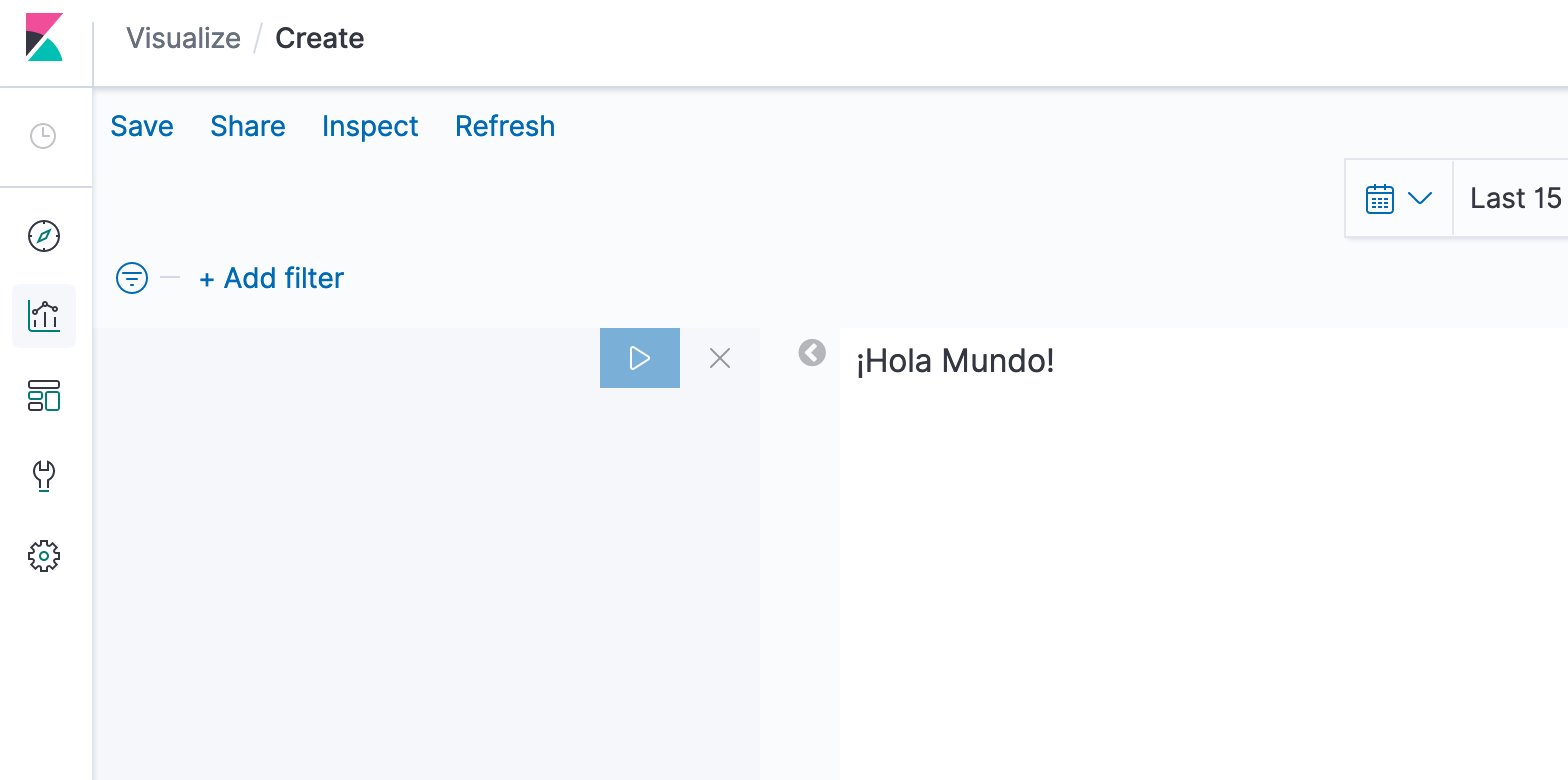
\includegraphics[width=10cm, keepaspectratio]{img/development/resultado-hola-mundo.png}
  \caption{Resultado Visualización Hola Mundo}
  \label{fig:resultadoholamundo}
\end{figure}



% IMPLEMENTACION A-Frame SIN DATOS
\subsection{Implementación de A-Frame sin Datos}
\label{sec:aframesindatos}

Una vez aprendidas las bases de cómo se crea un plugin de visualización para Kibana, el siguiente paso será conseguir integrar algún componente de la biblioteca de A-Frame para comprobar si estas dos tecnologías son compatibles entre sí.

En esta situación crearemos una visualización, tomando como base el plugin \textit{hello-world-vis} que creamos anteriormente; y le intentaremos añadir un componente primitivo de la biblioteca de A-Frame (por ejemplo, un cubo).

Para esto, necesitaremos tener instalado previamente el módulo NPM de A-Frame. Esto se consigue añadiendo las dependencias en \textit{package.json}.

\lstinputlisting[language=Json]{code/iteracion1-package2.json}

Y  para instalarlo usaremos el comando \textit{“npm install”} dentro del directorio que contiene nuestro \textit{package.json}.

Una vez que hemos descargado e instalado el módulo de A-Frame, lo declaramos en el controlador de la visualización \textit{hello-world-controller.js} para que podamos usarlo en el template.

\lstinputlisting[language=Javascript]{code/iteracion1-hello-world-controller5.js}

Y modificamos el HTML del template \textit{index.html} para que dibuje un cubo con A-Frame. Para ello, debemos conocer al menos estas dos etiquetas: 

\begin{itemize}
    \item \underline{a-scene}: permite manejar elementos creados con THREE.js y WebXR. Todos estos elementos deben estar contenido en esta etiqueta, sino no funcionará. Salvo que se le declare, creará por defecto la cámara y las luces.
    \item \underline{a-box}: crea un componente cubo en 3D según los atributos que le indiquemos.
\end{itemize}

\lstinputlisting[language=Html]{code/iteracion1-hola-mundo2.html}

Obteniendo como resultando la siguiente visualización:

\begin{figure}[H]
  \centering
  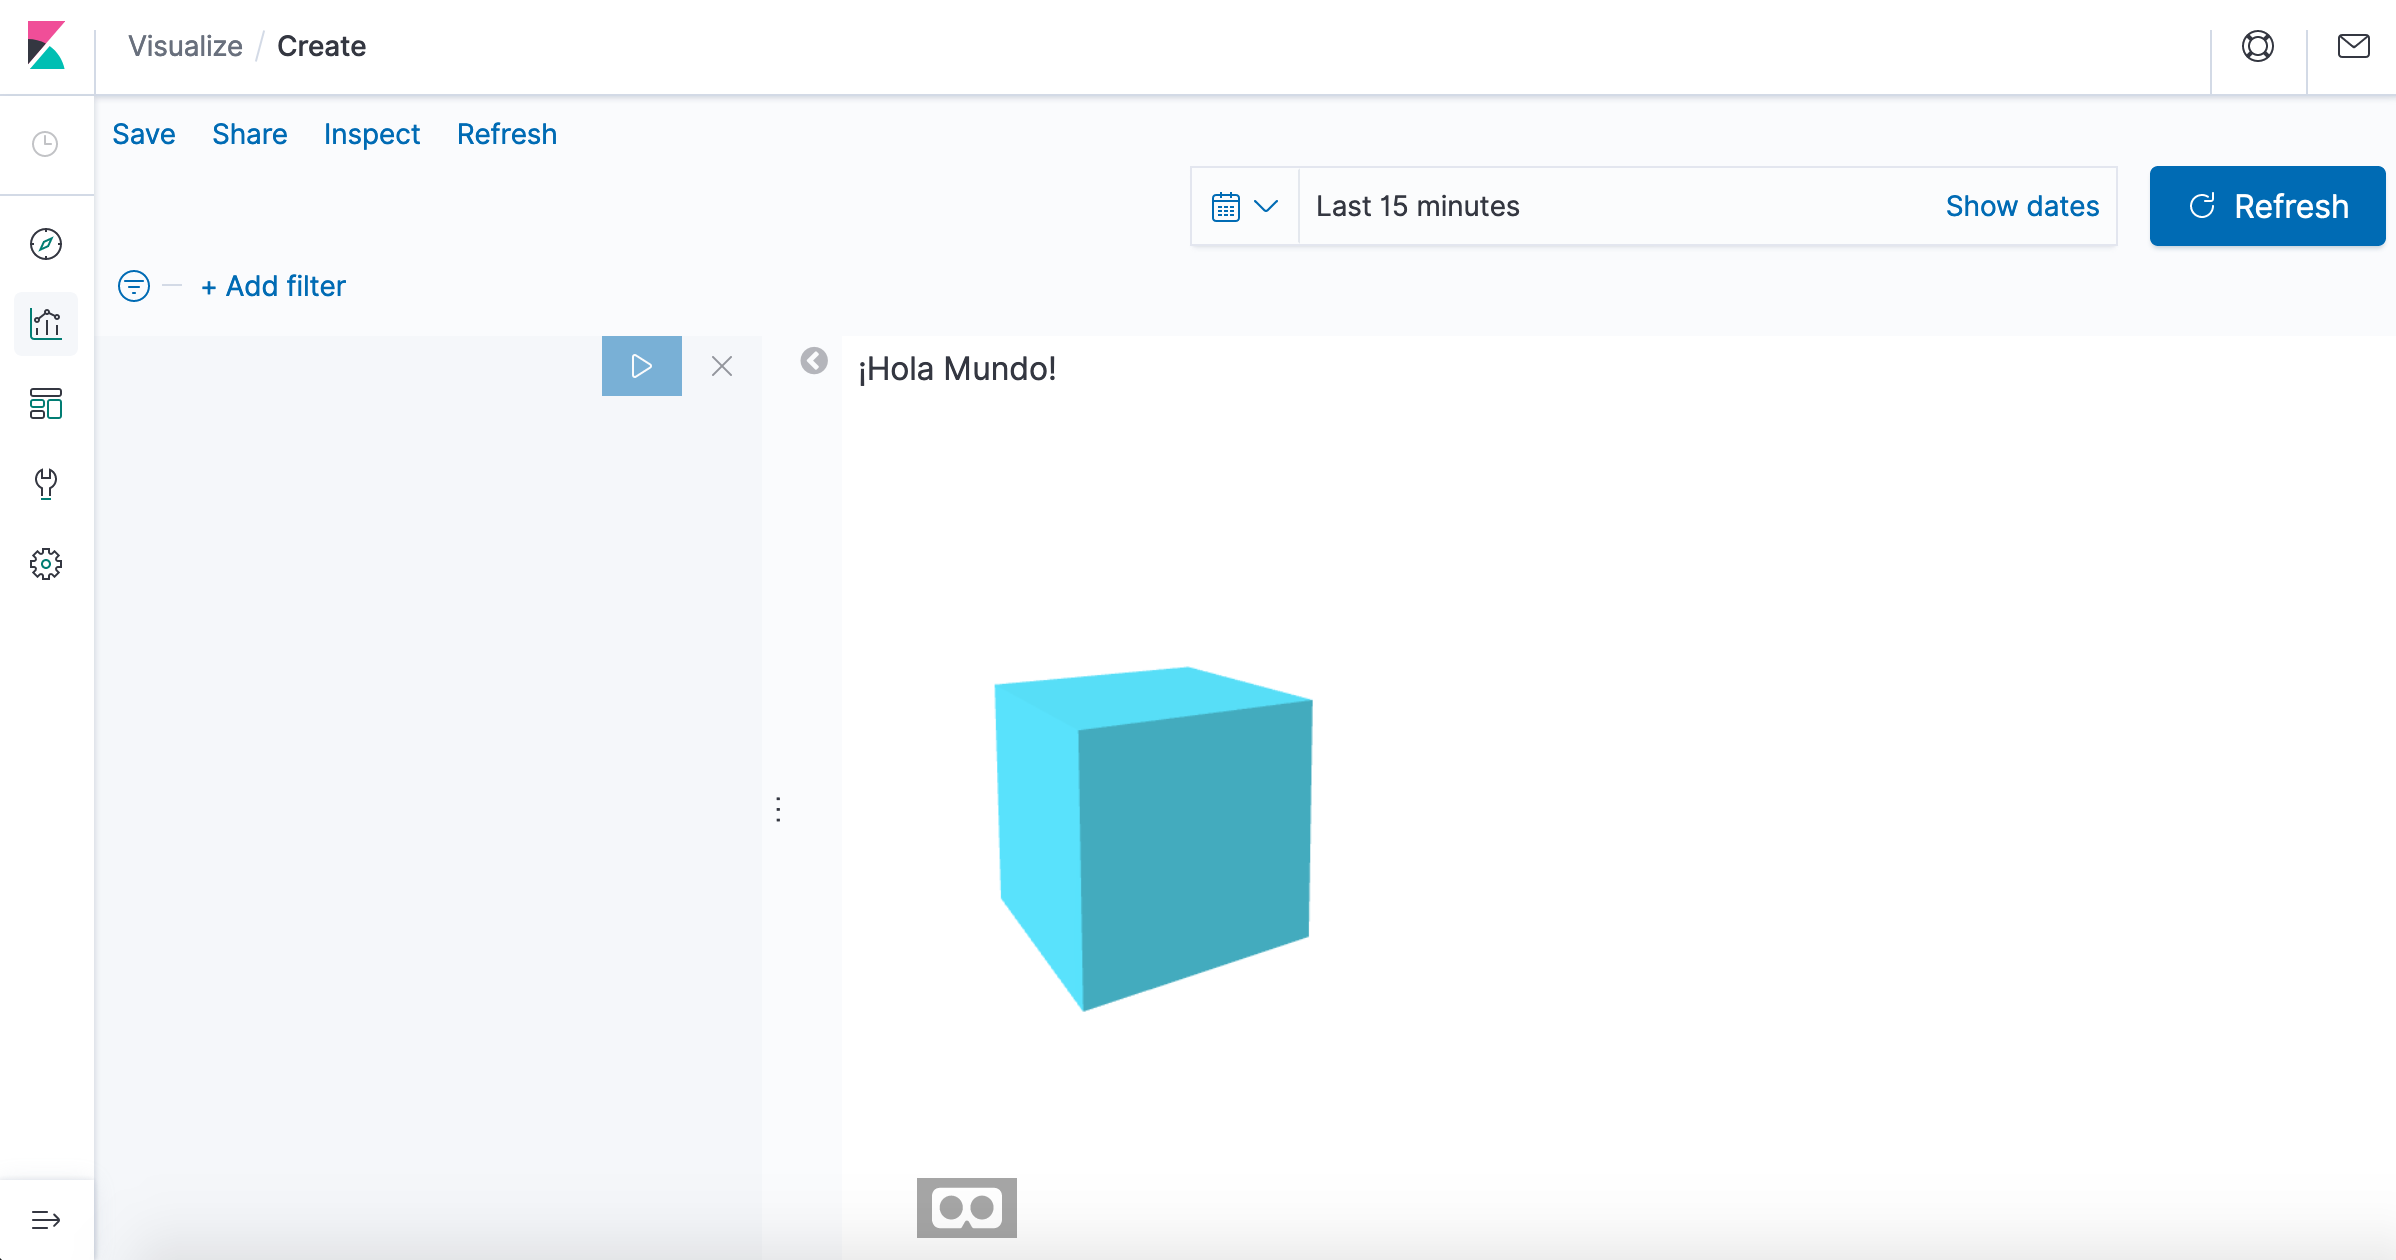
\includegraphics[width=10cm, keepaspectratio]{img/development/resultado-aframe-box.png}
  \caption{Resultado Visualización de cubo con A-Frame son Datos}
  \label{fig:resultadoaframesindatos}
\end{figure}

Con esto podemos asegurar que Kibana soporta visualizaciones creadas con la biblioteca A-Frame.




% CREACION COMPONENTE A-Frame
\subsection{Creación de Componente A-Frame}

Ahora ya sabemos que Kibana nos permite usar A-Frame en sus visualizaciones, pero vamos a estudiarlo más en profundidad. Como se explicó anteriormente en el capítulo\ref{sec:babiaxr}, BabiaXR es una biblioteca de componente creadas con A-Frame; por lo que en esta ocasión se creará un componente A-Frame para entender mejor el funcionamiento interno de BabiaXR.

Ya que hemos creado un cubo como componente primitivo, esta vez lo sustituiremos por otro cubo; pero creado por este método tomando como referencia el ejemplo que nos facilita la documentación de A-Frame \footnote{\url{https://aframe.io/docs/1.0.0/introduction/writing-a-component.html}}. 

El primer paso es crear un fichero que se llamará \textit{box.js} y registrar el componente de la siguiente esquema:

\lstinputlisting[language=Javascript]{code/iteracion1-box1.js}

Los parámetros que le indicamos en el constructor son las propiedades que, más adelante, indicaremos dentro de las etiquetas del HTML.

Estas componentes funcionan como clases y deben contener ciertas funciones para que se puedan renderizar: \textit{init()}, \textit{update()} y \textit{destroy()}.

Comenzaremos creando la función \textit{init()}:

\lstinputlisting[language=Javascript]{code/iteracion1-box2.js}

Esta función inicializa la geometría, material y malla del componente a partir de los parámetros que recibe cuando se declaran en el HTML. Para luego renderizar la figura inicializada.

La función \textit{update()} se ejecutará cuando algún dato cambia. En este caso no lo vamos a necesitar pero como más adelante vamos a extraer datos de Elasticsearch para modificar el componente, lo creamos.

\lstinputlisting[language=Javascript]{code/iteracion1-box3.js}

Esta función lo que hará será modificar nuestro cubo con los nuevos valores recibidos.

Y por último, creamos la función \textit{destroy()} que borrará la figura en el momento de cerrar la visualización.

\lstinputlisting[language=Javascript]{code/iteracion1-box4.js}

Ahora que ya tenemos creada una componente propia, lo que sigue es declararla en nuestro controlador.

\lstinputlisting[language=Javascript]{code/iteracion1-hello-world-controller7.js}

Y modificaremos el template para que nos dibuje un cubo creado con nuestra componente; y le añadiremos también una esfera con la etiqueta \textit{<<a-sphere>>} para ver que se pueden mezclar componentes primitivas de A-Frame con componente creadas por otros usuarios. 

Para insertar estas componentes, que no vienen de forma pre-determinadas por A-Frame, usaremos la etiqueta \textit{<<a-entity>>} seguido del atributo con el nombre de la componente tal y como se ha registrado. En nuestro caso \textit{<<a-entity box>><</a-entity>>}. Después, añadimos el resto de atributos, al igual que hicimos con el cubo anteriormente en el capítulo \ref{sec:aframesindatos}

\lstinputlisting[language=Html]{code/iteracion1-hola-mundo3.html}

Una de las complicaciones que no se mencionaron anteriormente fue que la escena se salía de la visualización de Kibana. Añadiendo el atributo \textit{embedded} a la escena corregimos este error; pero para asegurarnos haremos una pequeña hoja de estilos para que el \textit{<<div>>} de nuestra visualización no se salga, la cual llamaremos \textit{hello-world.less}.

\lstinputlisting[language=Html]{code/iteracion1-hello-world.less}

E importamos esta hoja de estilo dentro del controlador de la visualización.

\lstinputlisting[language=Javascript]{code/iteracion1-hello-world-controller8.js}

Obteniendo como resultado la siguiente visualización:

\begin{figure}[H]
  \centering
  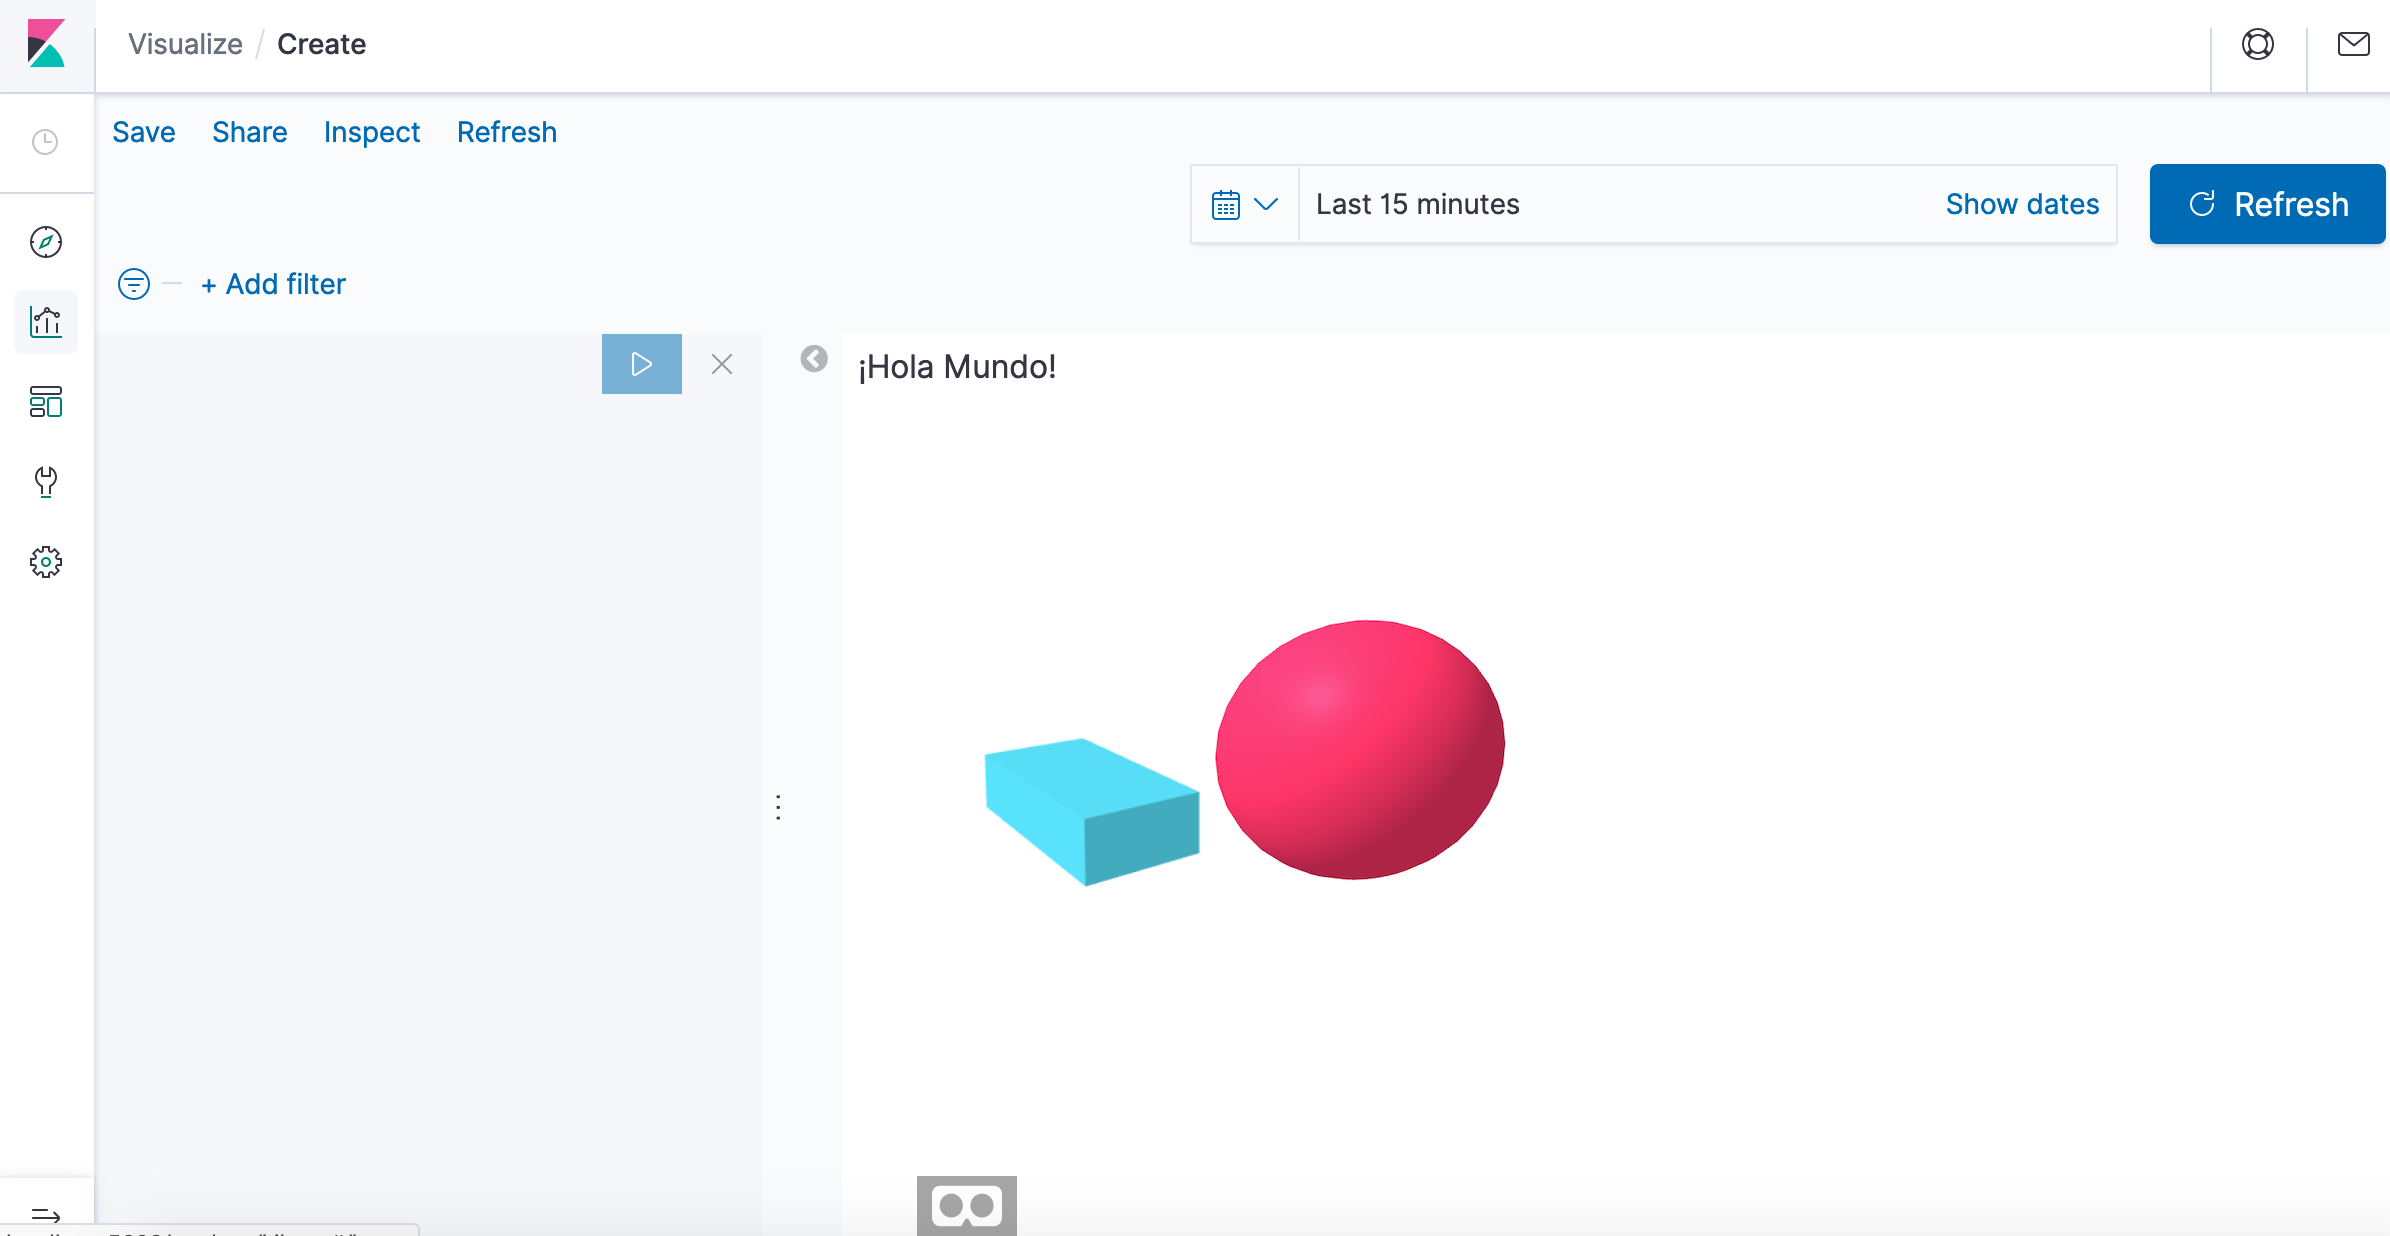
\includegraphics[width=10cm, keepaspectratio]{img/development/resultado-componente-box.png}
  \caption{Resultado Visualización de Componente Cubo con Esfera de A-Frame sin Datos}
  \label{fig:resultadocomponente}
\end{figure}




%%%%%%%%%%%
% SPRINT 2
%%%%%%%%%%%

\section{Sprint 2: Visualización con datos Elasticseach }
\label{sec:sprint2}

Hasta este punto hemos aprendido a crear un plugin simple para Kibana e integrarlo con A-Frame. El siguiente paso será aprender a sacar datos de Elasticsearch y poder dibujar un figura de aframe, en este caso un cubo, con las dimensiones que le obtenemos de dichos datos. Para ello, seguiremos los siguiente pasos:
\begin{enumerate}
    \item Añadir Editor y Schemas.
    \item Construir Visualización que muestre datos.
    \item Integración de Aframe con datos.
\end{enumerate}

%EDITOR Y SCHEMAS
\subsection{Editor y Schemas}
\label{sec:schemas}

Antes de ponernos a crear una nueva visualización donde nos muestre datos de Elasticsearch, necesitamos un editor que nos permita seleccionar los datos que queremos mostrar. 

Comenzaremos creando el diseño de nuestro editor. Kibana nos permite seleccionar dos tipo de datos: \textit{metrics} y \textit{buckets}.
\begin{itemize}
    \item \underline{metrics}: hace referencia a datos que se pueden calcular, por ejemplo, media, máximo, sumatorio, etc.
    \item \underline{buckets}: refiere a un conjunto de datos que no se pueden calcular, por ejemplo, fechas, sucursales, tipos, etc.
\end{itemize}

Como el objetivo final de este sprint es crear una visualización que nos muestre un cubo, determinamos que necesitaremos 3 datos metrics que serán los datos que usaremos para crear las dimensiones del cubo que dibujaremos más adelante.

Estos datos vienen estructurados dentro de \textit{Schemas} que el propio Kibana permite declarar a la hora de crear la visualización para luego registrarla. Para ello, añadiremos las siguiente líneas en \textit{hello-world-vis.js}:

Antes de nada, importamos los correspondientes paquetes que nos permite declarar los schemas e indicar el tipo de dato que vamos a usar, en este caso metrics.


\lstinputlisting[language=Javascript]{code/iteracion2-hello-world-vis1.js}


Una vez importado, añadiremos nuevos parámetros de nuestro editor dentro de la constante \textit{helloWorldDefinition}:

\lstinputlisting[language=Javascript]{code/iteracion2-hello-world-vis2.js}


Parámetros utilizados:
\begin{itemize}
    \item \underline{group}: indica el tipo de dato: metric o bucket.
    \item \underline{name}: nombre que recibirá el dato.
    \item \underline{title}: el título que mostrará en el editor.
    \item \underline{min}: indica el mínimo de datos que tenemos usar.
    \item \underline{max}: indica el máximo de datos que podemos usar.
    \item \underline{aggFilter}: aquí podemos indicarle qué tipos de dato, en este caso tipos de métricas, queremos usar.
\end{itemize}

Al instante de añadir esto, obtenemos como resultado un editor como el que vemos a continuación:

\begin{figure}[H]
  \centering
  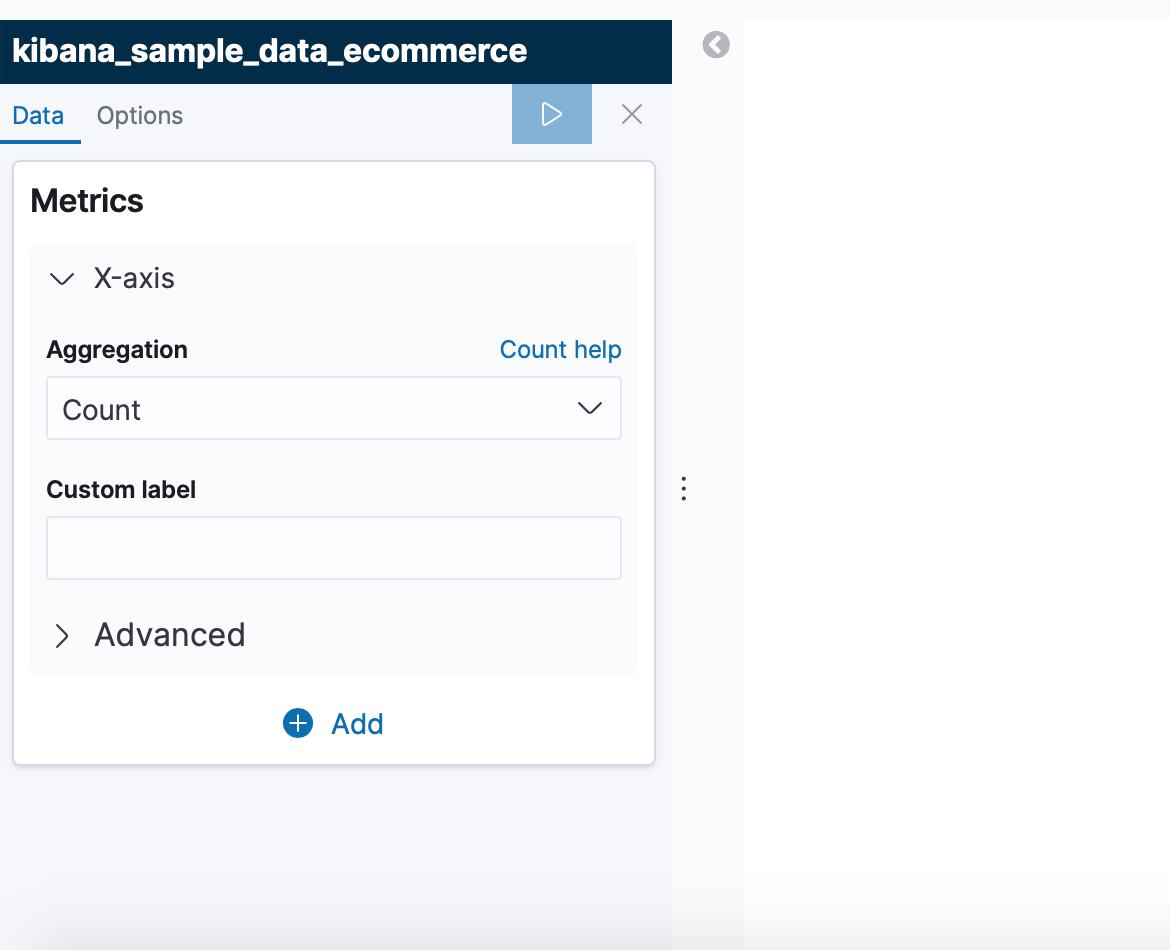
\includegraphics[width=9cm, keepaspectratio]{img/development/editor-resultado.png}
  \caption{Resultado del Editor}
  \label{fig:editor}
\end{figure}

%PLUGIN SIMPLE CON DATOS
\subsection{Plugin Simple con Datos}
\label{sec:holamundocondatos}

Ahora que ya podemos elegir los datos en el editor de Kibana, el siguiente paso es conseguir que la visualización muestre dichos datos de forma sencilla.

Para esto debemos haber aprendido, como se vió en el sprint anterior (capítulo \ref{sec:sprint1}), el funcionamiento de creación y renderizado para entender dónde Kibana recibe los datos de Elasticsearch. Así que lo primero que tenemos que hacer es encontrar dónde recibimos los datos que pedimos con el editor.

Si revisamos el esquema del proceso de creación de una visualización en el capítulo \ref{sec:holamundo}, podemos suponer que los datos que recibimos vendrán en la variable \textit{visData}. Lo comprobaremos de la siguiente forma:

\lstinputlisting[language=Javascript]{code/iteracion2-hello-world-controller1.js}

Con esto podremos ver que datos recibimos en la consola del navegador.

\begin{figure}[H]
  \centering
  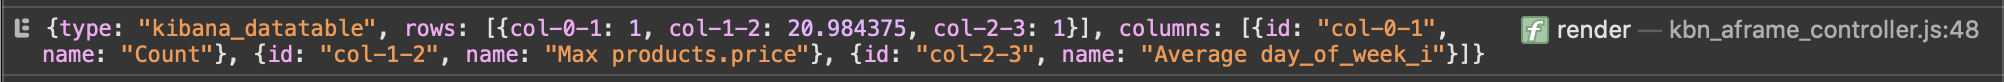
\includegraphics[width=16cm, keepaspectratio]{img/development/captura-visData.png}
  \caption{Captura de visData en la consola}
  \label{fig:visData}
\end{figure}

Esto nos sirve para analizar en cómo es el formato de los datos recibidos de Elasticsearch, para luego extraer los datos que nos interesa mostrar. 

En primer lugar, vemos que se divide en 3 registros: 
\begin{itemize}
    \item \underline{type}: tipo del archivo. En este caso, kibana\_datatable.
    \item \underline{rows}: contiene únicamente los datos obtenidos en formato registro en la que la clave con la forma \textit{col-X-X} que indica la posición; y el valor con el dato obtenido.
    \item \underline{columns}: contiene las etiquetas que hacen referencia a los datos obtenidos. Vienen en forma de array de registros, donde \textit{id} indica la posición del dato; y \textit{name} indica el nombre del valor. 
\end{itemize}

Analizando todo esto sacaremos los datos, con sus nombres, para guardarlo en la variable \textit{metrics}.

\lstinputlisting[language=Javascript]{code/iteracion2-hello-world-controller2.js}

Tras esto, lo añadimos a la visualización, de forma simple, de la siguiente forma:


\lstinputlisting[language=Javascript]{code/iteracion2-hello-world-controller3.js}


Como resultado obtenemos las figuras, que agregamos anteriormente en el capítulo anterior, seguido de los 3 valores que pedimos desde el editor.

\begin{figure}[H]
  \centering
  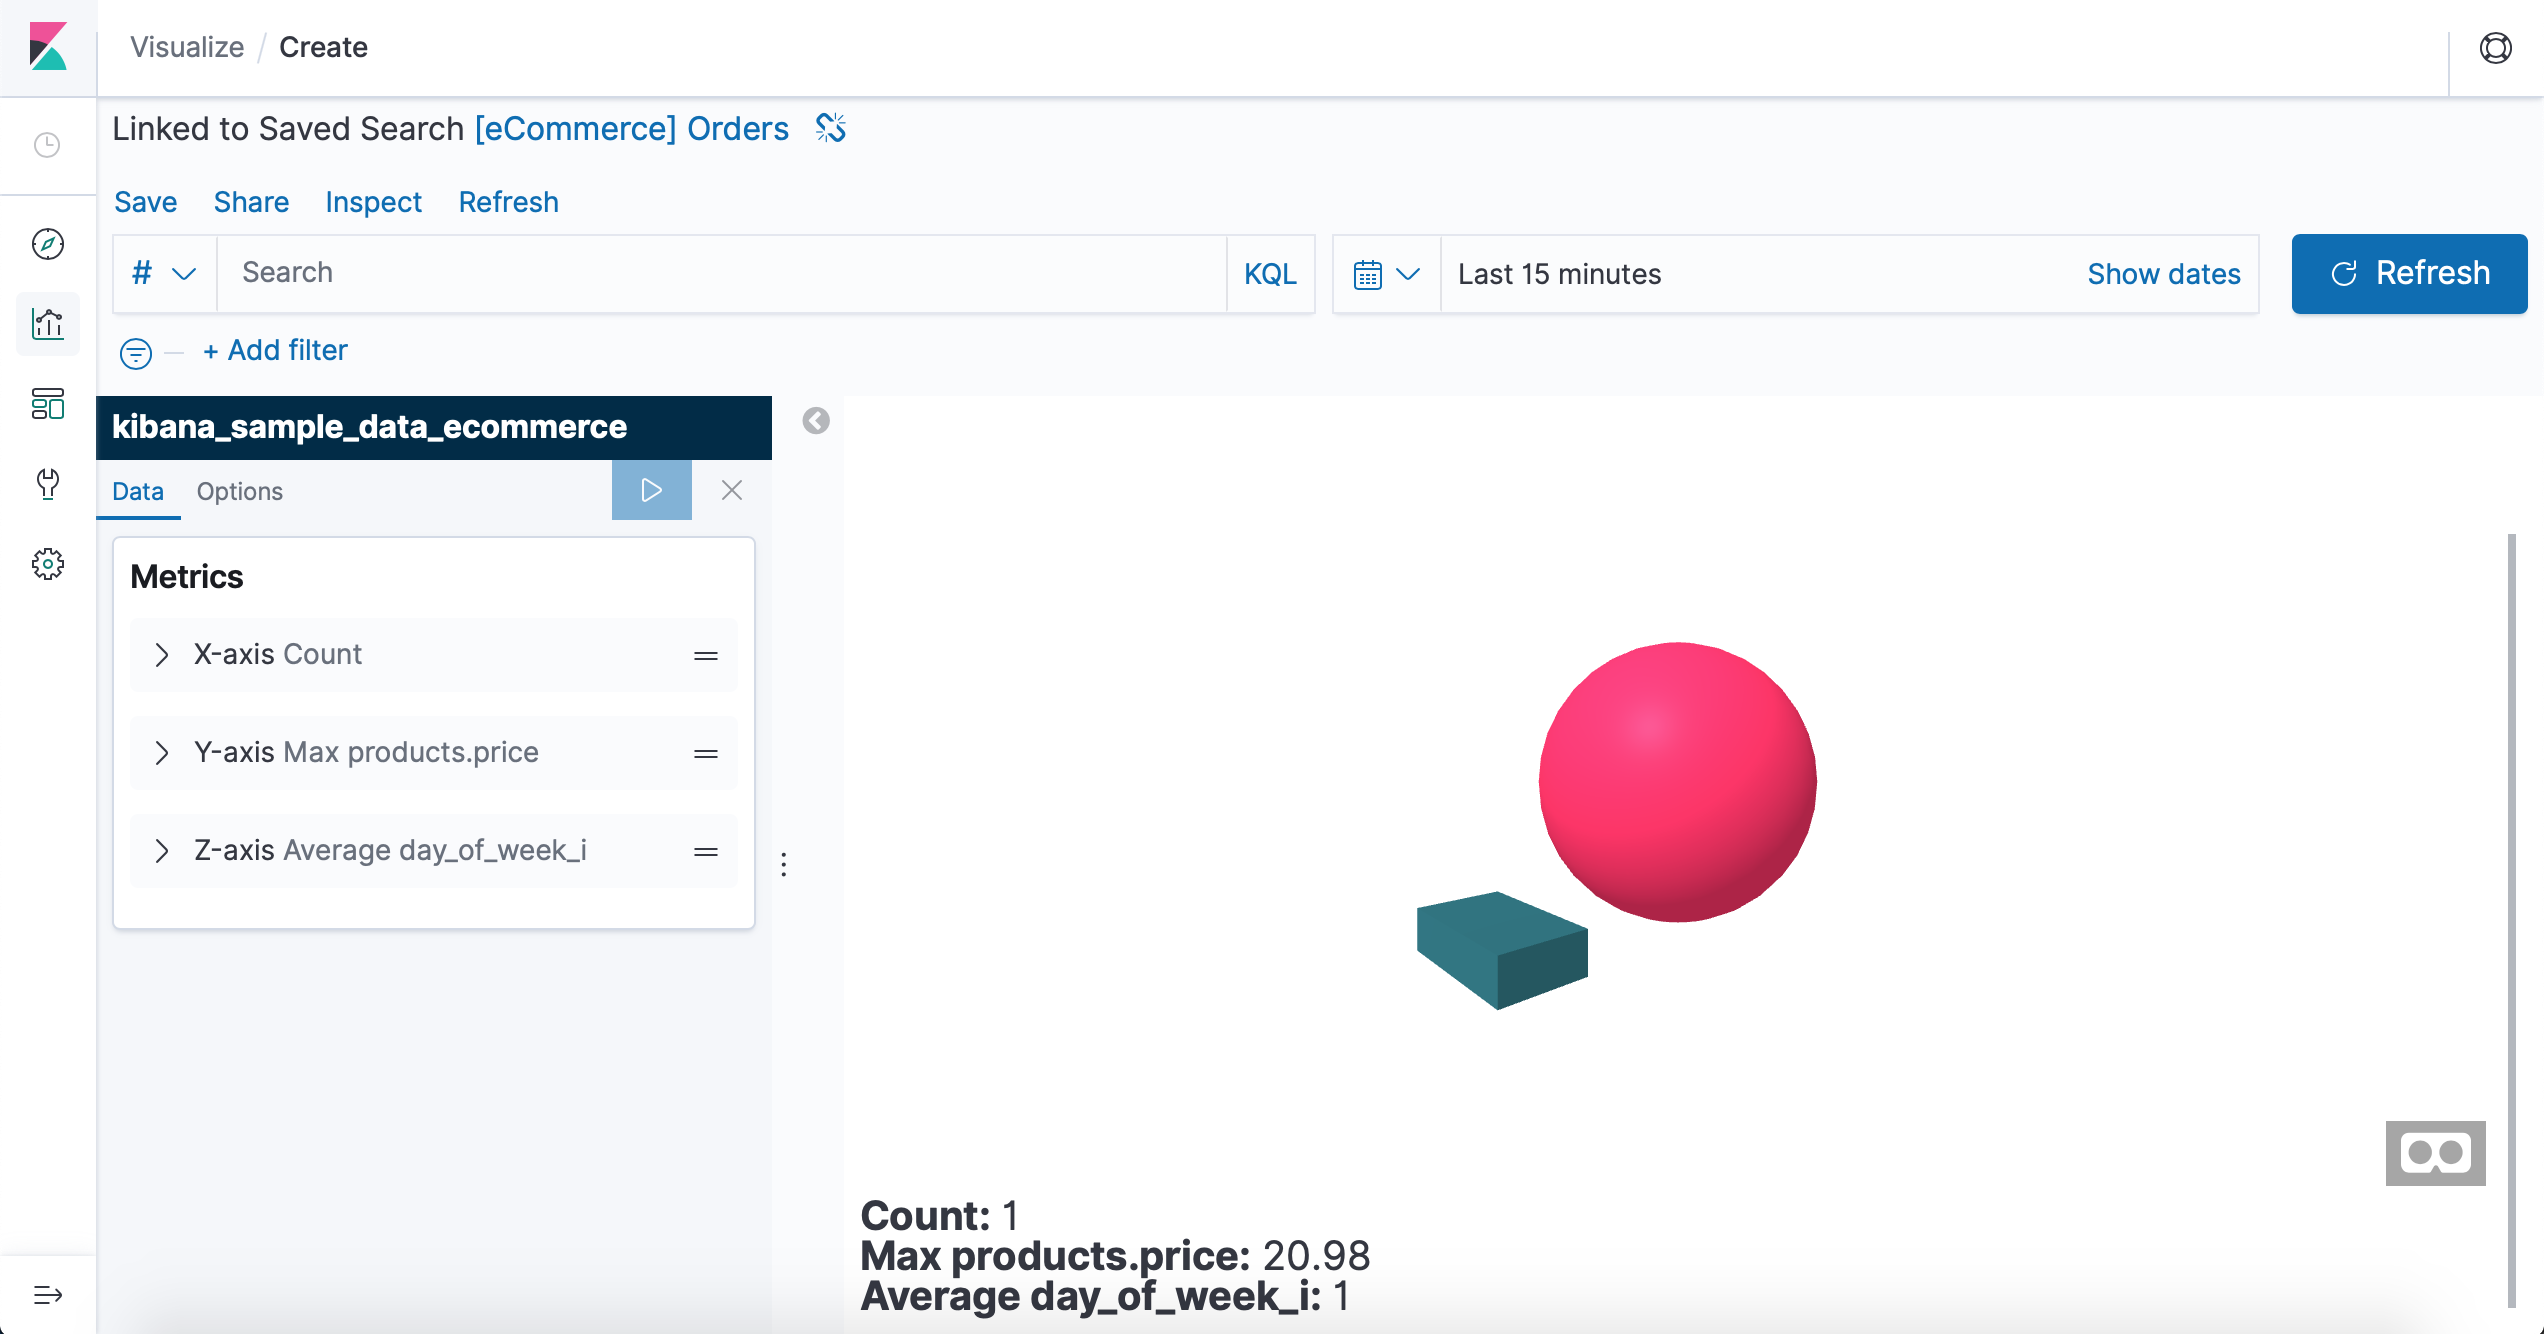
\includegraphics[width=10cm, keepaspectratio]{img/development/resultado-simple-data.png}
  \caption{Resultado Visualización con Datos}
  \label{fig:simplewithdata}
\end{figure}


%A-RAME CON DATOS
\subsection{Integración de A-Frame con datos}
\label{sec:aframecondatos}

Ahora que ya hemos aprendido a obtener los datos que pedimos a Elasticsearch para incluirlos en nuestra visualización, el siguiente paso es saber añadir estos datos para poder crear las figuras en base a estos datos.

Únicamente nos centraremos en crear el cubo tomando como valores las 3 métricas que pedimos desde el editor. Para ello, tenemos dos opciones:

\begin{enumerate}
    \item Insertar los datos al HTML usando AngularJS.
    \item Crear la figura directamente desde el controller usando A-Frame con Javascript. \footnote{\url{https://aframe.io/docs/1.0.0/introduction/javascript-events-dom-apis.html#retrieving-component-data-with-getattribute}}
\end{enumerate}

Analizando un poco como Kibana crea sus visualizaciones predeterminadas, creo que la mejor opción es la segunda y así nos ahorramos tener que usar más bibliotecas.

Por eso, eliminaremos el archivo \textit{index.html}, eliminamos la línea donde importamos dicho archivo y cambiamos la siguiente línea de \textit{render()}:

\lstinputlisting[language=Javascript]{code/iteracion2-hello-world-controller4.js}

Ahora crearemos el escenario justo después de añadir las métricas obtenidas de Elasticsearch.

\lstinputlisting[language=Javascript]{code/iteracion2-hello-world-controller5.js}

El siguiente paso será añadir las figuras. Empezaremos por dibujar una esfera usando las primitivas que tiene A-Frame. Usaremos los mismos valores que teníamos en \textit{index.html} pero variando algún dato al gusto. Por el momento solo le añadimos los datos de forma manual porque lo único que queremos es probar cómo podemos crear una figura de esta forma.

Lo creamos de la siguiente forma:

\lstinputlisting[language=Javascript]{code/iteracion2-hello-world-controller6.js}

Esta última línea, añade la figura en el escenario anteriormente creado.

Ahora que está creado todo la escena con la figura, la añadimos el contenedor de la visualización para que nos la muestre en Kibana.

\lstinputlisting[language=Javascript]{code/iteracion2-hello-world-controller7.js}

Obteniendo como resultado la siguiente visualización.

\begin{figure}[H]
  \centering
  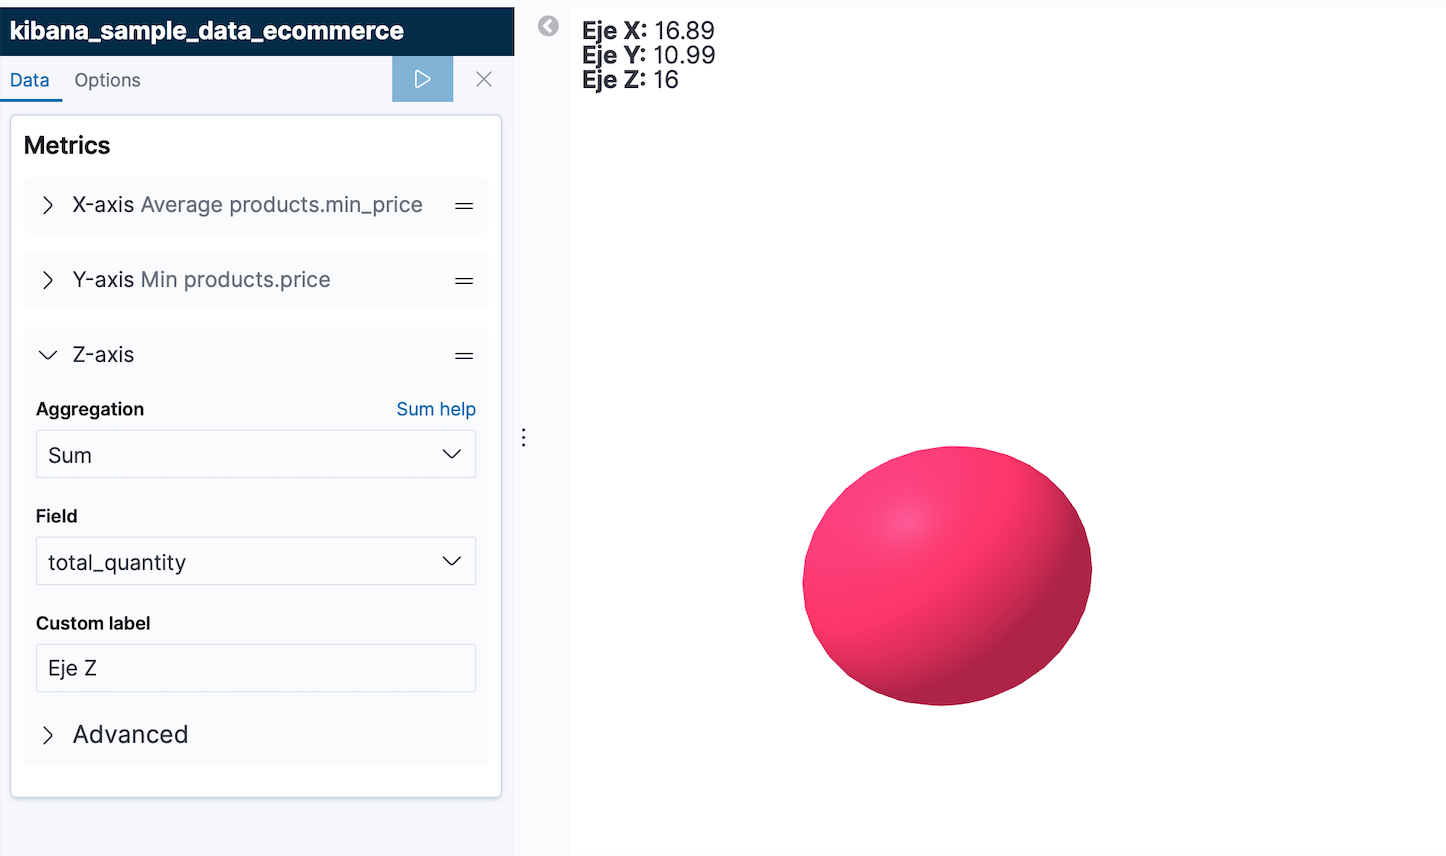
\includegraphics[width=10cm, keepaspectratio]{img/development/only_sphere.png}
  \caption{Esfera A-Frame con Javascript}
  \label{fig:onlysphere}
\end{figure}

Una vez hemos conseguido que nos dibuje la esfera, haremos el mismo procedimiento para crear el cubo pero con un par de variaciones:

\begin{enumerate}
    \item Usaremos el cubo que creamos por componente.
    \item Añadiremos los datos obtenidos de Elasticsearch.
\end{enumerate}

Como usaremos el componente, revisaremos que \textit{box.js} este importado en el controlador.

Ahora, declaramos un array con las dimensiones que vamos a usar para crear el cubo. 

\lstinputlisting[language=Javascript]{code/iteracion2-hello-world-controller8.js}

Y añadimos los valores en la variable axis tras añadirlo también en metrics.

\lstinputlisting[language=Javascript]{code/iteracion2-hello-world-controller9.js}

Por último, solo nos queda crear la figura de la misma forma y añadirlo en la escena:

\lstinputlisting[language=Javascript]{code/iteracion2-hello-world-controller10.js}

Como se ve, la diferencia con la esfera es que creamos un a-entity con el atributo \textit{`box'} y no \textit{`geometry'} y dándole los datos que declaramos en el constructor de \textit{box.js}.

Con esto, obtenemos como resultado un cubo que varía en base a los datos que le pedimos a Elasticsearch.

\begin{figure}[H]
  \centering
  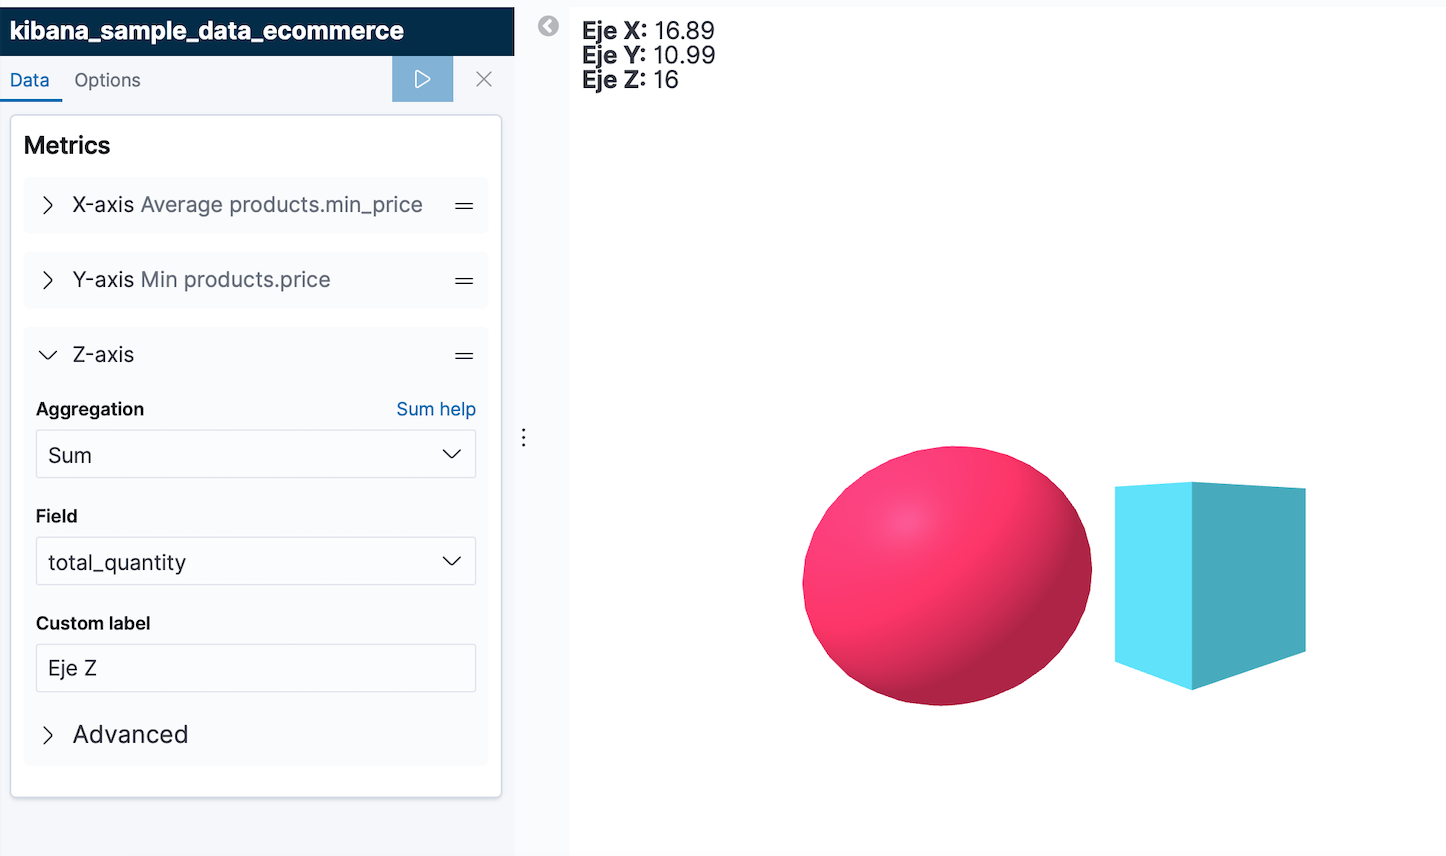
\includegraphics[width=10cm, keepaspectratio]{img/development/box_with_data.png}
  \caption{Resultado de integración de A-Frame con datos}
  \label{fig:boxwithdata}
\end{figure}


%%%%%%%%%%%
% SPRINT 3
%%%%%%%%%%%

\section{Sprint 3: Implementación de BabiaXR }
\label{sec:sprint3}

Tras haber completado toda la parte básica en cuanto a la creación de un plugin para Kibana y la integración de gráficos VR usando A-Frame, procederemos a integrar la biblioteca de BabiaXR. 

Como explicamos anteriormente (capítulo\ref{sec:babiaxr}) BabiaXR es una biblioteca de componentes donde cada componente es un tipo de gráfica y por tanto será un tipo de visualización de nuestro plugin.

Para este sprint, cogereremos un solo componente de BabiaXR y lo integraremos en nuestro plugin. El componente elegido será \textit{geopiechart} que nos creará un visualización que nos mostrará una gráfica de tipo pie. 

Al igual que hicimos en el anterior sprint, dividiremos el sprint en dos partes:

\begin{enumerate}
    \item Integraremos pie chart sin usar datos.
    \item Integraremos pie chart usando datos.
\end{enumerate}

% PIE CHART SIN DATOS
\subsection{Visualización Pie Chart sin Datos}
\label{sec:piewithoutdata}

Anteriormente estábamos trabajando con un plugin de prueba; pero como esta parte ya será parte del resultado final, crearemos un nuevo plugin, cogiendo como referencia nuestro plugin de prueba, y lo llamaremos \textit{kbn\_aframe}.

Para empezar, introducimos el nombre de nuestro nuevo plugin, además de agregarle el nombre del autor y las dependencias que necesitaremos. Como lo hemos hecho anteriormente, este va dentro de \textit{package.json}.

\lstinputlisting[language=Json]{code/iteracion3-package.json}

Dependencias que necesitamos:
\begin{itemize}
    \item \underline{aframe}: para que podamos crear componente hechas con A-Frame.
    \item \underline{aframe-babia-components}: biblioteca de componentes de A-Frame con las gráficas que vamos a implementar.
    \item \underline{aframe-extras}: componente de aframe que añade otros tipo de controles diferentes a los que vienen de base con A-Frame.
    \item \underline{aframe-environment-component}: componente de A-Frame que permite crear entornos visualmente más atractivos que el que viene de base en A-Frame.
\end{itemize}

También añadiremos el directorio de nuestro nuevo fichero principal, al que llamaremos \textit{kbn\_aframe.js}, dentro de \textit{index.js}.

\lstinputlisting[language=Javascript]{code/iteracion3-index.js}

Y declararemos nuestra nueva visualización para registrarla posteriormente.

\lstinputlisting[language=Javascript]{code/iteracion3-kbn_aframe1.js}

Ahora nos vamos al controlador, que hemos llamado \textit{kbn\_aframe\_controller.js}, y lo primero que haremos será importar las dependencias que hemos instalado anteriormente.

\lstinputlisting[language=Javascript]{code/iteracion3-kbn_aframe_controller1.js}

El siguiente paso es crear nuestra visualización dentro del render tomando como referencia el ejemplo que encontramos en la documentación de BabiaXR\footnote{\url{https://github.com/babiaxr/aframe-babia-components/blob/master/examples/charts/pie_chart/index.html}}. Para ello, lo dividiremos en varias partes:

\begin{enumerate}
    \item Crearemos el entorno y le añadiremos las luces de la escena.
    \item Añadiremos los datos de forma manual, ya que en esta ocasión estamos trabajando sin datos.
    \item Añadiremos el componente \textit{geopiechart} a la visualización.
    \item Añadiremos los controles y la cámara a la escena. 
\end{enumerate}

Comenzamos creando el escenario A-Frame. Para ello, añadimos un tipo de entornos con \textit{aframe-environment-component} y las luces. Para no complicarnos mucho, le pondremos luces de tipo ambiente que iluminará la escena por completo.

\lstinputlisting[language=Javascript]{code/iteracion3-kbn_aframe_controller2.js}

Atributos utilizados dentro del componente environment:

\begin{itemize}
    \item \underline{preset}: indicas el estilo del entorno que quieres usar. \textit{aframe-environment-component} muestra un catálogo de entornos para elegir al gusto.
    \item \underline{skyType}: indica el tipo de skybox que deseas poner. Aunque puedes elegir el entorno predeterminado, también se le puede personalizar sus elementos. Este es un ejemplo de ello, el cual te permite indicar si quieres que sea un solo color o con degradado, entre otros.
\end{itemize}

Ahora procedemos a añadir los datos que vamos a necesitar para construir el componente \textit{geopiechart}. Estos datos irán en formato JSON y deben seguir la estructura que viene especificada en la documentación de BabiaXR.

\lstinputlisting[language=JSON]{code/iteracion3-data.json}

Según esto construiremos los datos de la siguiente manera:


\lstinputlisting[language=Javascript]{code/iteracion3-kbn_aframe_controller3.js}

Y procedemos a crear tal y como nos lo indica la documentación de BabiaXR\footnote{\url{https://github.com/dlumbrer/aframe-babia-components#data-format}}.

\lstinputlisting[language=Javascript]{code/iteracion3-kbn_aframe_controller4.js}

Los atributos utilizados:
\begin{itemize}
    \item \underline{legend}: si deseas que al pasar por encima del elemento nos muestre su valor.
    \item \underline{axis}: si deseamos que se muestre los ejes de la gráfica, aunque en este componente no se mostrarás porque no usa ejes.
    \item \underline{data}: introduces los datos que quieres mostrar en la gráfica.
\end{itemize}

Por último, añadiremos los controles (usando aframe-extras), para que también puedan usarse en un futuro con las gafas tipo oculus, entre otras; y la cámara indicando la posición en la que queremos empezar dentro de la escena.

\lstinputlisting[language=Javascript]{code/iteracion3-kbn_aframe_controller5.js}

Una vez hemos añadido todo esto, pasamos a ver el resultado en Kibana.

\begin{figure}[H]
  \centering
  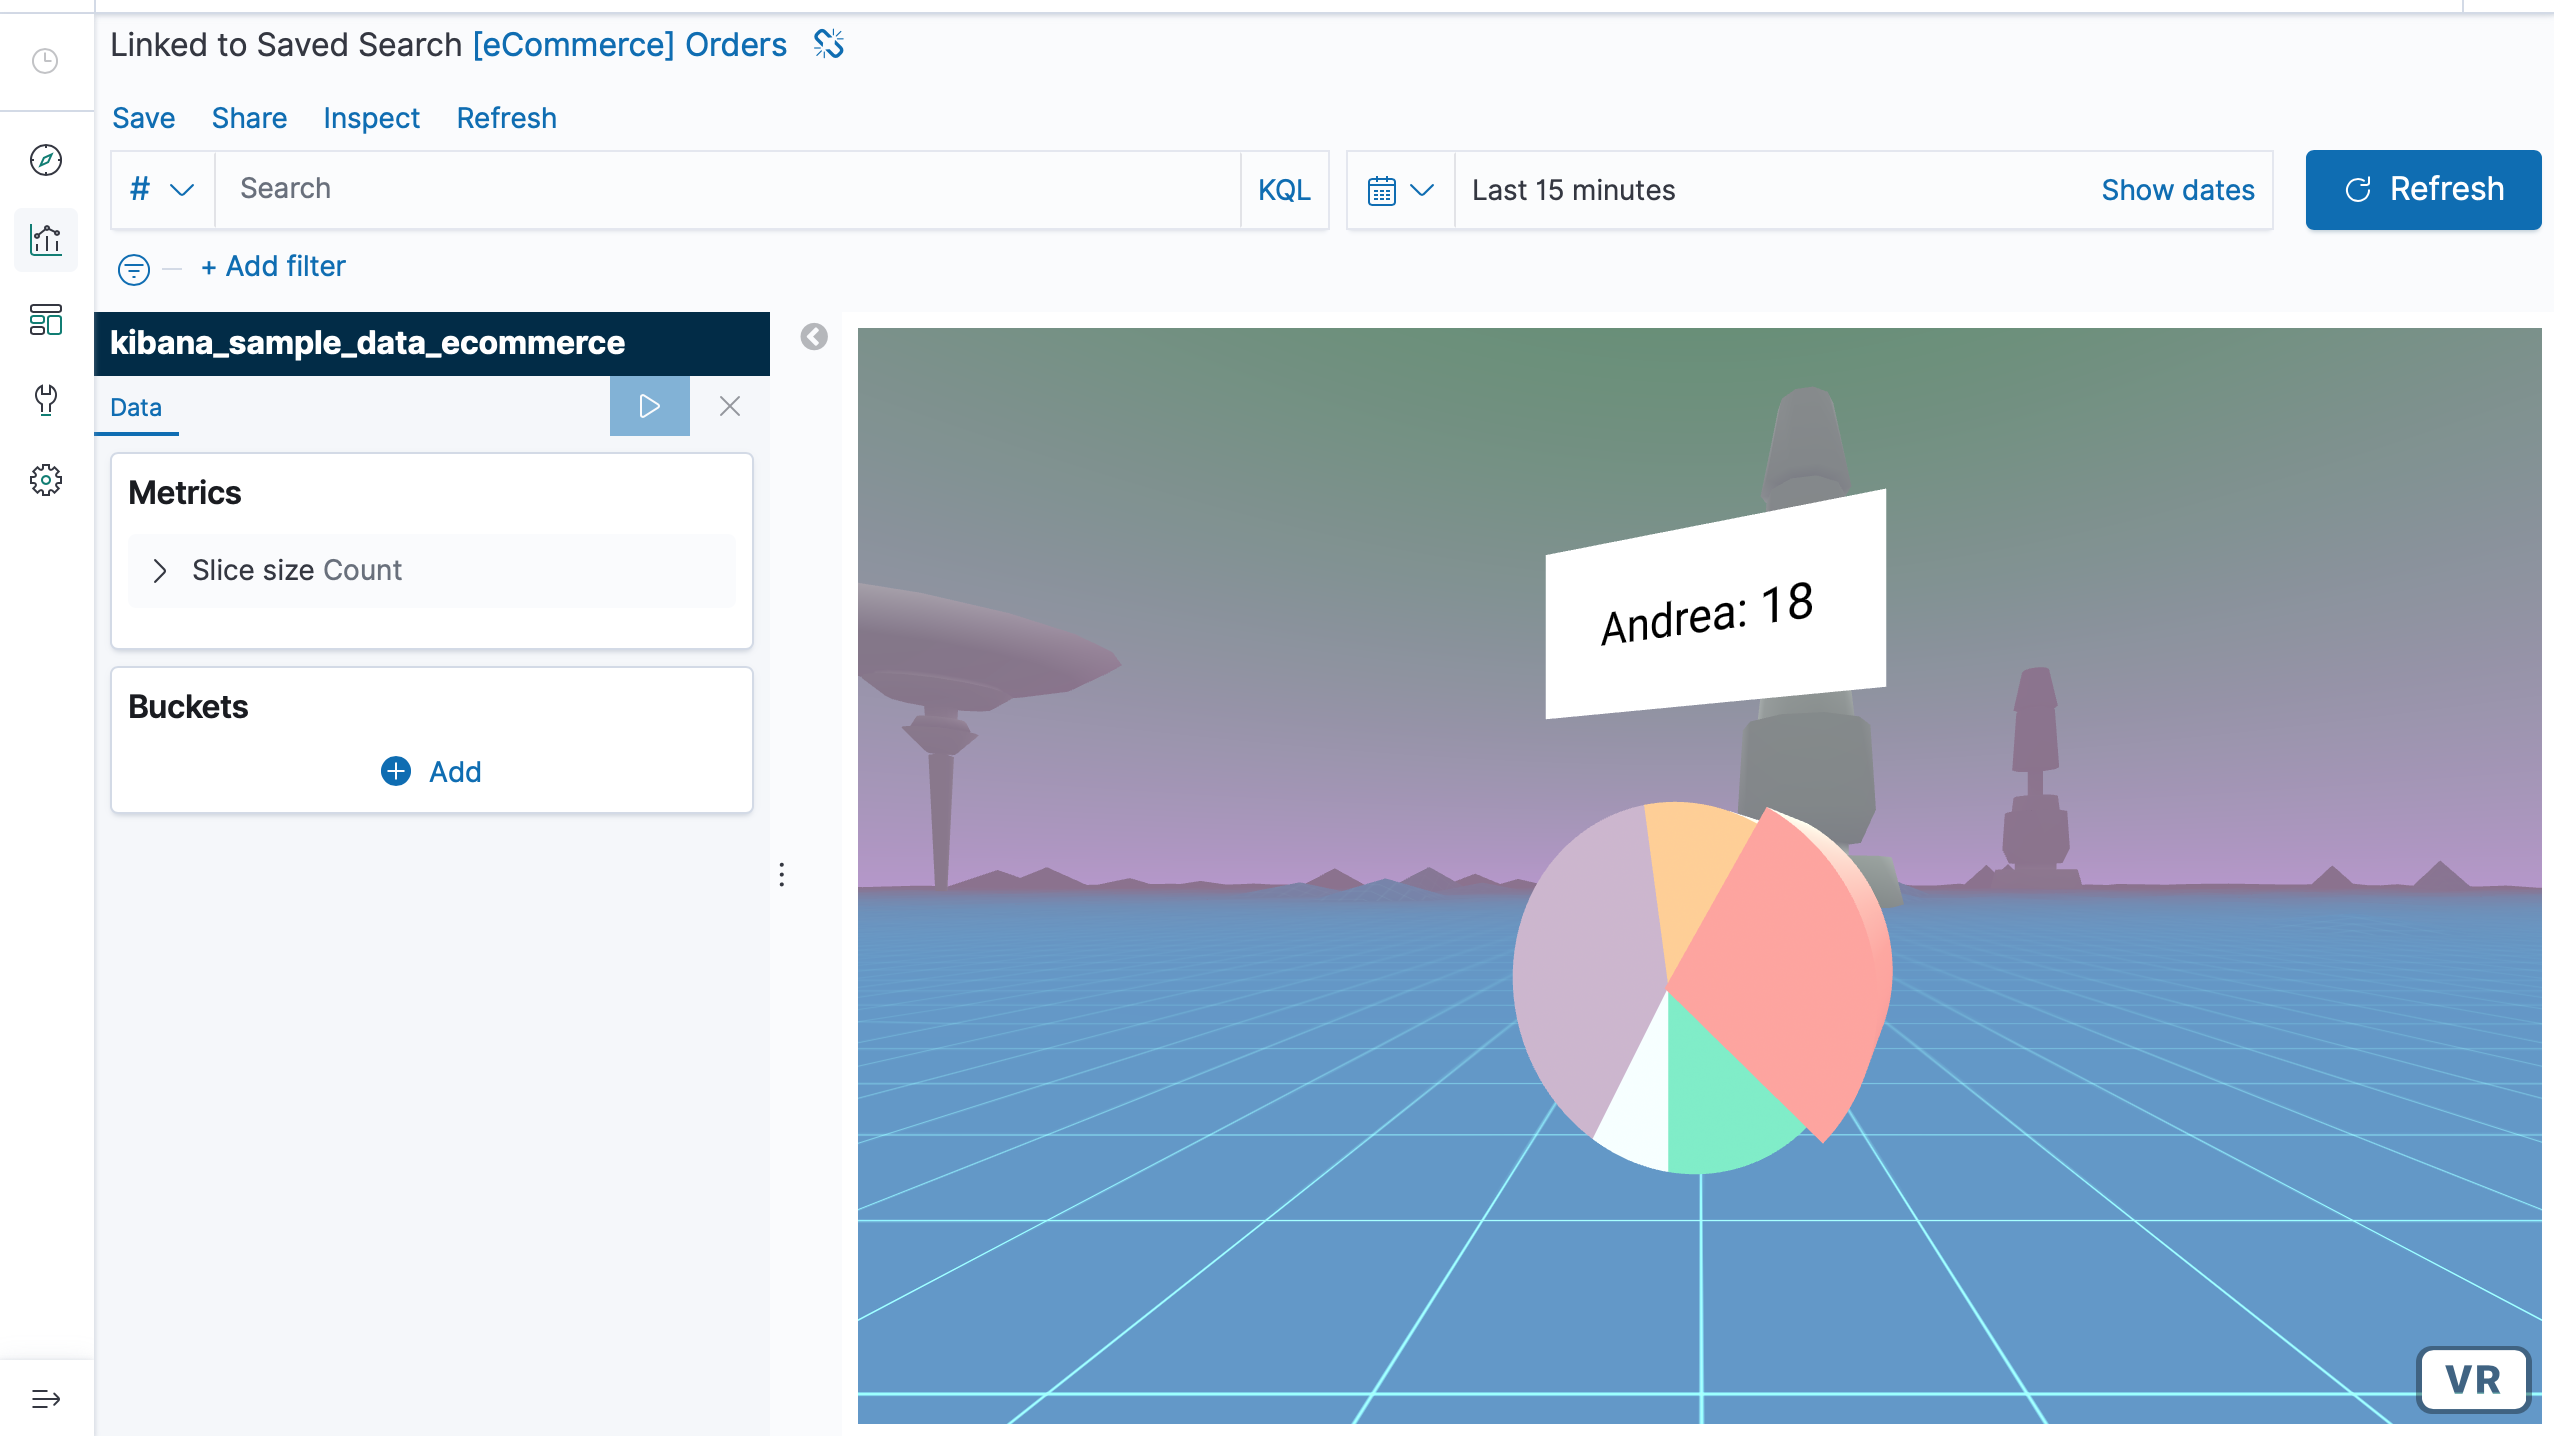
\includegraphics[width=12cm, keepaspectratio]{img/development/pie-sin-data.png}
  \caption{Resultado implementacion de geopiechart sin datos}
  \label{fig:piesindata}
\end{figure}



% PIE CHART CON DATOS
\subsection{Visualización Pie Chart con Datos}
\label{sec:piewithdata}

Ahora que ya sabemos que se puede implementar el componente de BabiaXR; lo último que nos queda para terminar este sprint es hacer que se cree el componente \textit{geopiechart} usando los datos que nos devuelve Kibana de Elasticsearch.

Lo primero será ver qué tipo de datos necesitaremos y lo indicaremos en el editor para que Kibana pueda hacer su correspondiente.

Como trabajamos con un formato de \textit{key-size}, utilizaremos un \textit{Bucket} que nos dará las keys y una \textit{Metric} que nos devolverá un valor por cada key. Una vez establecido esto, procedemos a configurar el editor, de la misma forma que lo hicimos en el Sprint 2 en \ref{sec:schemas}.

\lstinputlisting[language=Javascript]{code/iteracion3-kbn_aframe2.js}

Tal y como vimos también anteriormente cuando creamos el cubo a partir de datos en el capítulo  \ref{sec:aframecondatos}; tomaremos esa referencia para crear el \textit{data\_json} según el formato que nos indica BabiaXR. 

Esta vez es la primera vez que trabajamos con un bucket, por lo que la forma de sacar las métricas será diferente, ya que ahora debemos trabajar con las keys del \textit{bucket} y no solo con \textit{metrics}. Es decir, en esta ocasión, meteremos en metrics los valores obtenidos en forma de diccionario.

\lstinputlisting[language=Javascript]{code/iteracion3-kbn_aframe_controller6.js}

Ahora nos encontramos con la situación de que el componente \textit{geopiechart} necesita que le pasemos los datos en formato JSON, por lo que le damos ese formato usando la función \textit{JSON.stringify()}.

\lstinputlisting[language=Javascript]{code/iteracion3-kbn_aframe_controller7.js}

Con esto, hemos conseguido que a partir de ahora los datos que introducimos desde el editor sean mostrados en una gráfica tipo Pie.

\begin{figure}[H]
  \centering
  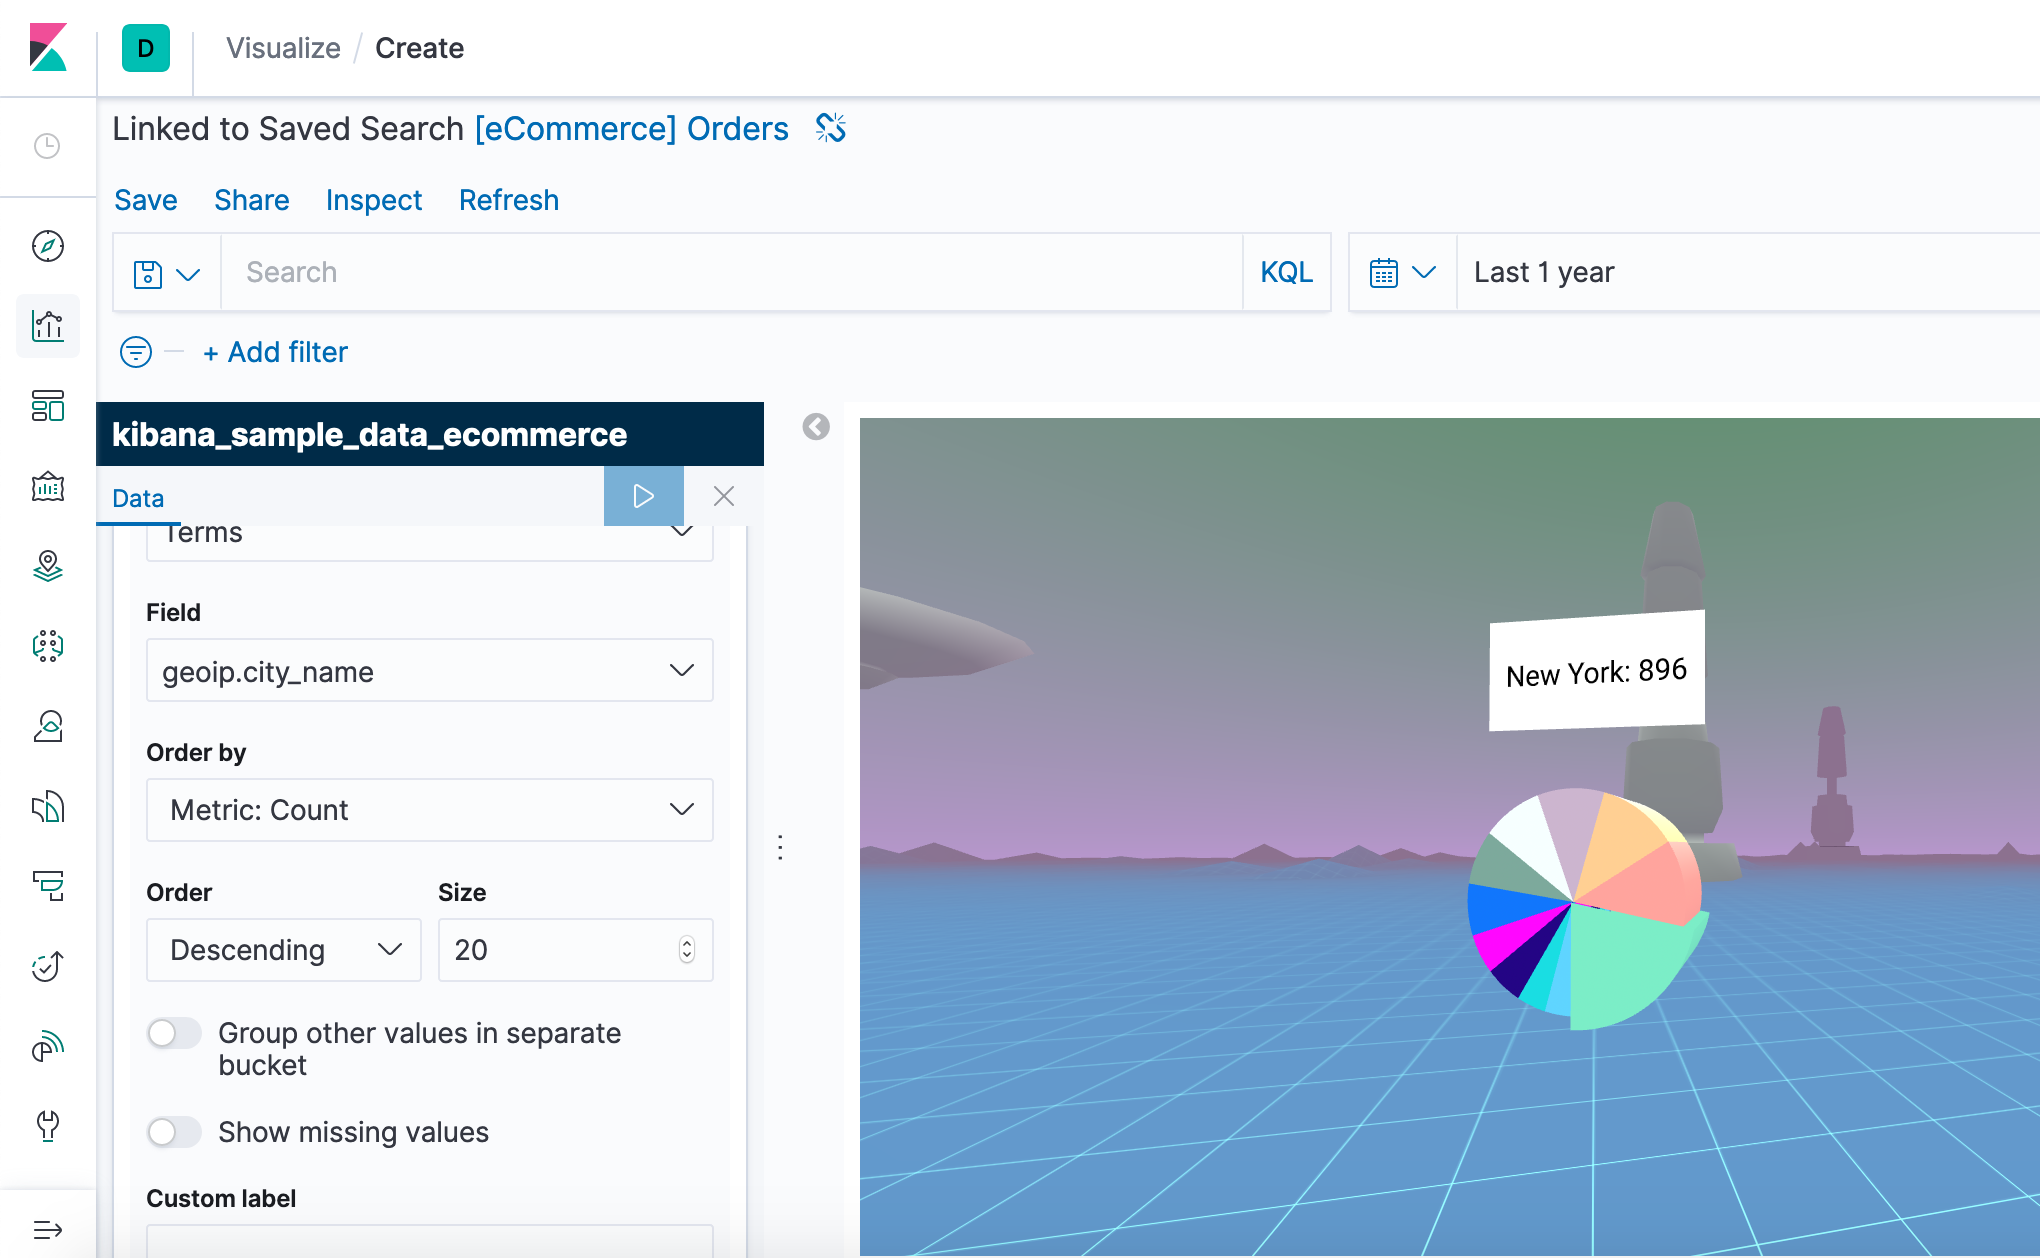
\includegraphics[width=12cm, keepaspectratio]{img/development/pie-con-data.png}
  \caption{Resultado de geopichart usando datos de Kibana}
  \label{fig:piecondata}
\end{figure}

Para obtener esta gráfica, le hemos pedido a Kibana que nos muestre el número de ventas segmentadas por ciudad; y que solo nos muestre las 20 con más ventas.

%%%%%%%%%%%
% SPRINT 4
%%%%%%%%%%%

\section{Sprint 4: Nuevas Visualizaciones }
\label{sec:sprint4}

En este último sprint, incluiremos el resto de componentes que existen actualmente dentro del módulo de BabiaXR. También aprovecharemos para optimizar el código y prepararlo en caso de querer añadir más características o más visualizaciones, como ocurrirá en este sprint.

Como cada componente utiliza diferentes tipos de formato a la hora de introducir los datos, iremos desde el más sencillo hasta el más complejo. Dicho esto, establecemos que las tareas de este sprint serán:

\begin{enumerate}
    \item Crear visualización con geosimplebarchart.
    \item Crear visualización con geo3dbarchart.
    \item Crear visualización con geobubblechart.
\end{enumerate}

\subsection{Visualización Simple Bar}
\label{sec:simplebar}

A primera vista parece que es muy sencillo de hacer, pero hay que tener un par de cosas en cuenta que antes no teníamos; pues esta es la primera vez que tenemos que registrar dos visualizaciones en un mismo plugin. Hasta ahora siempre habíamos trabajado con una sola visualización por plugin. 

En realidad esta parte es muy sencilla pues simplemente hay que crear otra constante con los parámetros de la visualización y registrarla. 

Analizando un poco cómo lo hacen los desarrolladores de Kibana, vemos que crean las definiciones de las visualizaciones en archivos individuales que luego importan en el fichero principal y únicamente hay que registrar las visualizaciones en él. 

Por eso, comenzaremos trasladando el código con la definición de la visualización de piechart a otro fichero que llamaremos \textit{pie.js}. 

Otro de los detalles a tener en cuenta es cómo el controlador va a saber que se trata de una gráficas u otras, ya que usaremos el mismo controlador para todas las visualizaciones que vamos a introducir. Para eso, existe un parámetros dentro de la definición de la visualización que permite pasar datos que luego recogeremos en \textit{this.vis.params} dentro del controlador.

Este parámetros es \textit{visConfig} y nos permite introducir datos por defecto desde la definición de la visualización o a través del editor en caso de crear una pestaña con opciones. 

Para nuestro caso, usaremos la opción por defecto y en ella le indicaremos que añada el tipo de gráfica de cada una de las visualizaciones. Esto hará que tengamos una variable que nos ayuda a identificar qué gráfica es y cómo proceder a la hora de coger las métricas y cómo construir la gráfica.

Así que, añadiremos esta líneas dentro de la definición de pie chart que ya se encuentra en \textit{pie.js}.

\lstinputlisting[language=Javascript]{code/iteracion4-pie1.js}

Al mismo tiempo, vamos a necesitar exportar la definición de la visualización de pie chart para poder importarla más adelante.

\lstinputlisting[language=Javascript]{code/iteracion4-pie2.js}

Una vez que ya tenemos trasladada la definición de pie chart, crearemos otra definición para la nueva visualización. Anteriormente se mencionó que iríamos desde la más sencilla a la más compleja. Para esto analizamos el formato de cada uno de los componente que hay en Kibana y los comparamos con el que ya tenemos implementado. A primera vista el componente \textit{geosimplebarchart} es el más parecido al \textit{geopiechart} pues su formato JSON son exactamente iguales.

Por tanto, procedemos a definir la nueva visualización en \textit{simple\_bar.js}:

\lstinputlisting[language=Javascript]{code/iteracion4-simple-bar1.js}

Como se ve, hemos añadido también el \textit{type} dentro de \textit{visConfig} para indicarle que esta visualización es en la que queremos crear una gráfica usando el componente \textit{geosimplebarchart}.

Lo que sigue es importar las definiciones, la que ya teníamos y la nueva, dentro del fichero \textit{kbn\_aframe.js}.

\lstinputlisting[language=Javascript]{code/iteracion4-kbn-aframe1.js}

Y registramos la nueva visualización:

\lstinputlisting[language=Javascript]{code/iteracion4-kbn-aframe2.js}

Desde Kibana ya se podrá ver que ya se puede crear un nuevo tipo de gráfica; pero antes haremos un par de modificaciones en la lógica de nuestro controlador; pues si lo dejamos tal cual dibujará también una gráfica tipo pie.

Para arreglar esto hemos creado el parámetro type en la definición de cada visualización. Esta se guarda dentro de la variable \textit{this.vis.params.type} y con ella trabajamos para que cree la gráfica de forma correcta para cada caso.

\lstinputlisting[language=Javascript]{code/iteracion4-kbn-aframe-controller1.js}

Hasta esta parte, la nueva visualización funciona sin problemas; pero decidimos anteriormente que íbamos a optimizar un poco el código para que fuera un poco más fácil de comprender en caso de que alguien quiere contribuir más adelante.

Como primera parte de esta tarea pasaremos las partes que siempre será igual en todos los escenarios a otras funciones que irán en módulos a parte y que los incluiremos en el render con sus llamadas correspondientes. Estas partes serán la de creación del entorno y la de insertar la camara y controles. Lo haremos de esta manera porque una parte tiene más que ver con el aspecto estético de la escena y el otro más con la parte del manejo y controles sobre la escena.

Empezamos trasladando el código en el que creamos la escena, el entorno y las luces a un función \textit{createScene()} que exportamos. Este fichero los nombramos \textit{a\_scene.js}.

\lstinputlisting[language=Javascript]{code/iteracion4-a-scene1.js}

Hacemos lo mismo con la líneas correspondientes a la creación de los controles y la cámara; y lo metemos en la función \textit{createControls()} dentro del nuevo fichero \textit{a\_controls.js}.

\lstinputlisting[language=Javascript]{code/iteracion4-a-controls1.js}

Hecho esto, importamos estas funciones en \textit{kbn\_aframe\_controller.js} y hacemos las llamadas correspondiente donde antes teníamos esa parte de código.

\lstinputlisting[language=Javascript]{code/iteracion4-kbn-aframe-controller2.js}

Finalmente podemos irnos a Kibana para ver los resultados.

\begin{figure}[H]
  \centering
  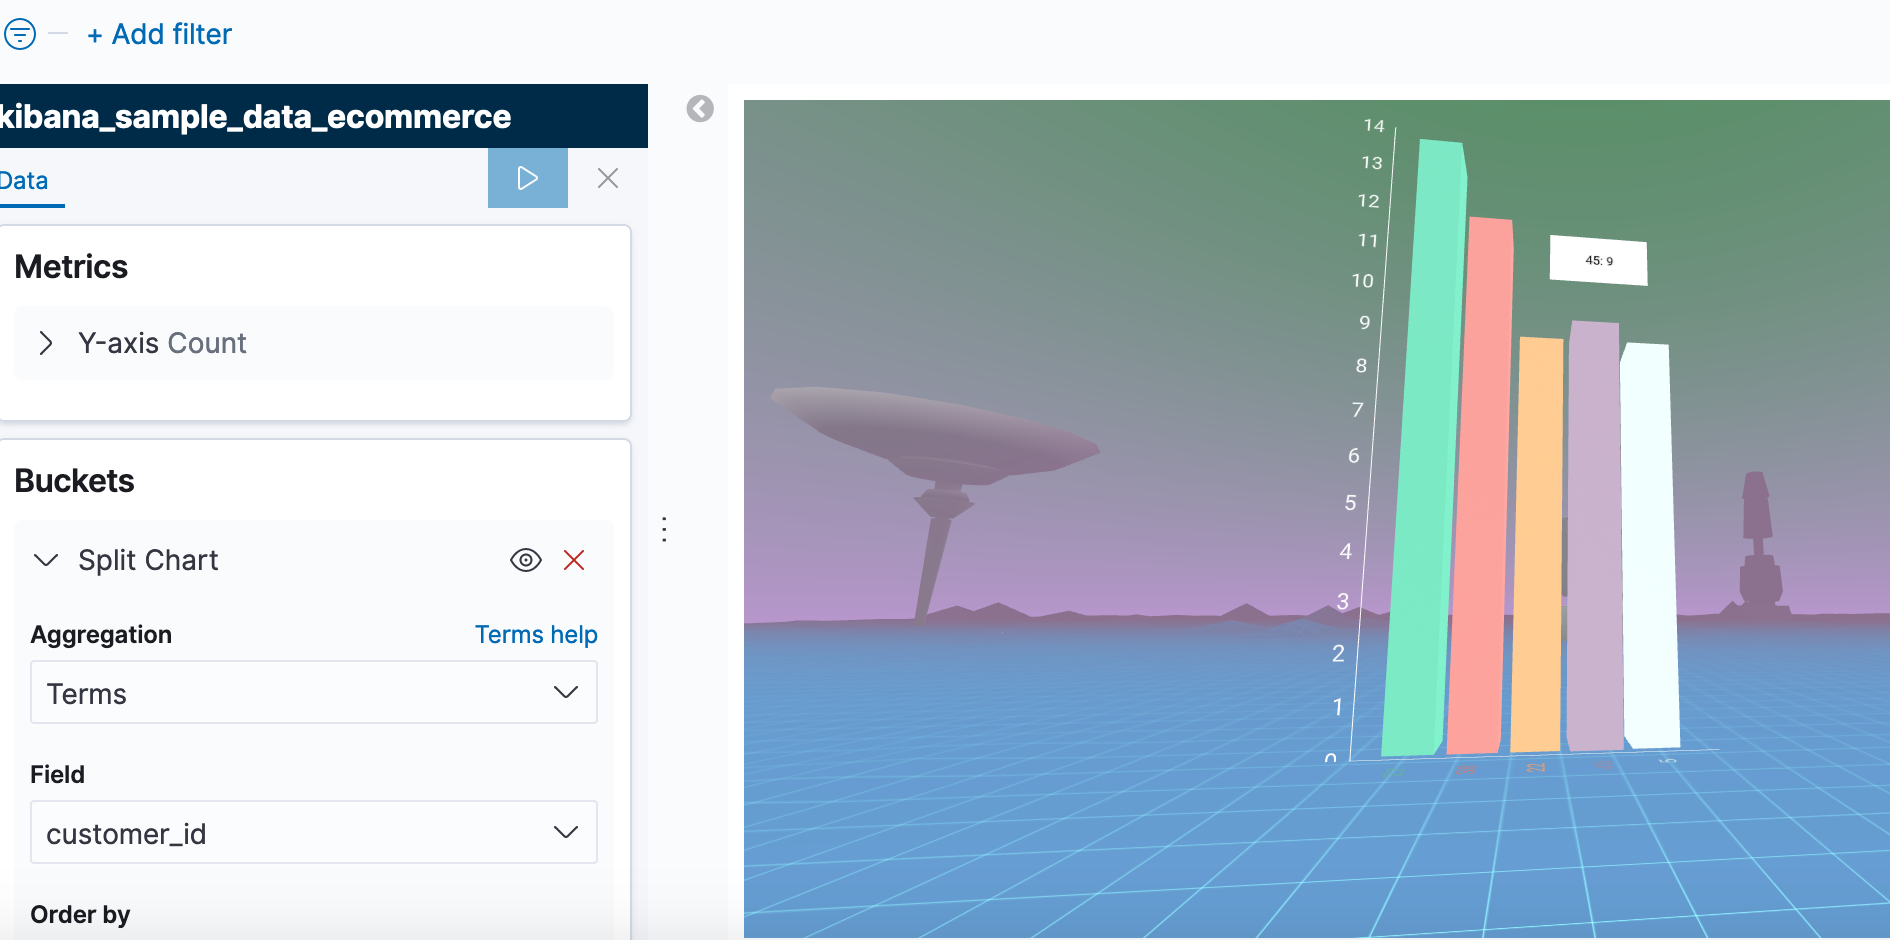
\includegraphics[width=12cm, keepaspectratio]{img/development/barchart.png}
  \caption{Resultado visualización Simple Bar Chart}
  \label{fig:simplebarchart}
\end{figure}

Para este ejemplo le hemos pedido que nos muestre lo usuarios que han hecho más compras durante un periodo de tiempo, se les etiqueta por id de usuario; y que nos muestre con la altura de la barra la cantidad de dichas compras.

\subsection{Visualización 3D Bars}
\label{sec:3dbars}

Seguimos incluyendo nuevas visualizaciones. En esta ocasión agregaremos una visualización que creará un gráfica de barras en 3D usando el componente \textit{geo3dbarchart}. A partir de aquí, los componentes que añadamos no tendrán el mismo formato JSON como tenian \textit{geopiechart} y \textit{geosimplebarchart} \footnote{\url{https://github.com/babiaxr/aframe-babia-components#data-format-2}}.

\lstinputlisting[language=JSON]{code/iteracion4-geo3dbarchart.json}

Analizando el formato JSON de \textit{geo3dbarchart}, vemos que en esta ocasión existe una nueva variable que es \textit{key2}. Esta indica que, al igual que \textit{key}, corresponde a una forma de etiquetar cada valor mostrado, en este caso serán dos etiquetas por valor. Esto. en términos visuales, lo que hará es etiquetar las barras en los ejes X y Z. 

Una vez hemos comprendido esto, ya podemos determinar como será nuestro editor. Trabajaremos con 2 claves y un valor, lo que en término del editor de Kibana se traduce en 2 buckets y un metric. 

Determinado esto, procedemos a crear la definición de la nueva visualización en \textit{3dbar.js}.

\lstinputlisting[language=Javascript]{code/iteracion4-3dbar.js}

Como se ve en la configuración del editor, le estamos indicando que debe tener 2 buckets porque sino la gráfica no se dibujará.

Y procedemos a registrarla dentro en \textit{kbn\_aframe}.

\lstinputlisting[language=Javascript]{code/iteracion4-kbn-aframe3.js}

Ahora que hemos registrado la visualización, pasamos a la parte del controlador. Empezando por la parte de la obtención de los datos que luego pasamos a JSON para luego crear su correspondiente gráfica. A cada caso que metemos, el código se vuelve más grande, por lo que se tomó la decisión de sacar de \textit{render()} y crear una función \textit{getMetrics()} para solo centrarnos en esa parte. 

Esta función se encontrará en un fichero \textit{metrics.js}, donde le introduciremos los datos y el tipo de visualización para que nos devuelva sus correspondientes datos, perfectamente estructurados según el formato de cada tipo, para posteriormente convertirlos en JSON.

\lstinputlisting[language=Javascript]{code/iteracion4-metrics1.js}

Una vez hemos trasladado el código con sus correspondientes modificaciones para el caso de la nueva visualización, procedemos a importar la función y llamarla donde antes teníamos las líneas para obtener las métricas.

\lstinputlisting[language=Javascript]{code/iteracion4-kbn-aframe-controller4.js}

Por último nos faltaría añadir el caso del nuevo componente en la parte donde creamos las gráficas; pero ,al igual que con la obtención de métricas, nos encontramos que a cada caso nuevo que añadimos, el código se vuelve más complejo. Por lo que los sacaremos también y lo metemos en una nueva función \textit{createChart()} dentro de un nuevo fichero \textit{a\_charts.js}.

A esta función se le pasar los datos, ya en JSON, y el tipo de visualización en la que estamos; y nos devolverá la entidad que contiene la gráfica correspondiente para luego añadirla a la escena.

A esto, le añadimos también las nuevas líneas con el caso para crear una gráfica con el componente \textit{geo3dbarchart}.

\lstinputlisting[language=Javascript]{code/iteracion4-a-charts1.js}

Y por último, importamos al función al controlador y hacemos la llamada donde corresponde.

\lstinputlisting[language=Javascript]{code/iteracion4-kbn-aframe-controller5.js}

Con esto obtenemos la siguiente visualización en Kibana.

\begin{figure}[H]
  \centering
  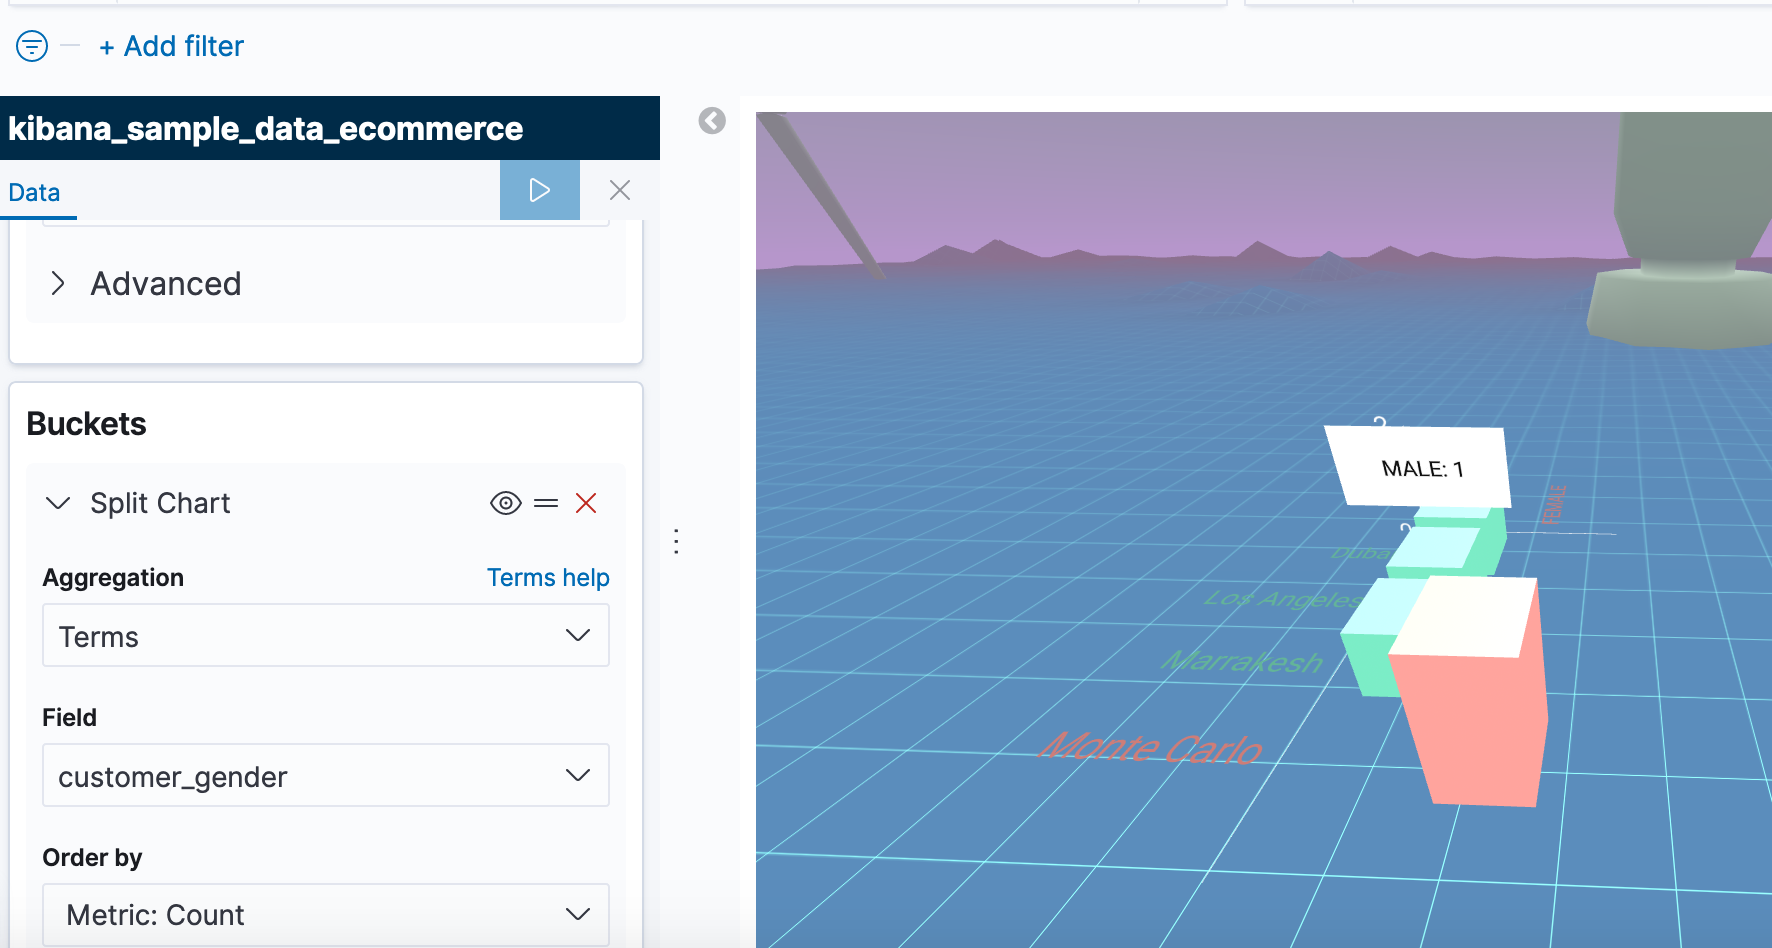
\includegraphics[width=12cm, keepaspectratio]{img/development/3d-bar-chart.png}
  \caption{Resultado Visualización 3D Bars Chart.}
  \label{fig:3dbarchart}
\end{figure}

Para este ejemplo, le hemos pedido que nos muestre las ventas que se han realizado en función del género de comprador y la ciudad donde se ha realizado la compra.

\subsection{Visualización Bubbles}
\label{sec:bubbles}

Por último, sólo nos queda crear la visualización de tipo bubbles. A partir de aquí será más sencillo pues al haber reestructurado el código, según van apareciendo nuevos casos, únicamente habrá que añadir las líneas correspondientes a dicho caso.

Al igual que hemos hecho anteriormente con el resto de visualizaciones, empezaremos determinando cómo vamos a tratar los datos.

Según la documentación de BabiaXR para el componente \textit{geobubblechart}, el formato de nuestro JSON deberá ser el siguiente\footnote{\url{https://github.com/babiaxr/aframe-babia-components#data-format-3}}:

\lstinputlisting[language=JSON]{code/iteracion4-geobubbleschart.json}

Como vemos, en esta ocasión vamos a trabajar con dos claves: \textit{key} y \textit{key2}; con dos valores: \textit{height} y \textit{radius}. Esto, en términos del editor de Kibana, lo traducimos en dos buckets y dos metrics. Una vez determinado esto, procedemos a crear la definición de esta nueva visualización en \textit{bubble.js}.

\lstinputlisting[language=Javascript]{code/iteracion4-bubble.js}

Y, al igual que hicimos con las anteriores visualizaciones, lo importamos a \textit{kbn\_aframe.js} y registramos la visualización.

\lstinputlisting[language=Javascript]{code/iteracion4-kbn-aframe4.js}

Nos vamos a la parte del controlador; pero en esta ocasión directamente editaremos sobre las funciones de \textit{getMetrics()} y \textit{createChart()} que se encuentran en \textit{metrics.js} y \textit{a\_charts.js} correspondientemente.

Siguiendo los pasos que seguimos con las otras visualización, añadimos las nuevas líneas correspondientes para estructurar los datos obtenidos de Elasticsearch al formato que necesitamos para poder crear el componente en la función \textit{getMetrics()}.

\lstinputlisting[language=Javascript]{code/iteracion4-metrics2.js}

Y por último, añadir el caso de esta nueva visualización y que nos cree el componente \textit{geobubblechart}.

Obteniendo en Kibana una visualización resultado con una gráfica de tipo bubble.

\begin{figure}[H]
  \centering
  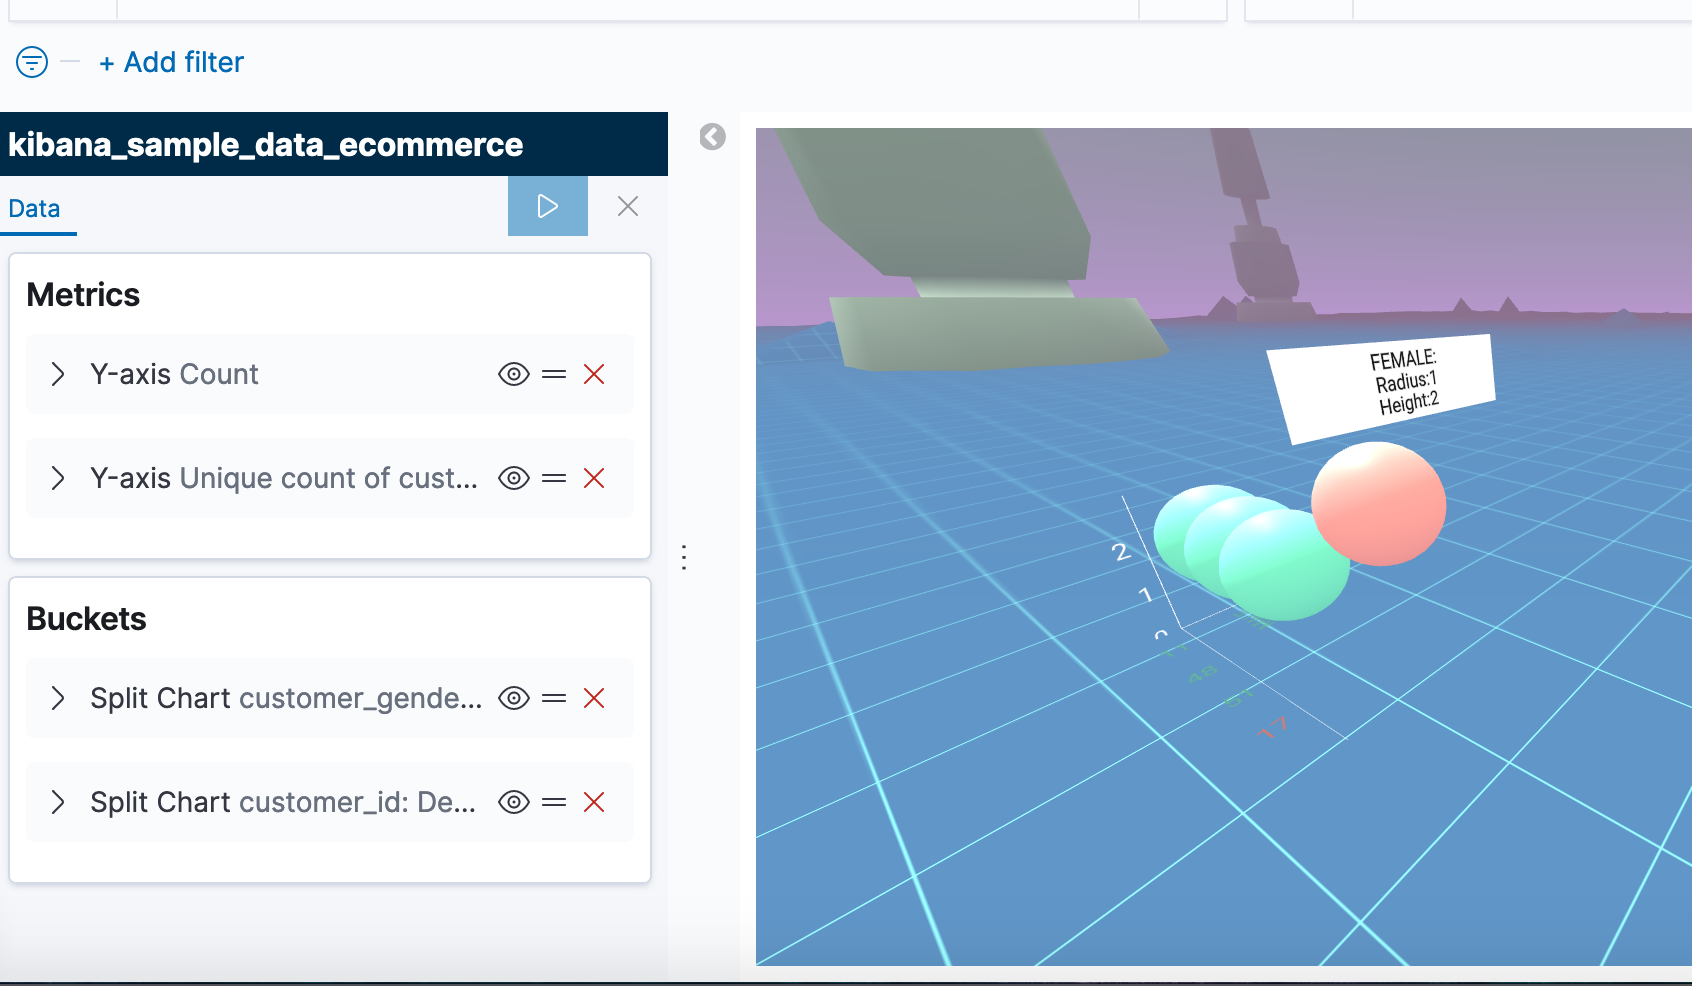
\includegraphics[width=12cm, keepaspectratio]{img/development/bubbles-chart.png}
  \caption{Resultado Visualización Bubble Chart}
  \label{fig:bubblechart}
\end{figure}

Para este ejemplo hemos tomado el número de ventas para determinar la altura, el contador uno por cada comprador y que nos los clasifique por id de usuario y según sexo.

Y tras haber añadido el último de los componente que hay actualmente en BabiaXR, damos por finalizado este sprint y con ello, finalizamos la parte de desarrollo de este proyecto.



%%%%%%%%%%%%%%%%%%%%%%%%%%%%%%%%%%%%%%%%%%%%%%%%%%%%%%%%%%%%%%%%%
% DISEÑO Y RESULTADOS %
%%%%%%%%%%%%%%%%%%%%%%%%%%%%%%%%%%%%%%%%%%%%%%%%%%%%%%%%%%%%%%%%%

\cleardoublepage
\chapter{Diseño y Resultados}
\label{sec:resultados} 

En este capítulo describiremos los resultados obtenidos al final del proyecto. Primero definiremos la arquitectura resultante del proyecto; y terminaremos con una guia de usuario donde explicaremos su uso mediante un caso hipotético. 

Para no repetir, se ha omitido el resultado de cada una de las visualizaciones (tal y como se mostró a lo largo de las últimas iteraciones del capítulo \ref{sec:desarrollo} ); y únicamente se explica cómo se crean en la guia de usuario. 

\section{Arquitectura General}
\label{sec:arquitectura}

Como explicamos anteriormente en el capítulo \ref{sec:entorno} para el desarrollo de un plugin en Kibana se debe tener una estructura mínima para poder funcionar. Partiendo de ella, añadimos otros ficheros que complementan el registro de visualizaciones y el controlador de éstas. Todo esto debe estar contenidos dentro del directorio del plugin que se encuentra dentro de la carpeta \textit{plugins/} del directorio principal de Kibana. 

A continuación se muestra la estructura final del proyecto:

\begin{figure}[H]
  \centering
  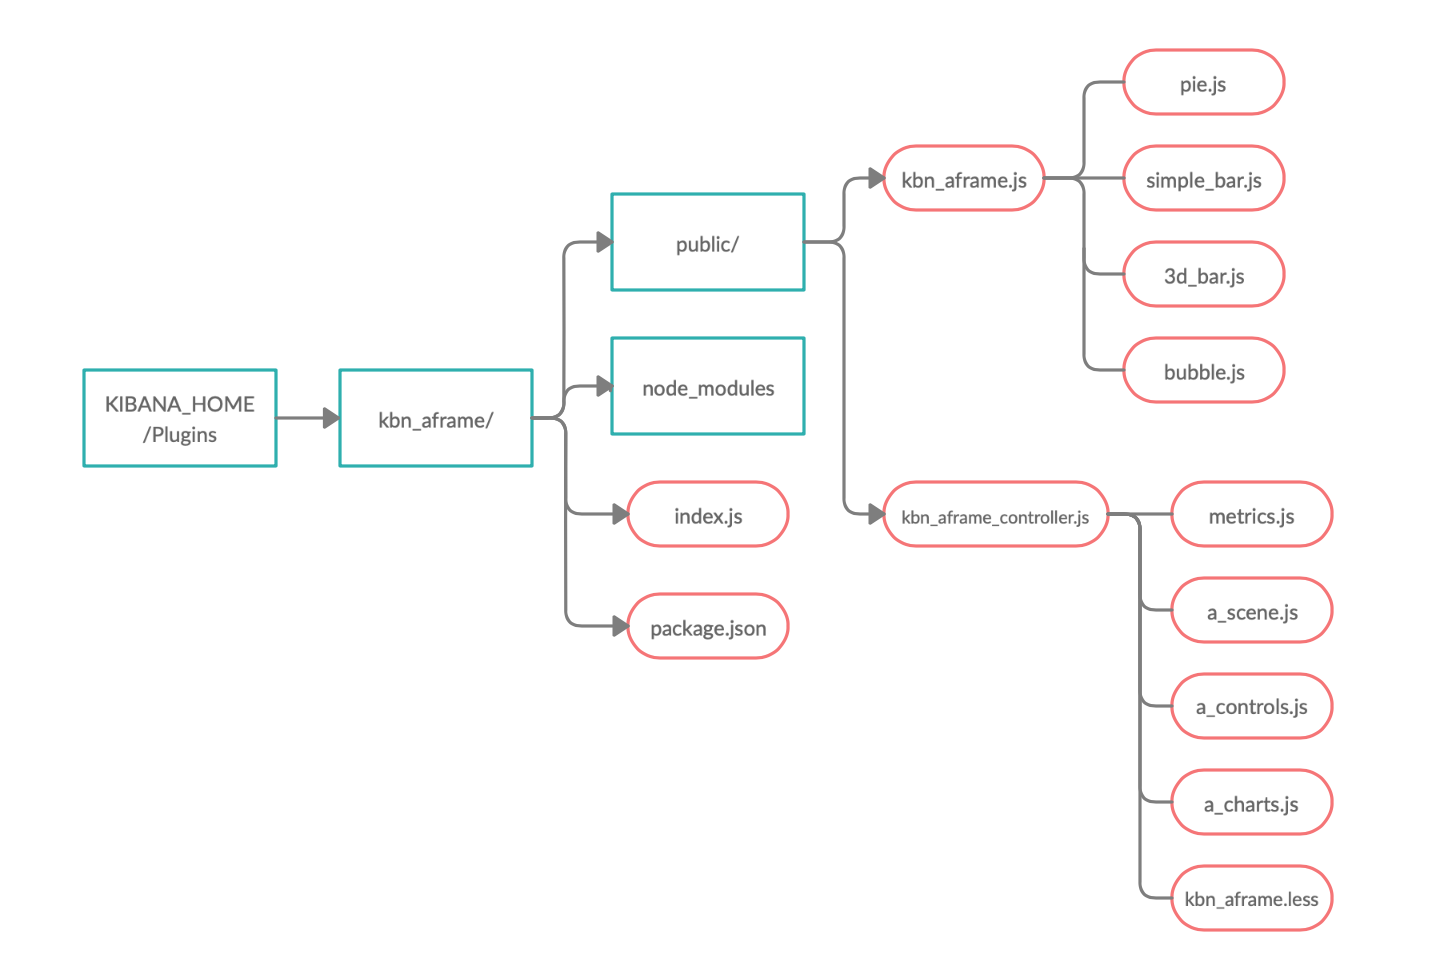
\includegraphics[width=12cm, keepaspectratio]{img/development/estructura-final.png}
  \caption{Estructura final del proyecto}
  \label{fig:arquitecturaproyecto}
\end{figure}

El contenido de cada fichero se muestra detalladamente en el repositorio del proyecto\footnote{\url{https://github.com/Camichan/kbn_aframe}}.

Descripción de los ficheros dentro del directorio del plugin:

\begin{itemize}
    \item \underline{package.json}: contiene los metadatos del plugin y las dependencias que se necesitaban instalar.
    \item \underline{index.js}: fichero javascript que define el plugin e indica dónde se encuentra el fichero principal del plugin.
    \item \underline{node\_modules/}: directorio donde se encuentran todos los módulos instalados.
    \item \underline{public/}: directorio donde se encuentra el contenido del plugin.
\end{itemize}

Dentro de este directorio nos encontramos con los siguientes ficheros:

\begin{itemize}
    \item \underline{kbn\_aframe.js}: es el fichero principal donde registramos cada una de las visualizaciones del plugin.
    \item \underline{pie.js}: contiene la definición de la visualización VR Pie.
    \item \underline{simple\_bar.js}: contiene la definición de la visualización VR Vertical Bar.
    \item \underline{3d\_bar.js}: contiene la definición de la visualización VR 3D Bar.
    \item \underline{bubble.js}: contiene la definición de la visualización VR Bubbles.
    \item \underline{kbn\_controller.js}: es el fichero que contiene el controlador de las visualizaciones.
    \item \underline{metrics.js}: contiene la parte que coge los datos y les da el formato que necesita cada una de las visualizaciones.
    \item \underline{a\_scene.js}: es la parte que crear el escenario A-Frame y le añade las luces.
    \item \underline{a\_controls.js}: esta parte añade la cámara y los controles al escenario de A-Frame.
    \item \underline{a\_charts.js}: esta parte se encarga de crear la gráfica a partir de los datos recibidos, en función de la visualización elegida.
    \item \underline{aframe.less}: contiene el estilo que le damos a la visualización.
\end{itemize}

Con esta arquitectura conseguimos que Kibana se encargue de proveer el marco de la visualización y de crear el editor en función de lo que le hayamos definido; y el plugin se encarga de representar los datos obtenidos mediante dicho editor.


\section{Guia de Usuario}
\label{sec:guiausuario}

Para una mejor comprensión del uso del plugin, expondremos un caso hipotético utilizando una de las bases de datos de prueba que nos proporciona Kibana. En esta ocasión, usaremos la de eCommerce. 

Imaginemos que tenemos un negocio de venta de ropa para hombre y mujer; y nos interesa conocer ciertos datos con referencia a nuestros clientes. Por ejemplo, desde donde nos compran, el sexo del cliente, etc. Antes de pasar a crear las visualizaciones para luego introducirlos en una Dashboard, debemos definir que clase de datos queremos que nos representen cada una de las visualizaciones:

\begin{itemize}
    \item Queremos saber el sexo de nuestro clientes para saber si debemos enfocar nuestros productos a mujeres, a hombre; o seguir como hasta ahora.
    \item Tenemos varias tiendas en distintas ubicaciones del mundo y queremos conocer cuales son las que reciben más ventas en caso de que queramos ampliar el dichas ciudades.
    \item En vista de que algunas de nuestras tiendas no están consiguiendo los beneficios que esperábamos se ha decidido prescindir, en dichas tiendas, de los artículos enfocados al sexo con menos ventas. Por lo que queremos conocer el volumen de ventas por género en dichas tiendas.
    \item Hacer una comparativa entre las ciudades con más ventas y la media de ventas en cada continente.
\end{itemize}

Una vez hemos decidido que visualizaciones vamos a crear, pasaremos a crearlas. Lo primero es ir a la pestaña de visualizaciones dentro de Kibana. Una vez ahí, le damos a \textit{Create New Visualization}.

A continuación vemos como nos aparecen las visualizaciones correspondientes a nuestro plugin:

\begin{figure}[H]
  \centering
  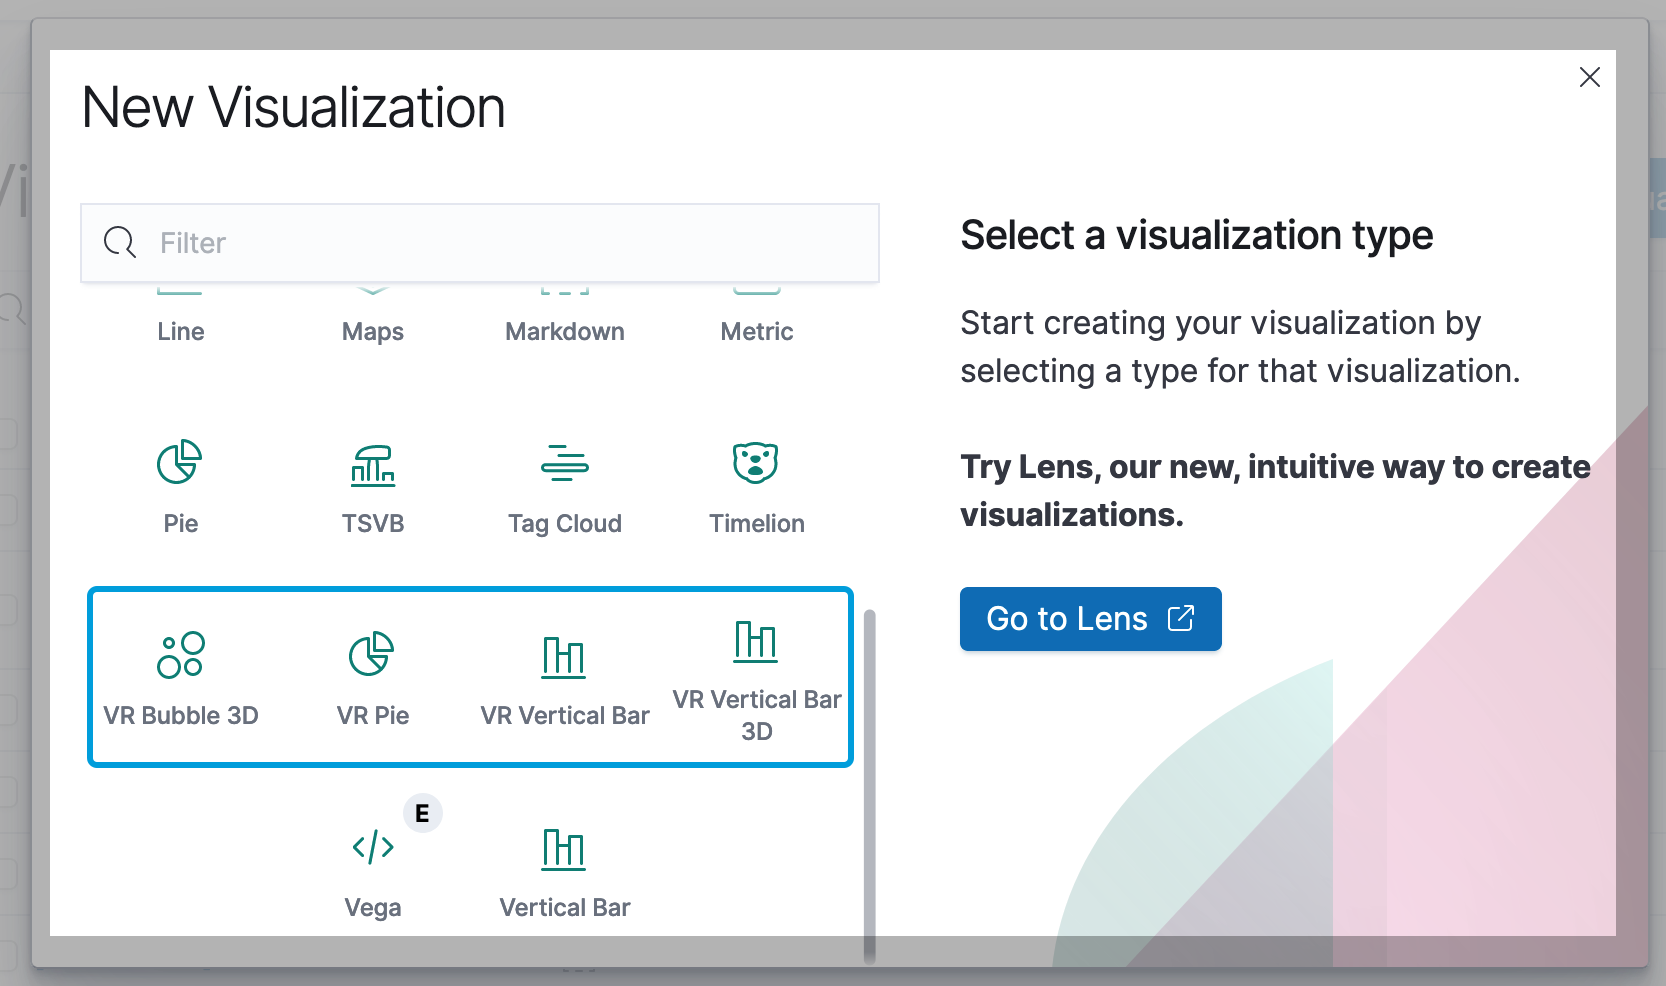
\includegraphics[width=10cm, keepaspectratio]{img/development/visualizaciones-menu-use.png}
  \caption{Menú con las visualizaciones del plugin}
  \label{fig:menuvisualizacionesuse}
\end{figure}

Comenzaremos con la visualización VR Pie. Seleccionamos nuestra base de datos y entramos dentro de la interfaz de la visualización. Aquí presentamos varios elementos.

\begin{figure}[H]
  \centering
  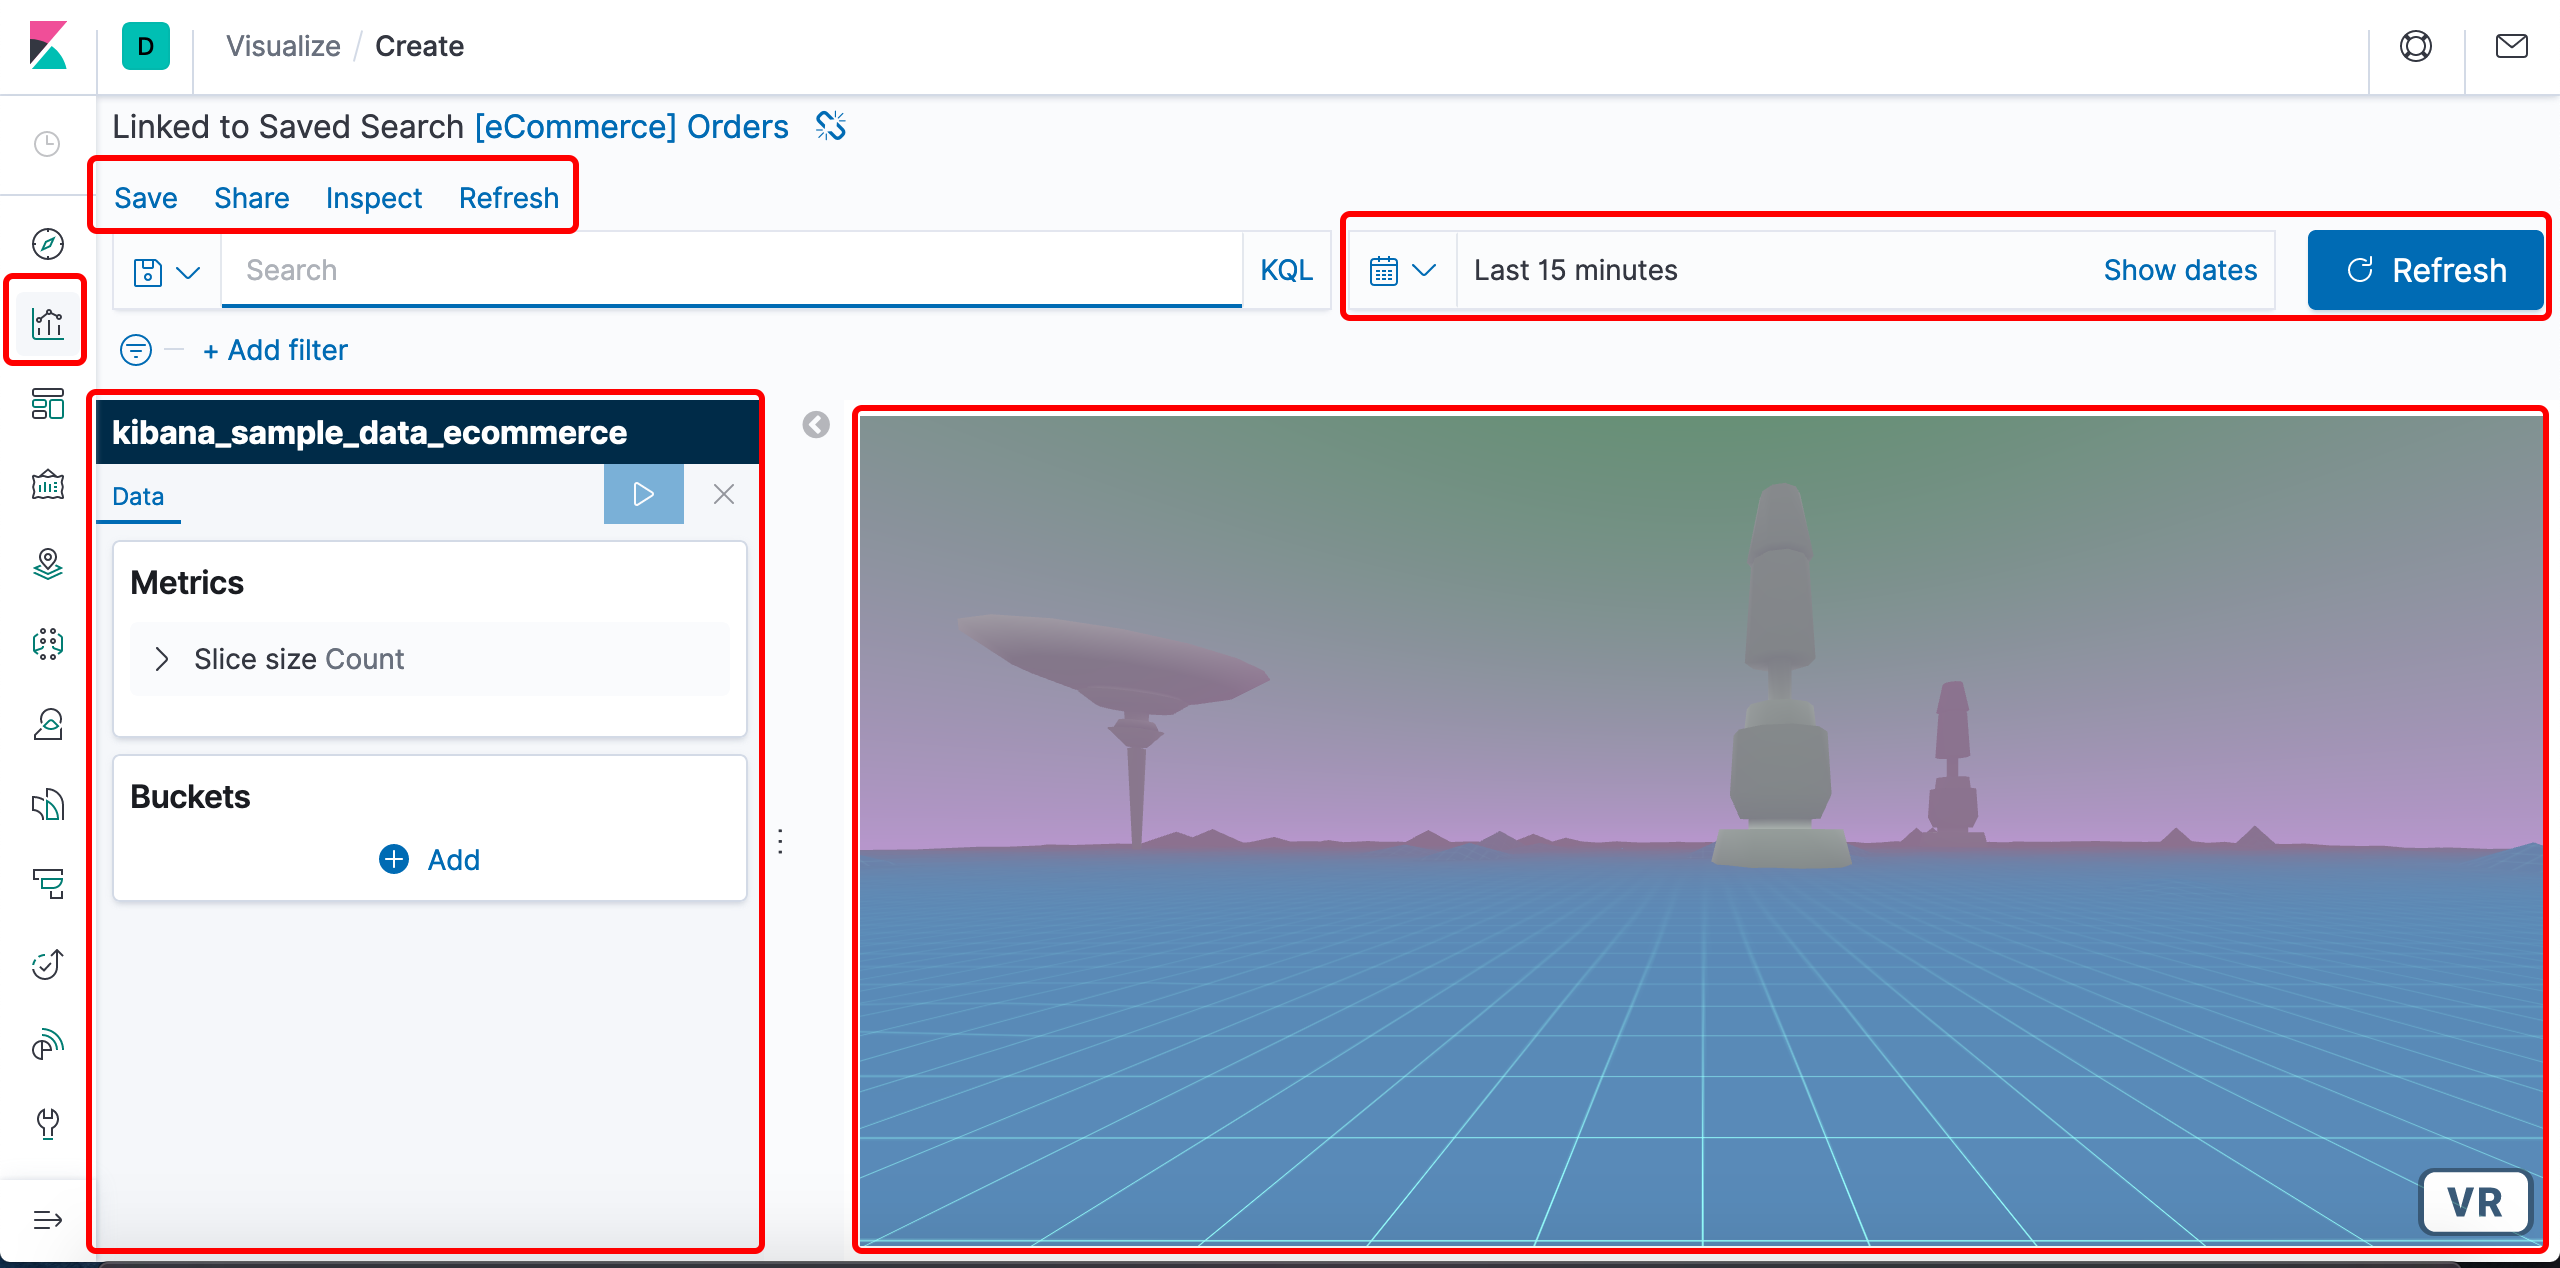
\includegraphics[width=14cm, keepaspectratio]{img/development/interfaz-visualizacion.png}
  \caption{Interfaz de visualización}
  \label{fig:interfazvisualizacion}
\end{figure}

A la izquierda tenemos el editor donde le introduciremos los datos que queremos que nos representen.

Arriba a la derecho tenemos un campo donde debemos introducir el rango de tiempo en el que se comprenden los datos que queremos que nos muestre.

En la esquina superior izquierda tenemos las opciones de guardado, compartir, inspeccionar y refrescar la visualización.

Y por último, en la esquina inferior derecha tenemos la visualización.

Para introducir los datos deberemos ir al editor y hacer la petición correspondiente. Para esta ocasión nos interesa conocer el sexo de nuestro clientes en los últimos meses, así que dejaremos la metric \textit{Count} que nos mostrará el número de ventas; y añadiremos un bucket con los siguientes parámetros.

\begin{figure}[H]
  \centering
  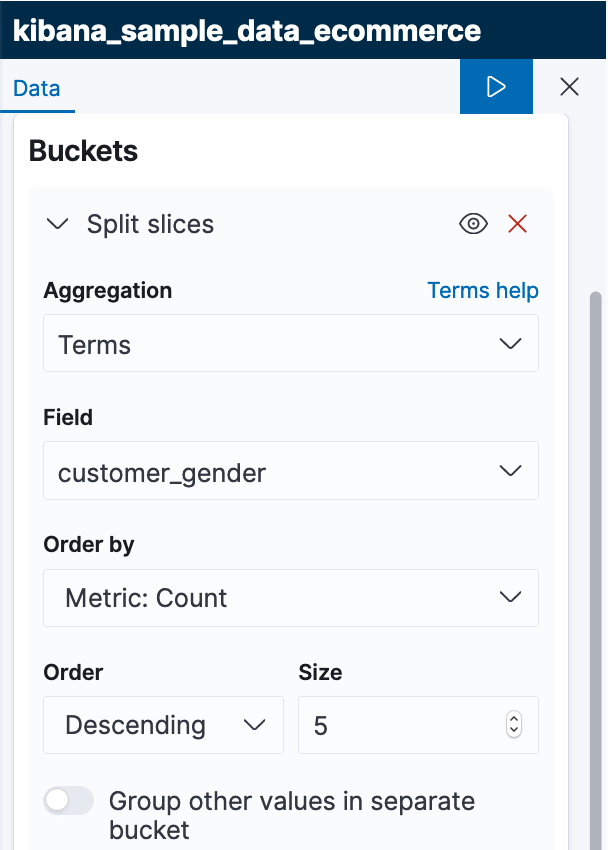
\includegraphics[width=5cm, keepaspectratio]{img/development/editor-pie.png}
  \caption{Editor de la visualización VR Pie}
  \label{fig:editorpie}
\end{figure}

Una vez introducidos, le damos en el botón de la esquina superior derecha del editor para actualizar la visualización. Obteniendo el siguiente resultado:

\begin{figure}[H]
  \centering
  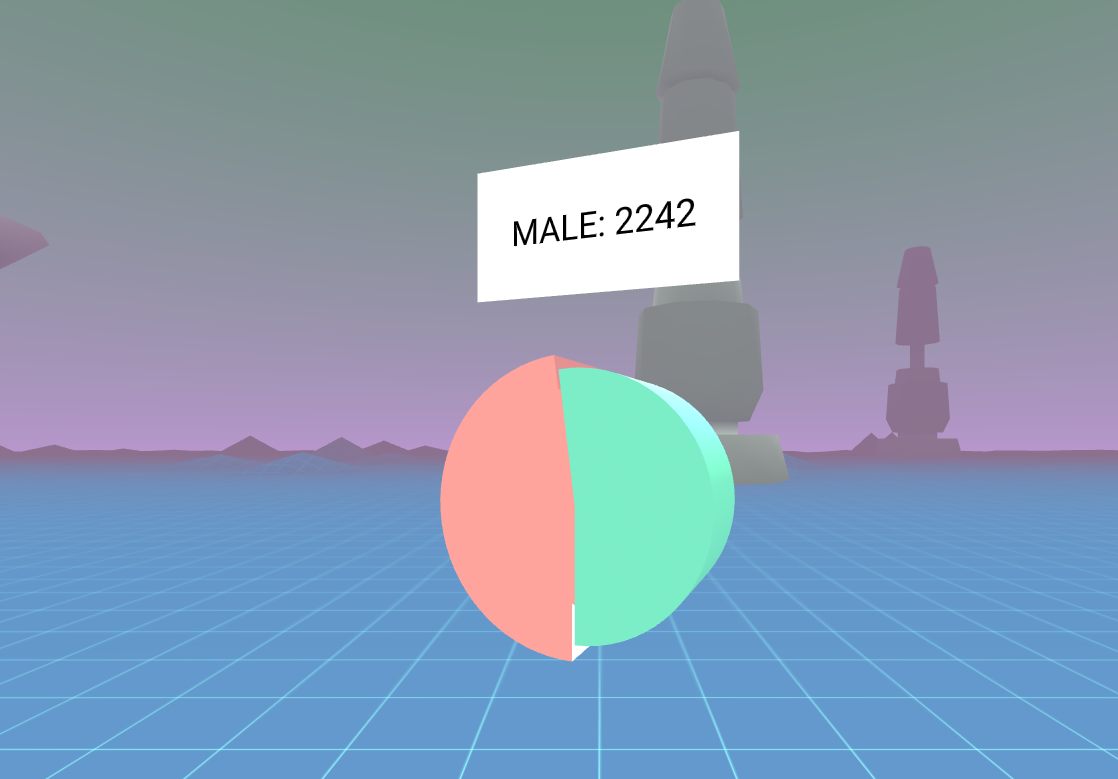
\includegraphics[width=10cm, keepaspectratio]{img/development/visualizacion-pie-use.png}
  \caption{Resultado de Visualización VR Pie}
  \label{fig:}
\end{figure}

Lo que lo diferencia de las otras visualizaciones es que nos podemos mover por el espacio usando las teclas de movimiento y el ratón. Incluso, en caso de poseer algún dispositivo de Realidad Virtual, poder interactuar dentro del escenario.

Cuando estemos satisfechos con la visualización, únicamente le damos a guardar y le añadimos un nombre y una descripción a la visualización, si así lo requiere.

\begin{figure}[H]
  \centering
  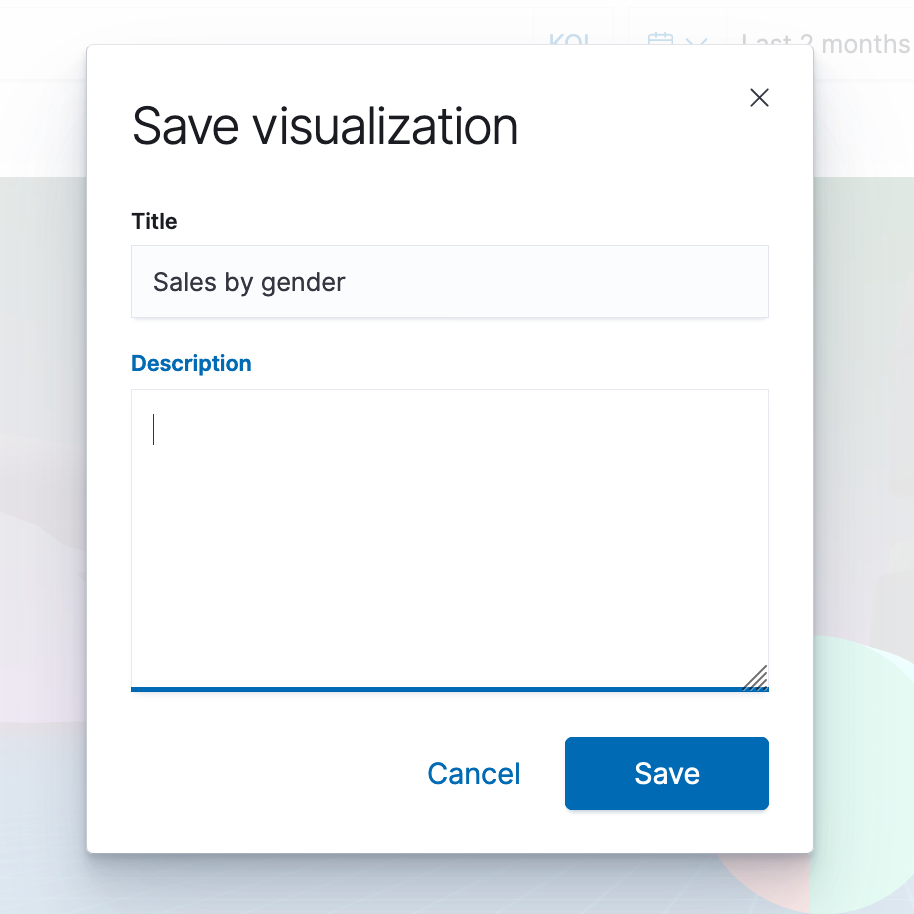
\includegraphics[width=6cm, keepaspectratio]{img/development/save.png}
  \caption{Interfaz de guardado.}
  \label{fig:guardado}
\end{figure}

A continuación pasamos a hacer lo mismo con las visualización de barras verticales. En este caso queremos conocer cuales son la localidades con más ventas en los últimos meses.

Hacemos exactamente lo mismo que hicimos anteriormente, pero esta vez seleccionando \textit{VR Vertical Bar}; y procedemos a seleccionar la petición en el editor.

\begin{figure}[H]
  \centering
  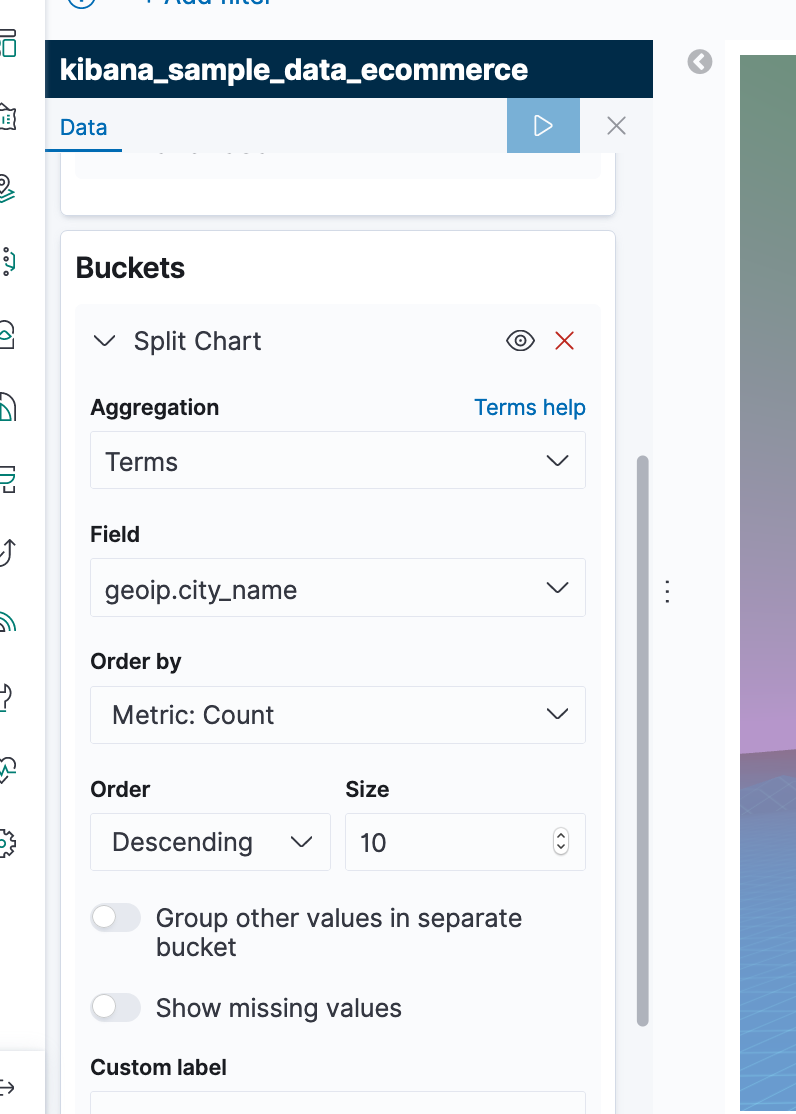
\includegraphics[width=5cm, keepaspectratio]{img/development/editor-bars.png}
  \caption{Editor para VR Vertical Bars}
  \label{fig:editorbars}
\end{figure}

La única diferencia con la anterior visualización es que, en esta ocasión, como nos interesa saber las 10 ciudades con más ventas, debemos indicarlo en los parámetros de \textit{order} y \textit{size}.

Obteniendo la siguiente visualización.

\begin{figure}[H]
  \centering
  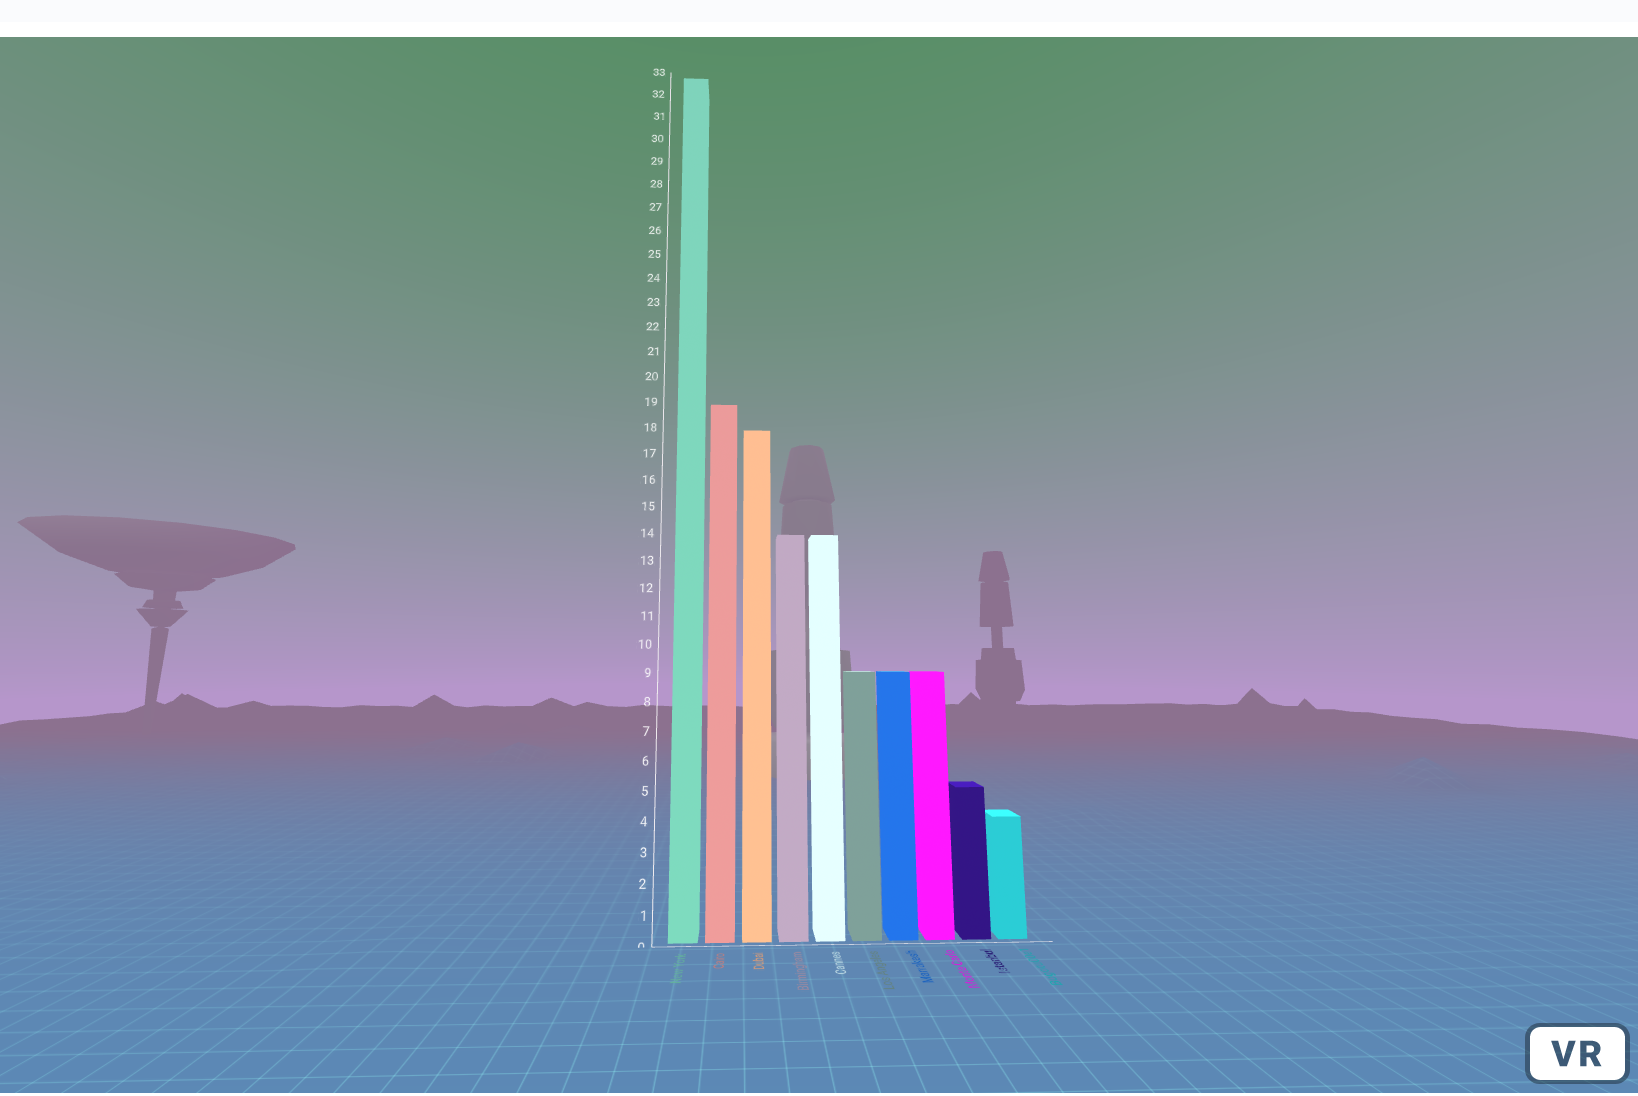
\includegraphics[width=12cm, keepaspectratio]{img/development/visualizacion-bars-use.png}
  \caption{Resultado de Visualización VR Vertical Bars}
  \label{fig:visualizacionbarsuse}
\end{figure}

Una vez lo obtengamos como deseamos, lo guardamos de la misma manera que en la anterior visualización.
El siguiente paso es crear la visualización \textit{VR Vertical Bar 3D} de la misma forma que las anteriores. En este tipo de de gráfica, trabajamos con dos claves para un solo valor. Por ejemplo, para este caso necesitamos que nos diferencie por sexos la clientela de las ciudades con menos ventas; por tanto trabajaremos con las 2 claves que son: por sexo y por ciudad; y un valor: el número de ventas.

Sabiendo esto debemos crear dos buckets en el editor:

\begin{figure}[H]
  \centering
  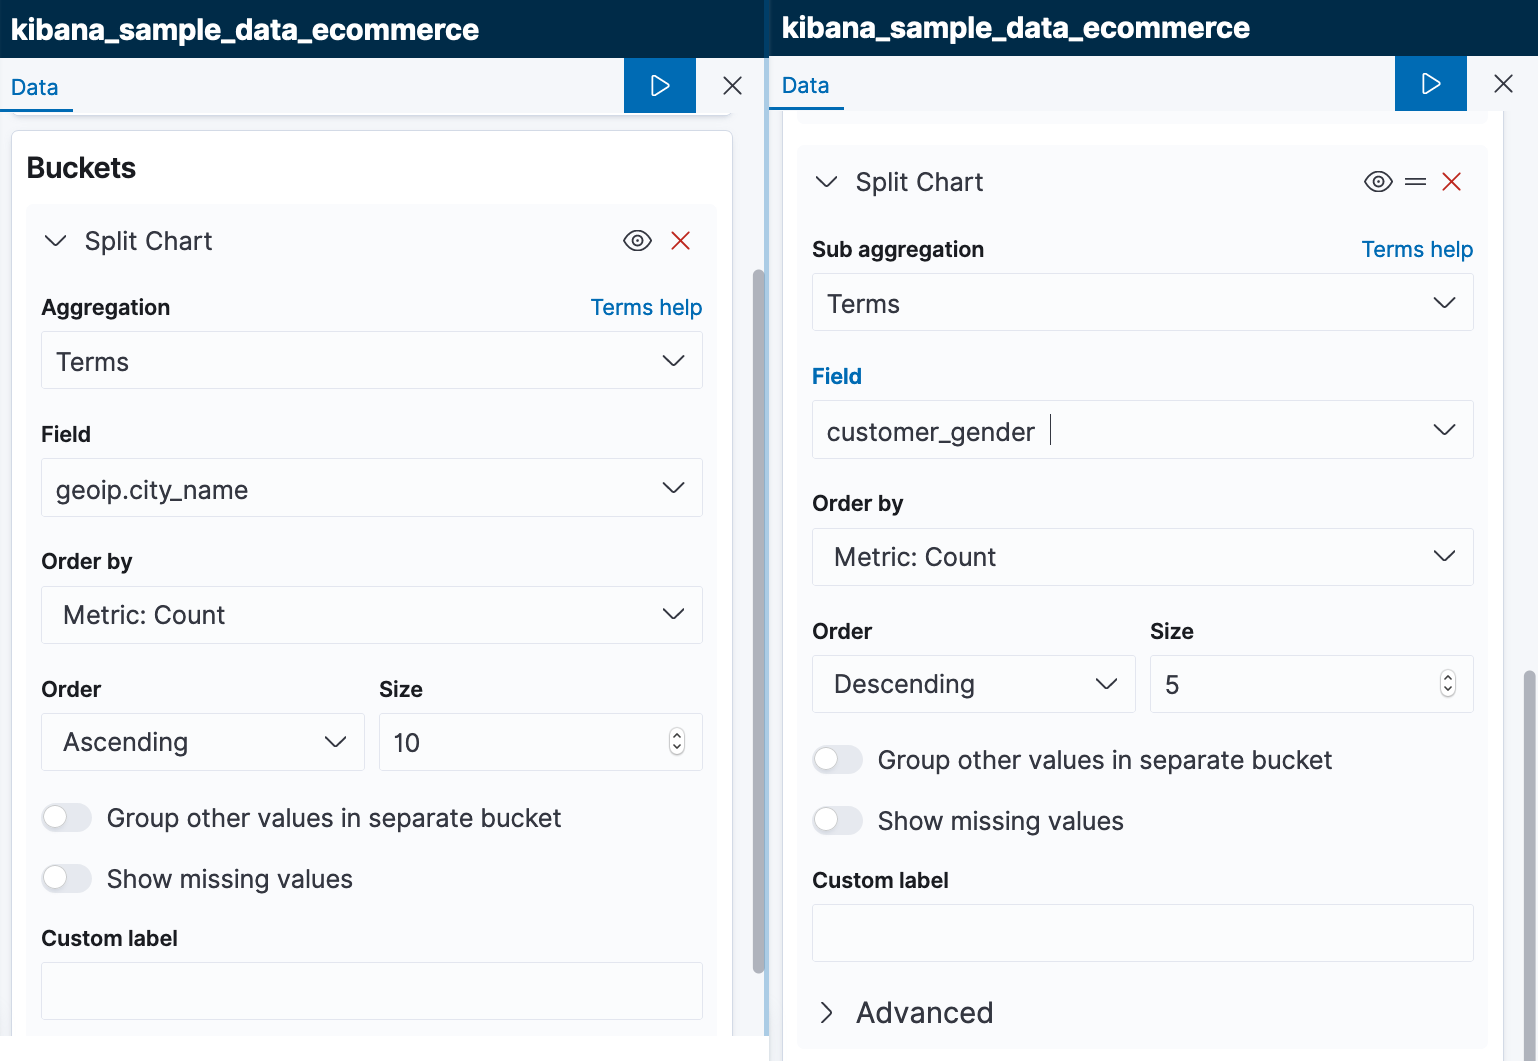
\includegraphics[width=8cm, keepaspectratio]{img/development/editor-3dbars.png}
  \caption{Editor para Visualización VR Vertical Bars 3D}
  \label{fig:editor3dbar}
\end{figure}

Como se ve en la imágenes, en el primer bucket queremos que nos lo clasifique por ciudades y en el siguiente que, a mayores, nos lo clasifique por género. Obteniendo la siguiente visualización.

\begin{figure}[H]
  \centering
  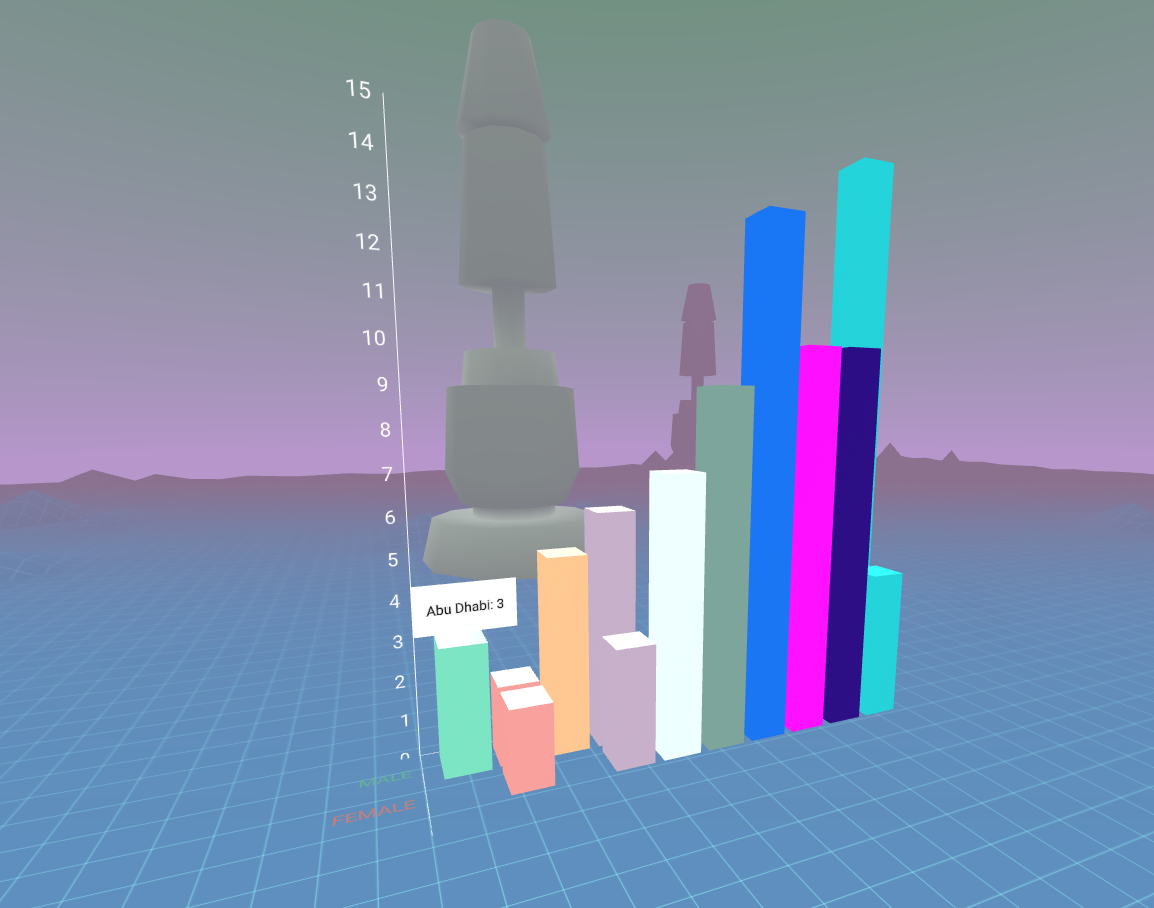
\includegraphics[width=9cm, keepaspectratio]{img/development/visualizacion-3d-bar-use.png}
  \caption{Resultado de Visualización VR Vertical Bars 3D}
  \label{fig:visualizacion3dbar}
\end{figure}

Al igual que con las anteriores, lo guardamos para poder añadirlo más adelante en la dashboard.

Ahora pasamos a crear la última de las visualizaciones. Creamos una visualización \textit{VR Bubble} y la creamos a partir de los siguiente parámetros en el editor.

\begin{figure}[H]
  \centering
  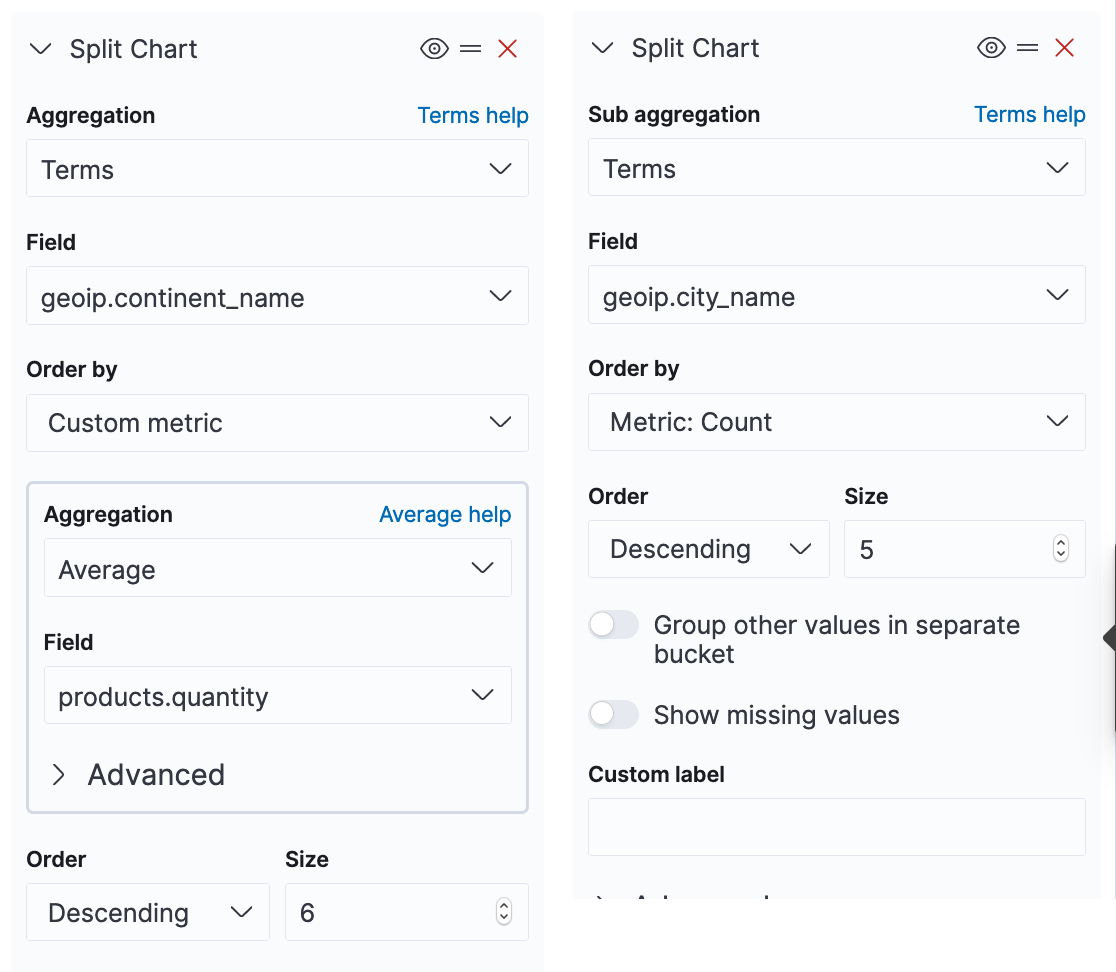
\includegraphics[width=7cm, keepaspectratio]{img/development/editor-bubbles.png}
  \caption{Editor para Visualización VR Bubbles}
  \label{fig:editorbubbles}
\end{figure}

En esta ocasión trabajamos con dos claves y dos valores que son representados por el radio y la altura de la burbuja respectivamentes.

En el editor de la izquierda vemos que queremos que nos muestre las ciudades con más ventas ordenadas de mayor a menor. Y en el editor de la derecha que nos muestre los continentes ordenados según la media de ventas.

Y obtenemos la visualización resultante que la guardaremos de la misma forma que las anteriores.

\begin{figure}[H]
  \centering
  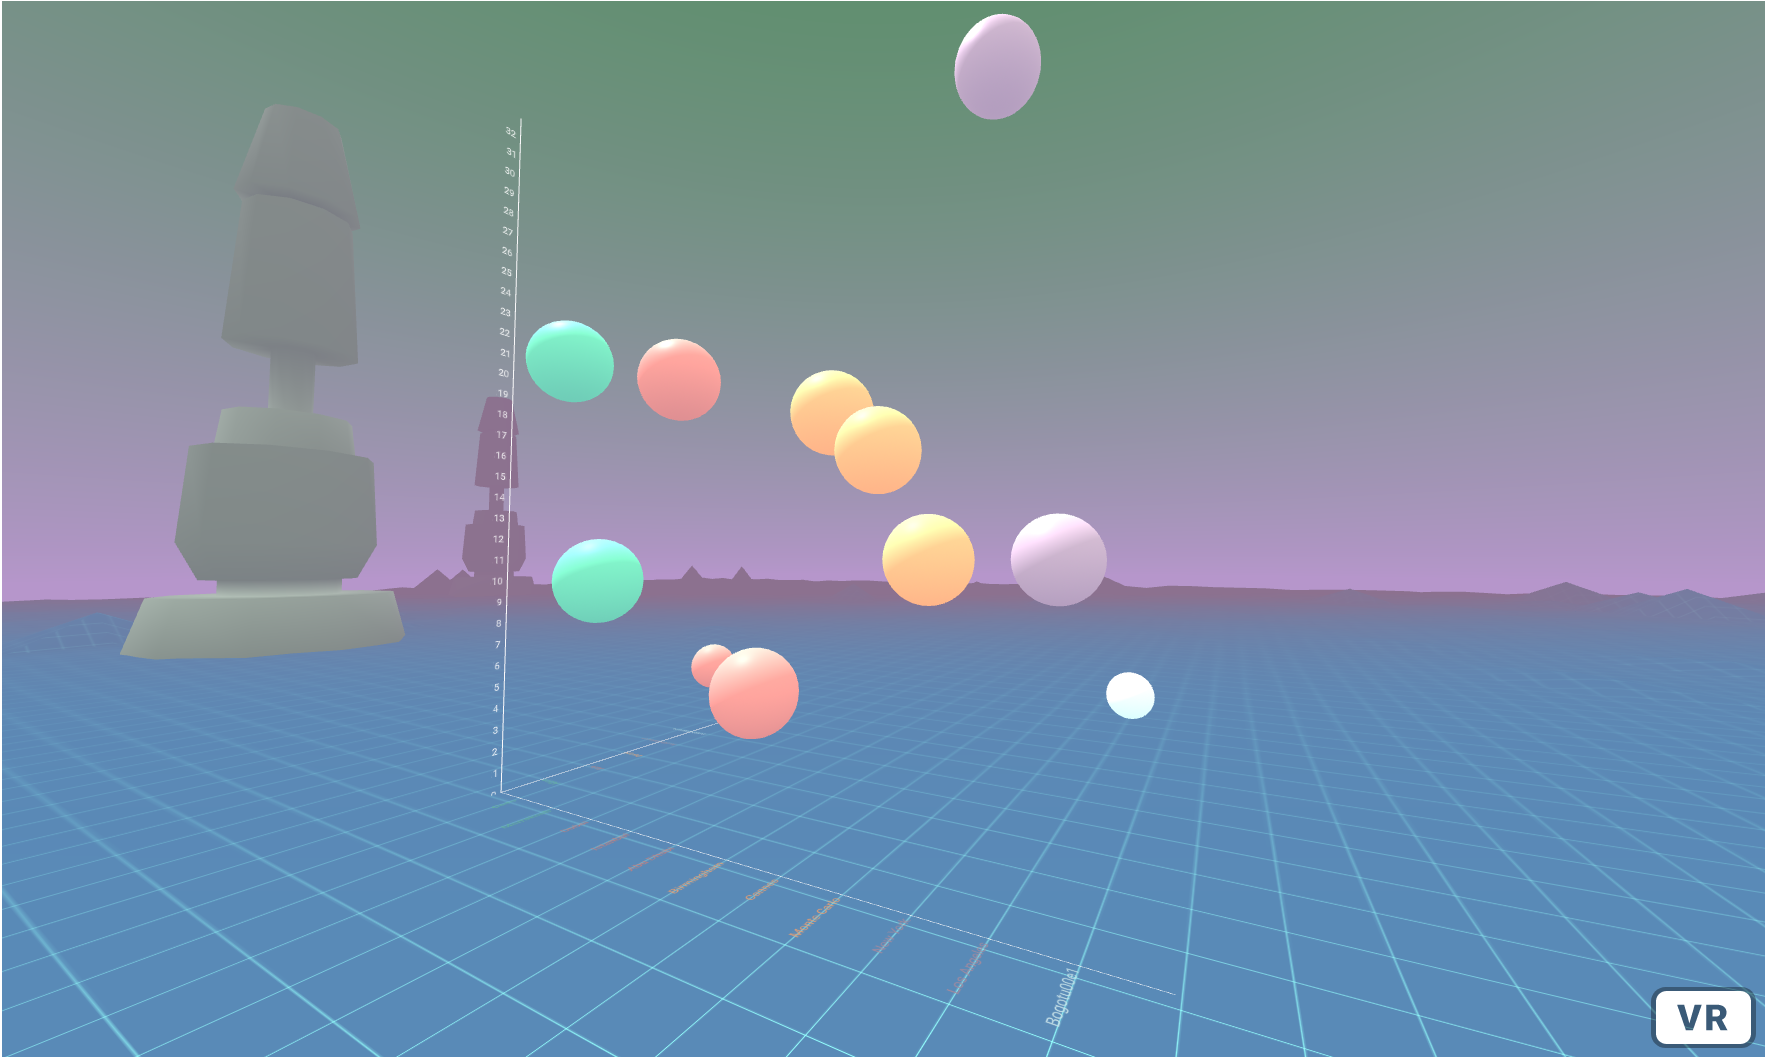
\includegraphics[width=9cm, keepaspectratio]{img/development/visualizacion-bubble-use.png}
  \caption{Resultado de Visualización VR Bubbles}
  \label{fig:visualizacionbubbles}
\end{figure}

En general, el funcionamiento de la creación de las gráficas no difiere mucho de las gráficas predeterminadas de Kibana, por lo que cualquier usuario que tenga conocimientos de Kibana no le será complicado manejar este plugin.

Ahora que ya tenemos todos los tipos de visualizaciones creadas, pasamos a añadirlas a la dashboard. Esta parte se ejecuta de la misma manera que se haría normalmente en Kibana.

Accedemos a la pestaña \textit{Dashboard} y le damos a \textit{Create Dashboard}. Aquí nos encontramos con un lienzo en blanco donde iremos añadiendo cada una de nuestras visualizaciones acomodandolas según las preferencias del usuario.

Un ejemplo de Dashboard puede ser como la siguiente:


\begin{figure}[H]
  \centering
  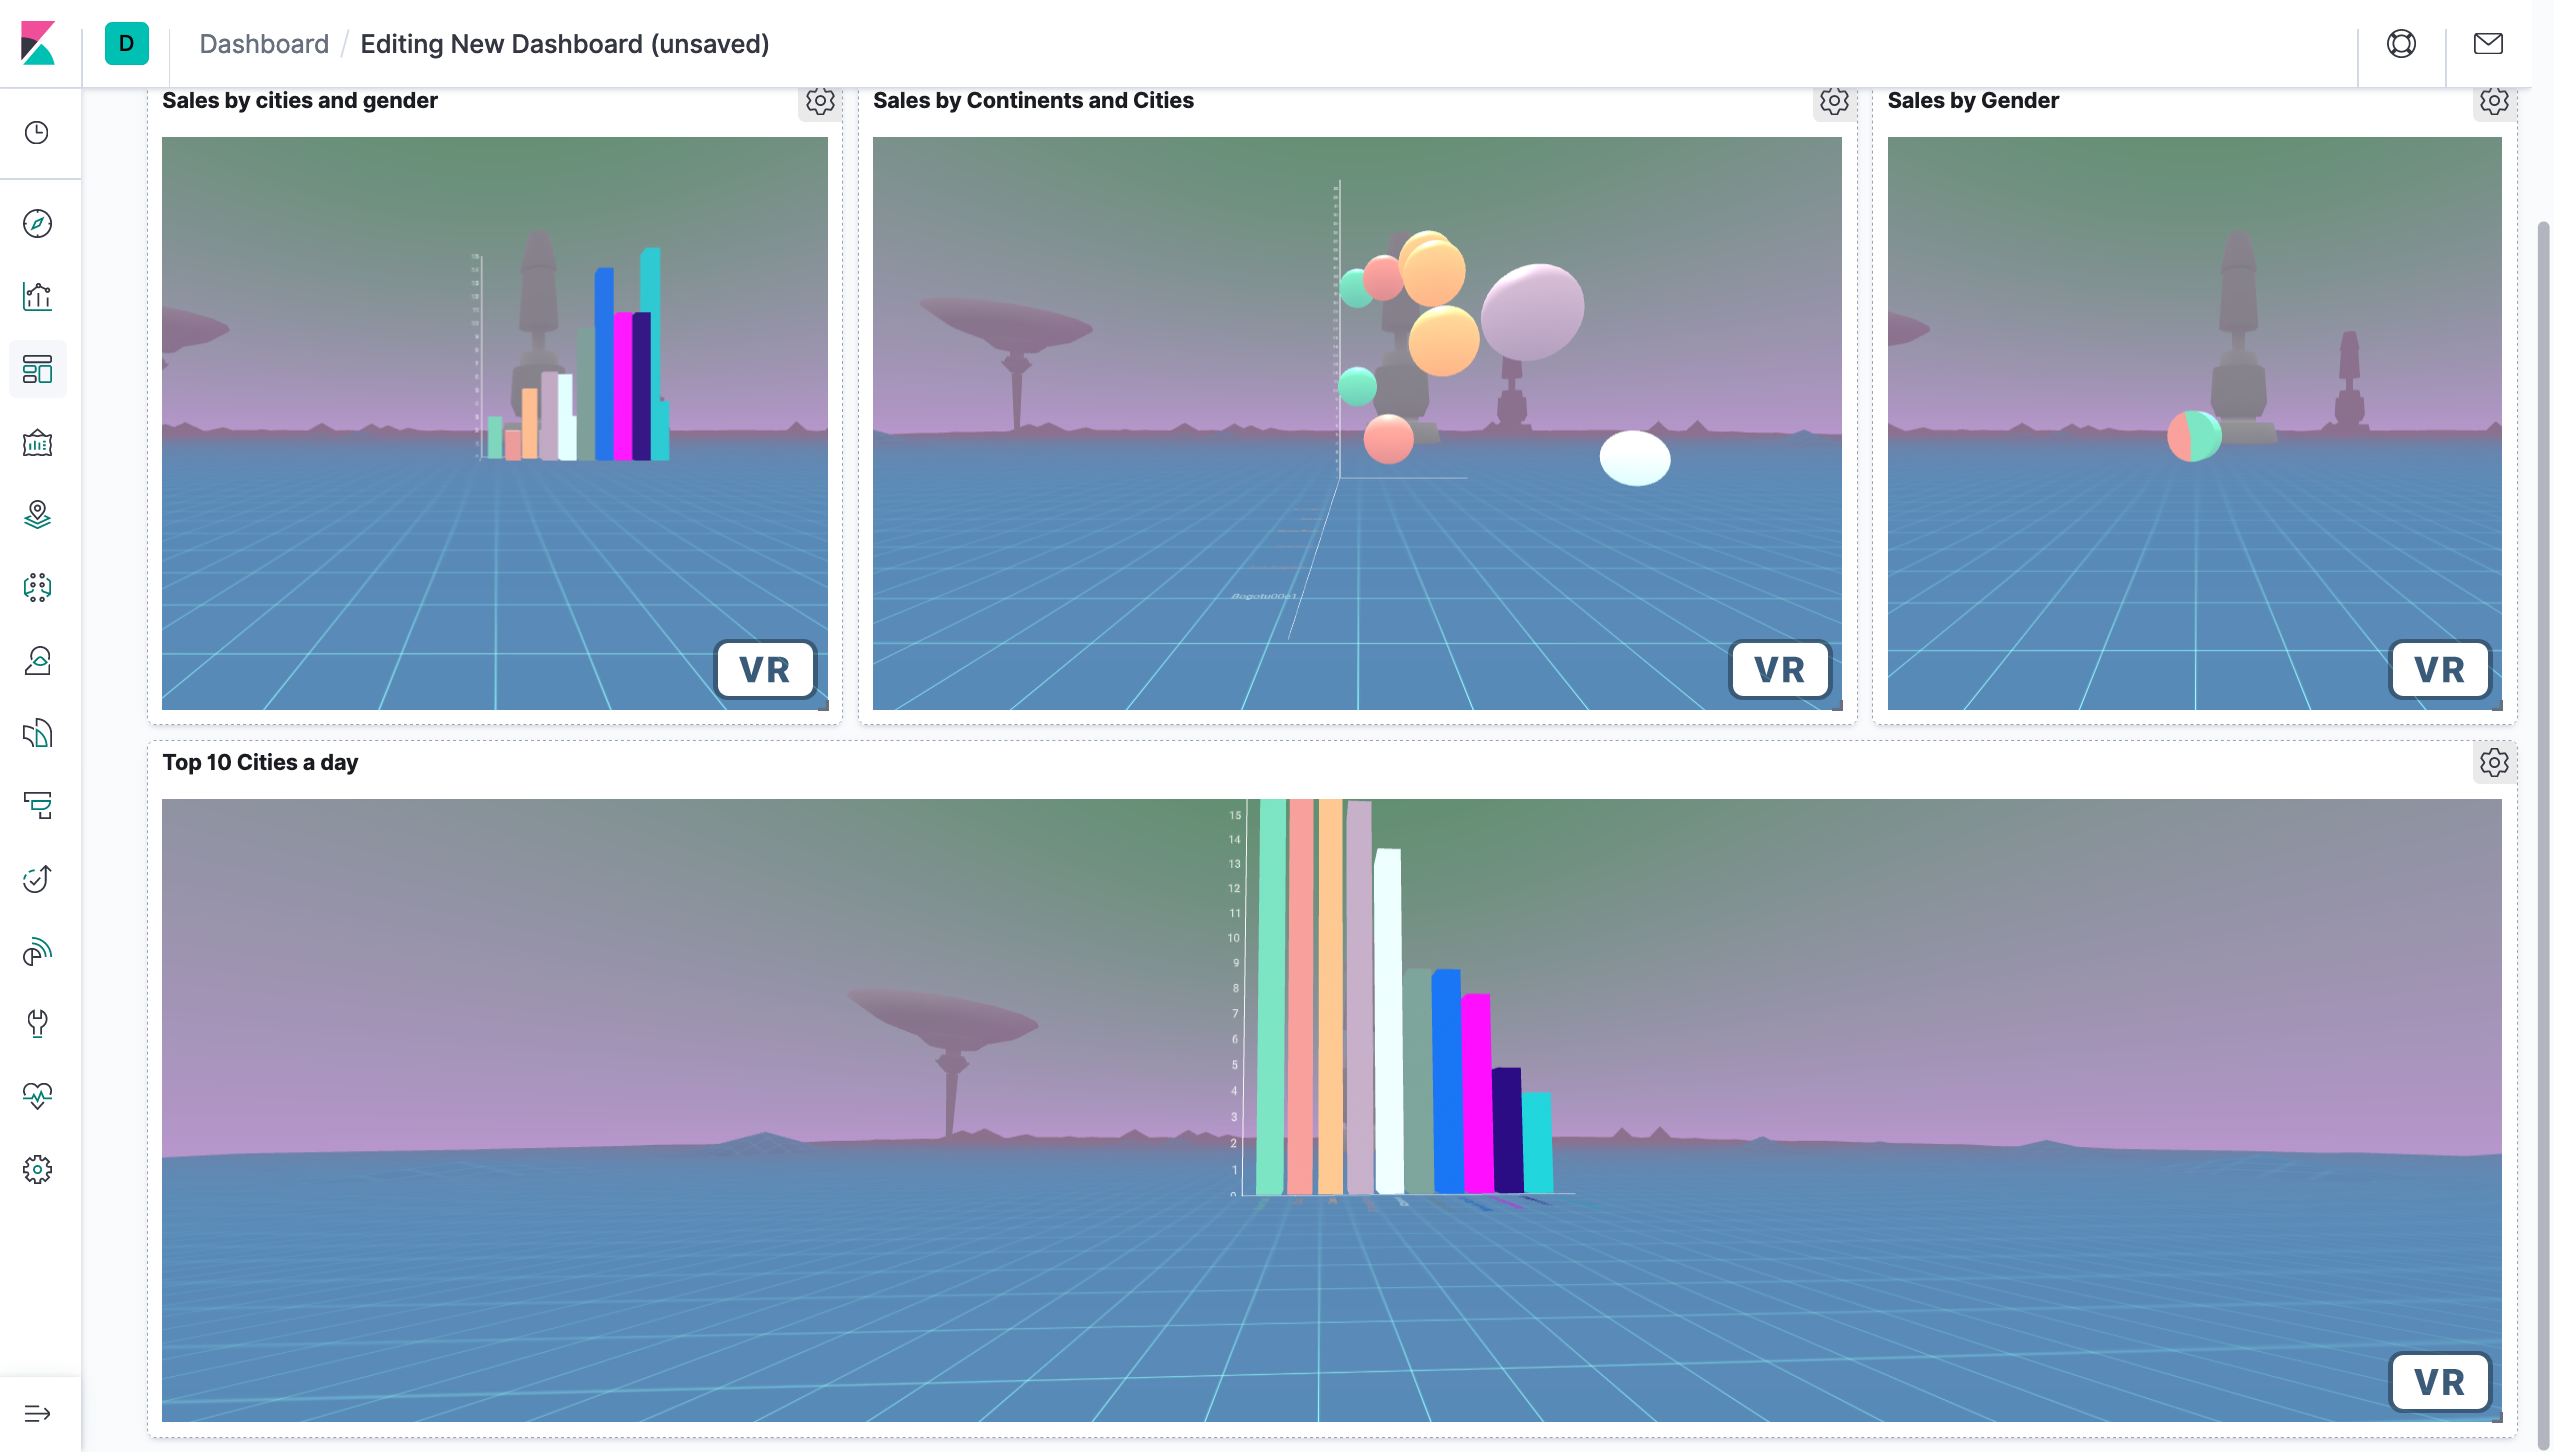
\includegraphics[width=12cm, keepaspectratio]{img/development/dashboard-use.png}
  \caption{Resultado de la dashboard con las visualizaciones VR}
  \label{fig:dashboardresultado}
\end{figure}

Uno de los detalles a mencionar es que si colocas varias visualizaciones de A-Frame en la misma dashboard, cuando modificas la posición de una, todas las demás también lo harán. También, podrás tener una experiencia de inmersión en cada una de ellas de forma individual.


%%%%%%%%%%%%%%%%%%%%%%%%%%%%%%%%%%%%%%%%%%%%%%%%%%%%%%%%%%%%%%%%%
% CONCLUSIONES %
%%%%%%%%%%%%%%%%%%%%%%%%%%%%%%%%%%%%%%%%%%%%%%%%%%%%%%%%%%%%%%%%%

\cleardoublepage
\chapter{Conclusiones}
\label{sec:conclusiones} 

\section{Consecución de objetivos}
\label{sec:objetivoscumplidos}

El objetivo principal de este proyecto era la creación de una biblioteca de visualizaciones dentro de un entorno de Realidad Virtual para Kibana. Si vemos los resultados del proyecto, podemos decir que hemos cumplido satisfactoriamente este objetivo.

Por otra parte, analizaremos si se han completado todos y cada uno de los objetivos específicos que nos propusimos:

Se ha creado un plugin para Kibana que crea visualizaciones, a partir de datos obtenidos de Elasticsearch, dentro de un entorno VR. Para realizar este desarrollo se ha utilizado la biblioteca BabiaXR.

Centrándonos en el plugin, este cuenta con varios tipos de visualizaciones que se asemejan a las visualizaciones predeterminadas de Kibana. Además, se pueden añadir a una dashboard que vienen integrada dentro del propio Kibana.

La construcción de cada visualización está pensada para que cualquier usuario que conozca Kibana no necesite aprender a utilizarla, ya que han sido desarrolladas replicando el funcionamiento de las predeterminadas.

Actualmente, no he encontrado otras herramientas que permitan elegir si se desea representar datos en 2D o en 3D con la posibilidad de inmersión en VR. Todo lo que he encontrado se centra solo en un único modo de representación.

Por último nos centramos en la distribución. A día de hoy se ha añadido el plugin actualizado en su última versión, compatible con la versión 7.6 de Kibana, en Github y se ha procedido a incluirla dentro de la comunidad para que puedan colaborar en futuras mejoras para este proyecto. Además, también se ha creado una versión para Kibana 7.4.2 que es compatible para usarlo con la última versión de Opendistro for Elasticsearch. Estos instaladores se han preparado para que la instalación sea lo más sencilla posible.


En conclusión, podemos decir que se ha cumplido con todos lo objetivos propuestos. Sin dejar de lado el único objetivo que no hemos mencionado, pero que es más importante que todo lo anterior: el haber obtenido todos los conocimientos adquiridos en este proceso.


\section{Aplicación de lo aprendido}
\label{sec:aprendido}

Para llevar a cabo este proyecto, se ha tenido que partir de unos conocimientos básicos adquiridos durante el grado. La mayor parte de este proyecto se ha desarrollado usando lenguajes centrado en la programación Web, tales como HTML, CSS y Javascript. 

Estos lenguajes ya se conocían anteriormente gracias a asignaturas como \textit{Construcción de servicios y aplicaciones audiovisuales en internet} o \textit{Laboratorio de Tecnologías audiovisuales en la web}. Sin olvidarnos que todas la bases de la lógica y la programación adquiridas en las asignaturas de \textit{Informática I} e \textit{Informática II}. 

Otro de los puntos clave era conocer el concepto de cliente-servidor, ya que Kibana hace la función de cliente haciendo peticiones; y Elasticsearch la función servidor facilitando los datos pedidos. Estos conceptos los aprendimos en \textit{Informatica II} y los profundizamos en \textit{Protocolos para la transmisión de audio y video en internet}. 

Por último, mencionar que también se poseían unos conocimientos en relación a la creación de gráficos en 3D gracias a la asignatura \textit{Gráficos y visualizaciones en 3D}.

\section{Lecciones aprendidas}
\label{sec:lecciones}

Durante todo el proceso de creación de este proyecto he adquirido los siguientes conocimientos:

\begin{itemize}
    \item Aumentar mis conocimientos en cuanto a lenguajes para la programación web tanto en la parte back-end como front-end.
    \item Aprender el funcionamiento de la herramienta Kibana y cómo crear plugins de visualización para ésta. Esto engloba también la creación de un entorno de desarrollo y lanzar servidores de prueba durante el desarrollo.
    \item Trabajar usando una metodología para el desarrollo ágil de proyectos.
    \item Aprender a usar nuevas tecnologías para la creación de elementos en entornos de Realidad Virtual como es el caso de A-Frame.
    \item Trabajar usando datos reales obtenidos de Elasticsearch.
    \item A usar \LaTeX  para la redacción de esta memoria. 
    \item Mejorar el uso de Git para gestionar proyectos alojados en Github.
\end{itemize}


\section{Futuros Trabajos}
\label{sec:futuro}

 Este proyecto no se puede dar por terminado, pues todavía se puede mejorar en muchos sentidos. Estas son algunas de las mejoras que se podrían llevar a cabo:
 
 \begin{itemize}
     \item Añadir más opciones de customización tales como: cambiar los colores de las gráficas, añadir leyenda, posiciones de las gráficas al gusto, etc.
     \item Añadir más tipos de visualizaciones.
     \item Mejorar el escenario en función de las preferencias del usuario.
     \item Escalado de las gráficas, pues ahora mismo no permite esta posibilidad.
     \item Crear una dashboard que sea un entorno de Realidad Virtual y que sus visualizaciones sean elementos dentro de dicho entorno.
     \item Añadir más versiones para que puedan usarse en diferentes versiones de Kibana.
     \item Creación nuevos plugins.
 \end{itemize}
 
 Actualmente estoy colaborando para mejorar la biblioteca de BabiaXR, añadiendo muchas de estas mejoras que se han comentado para, más adelante, integrarlas en este proyecto. Es de gran ayuda ya que algunas de estas mejoras no se podían realizar por culpa de las propias limitaciones de la biblioteca.


%%%%%%%%%%%%%%%%%%%%%%%%%%%%%%%%%%%%%%%%%%%%%%%%%%%%%%%%%%%%%%%%%%%%%%%%%%%%%%%%
%%%%%%%%%%%%%%%%%%%%%%%%%%%%%%%%%%%%%%%%%%%%%%%%%%%%%%%%%%%%%%%%%%%%%%%%%%%%%%%%
% APENDICE(S) %
%%%%%%%%%%%%%%%%%%%%%%%%%%%%%%%%%%%%%%%%%%%%%%%%%%%%%%%%%%%%%%%%%%%%%%%%%%%%%%%%
%\cleardoublepage
%\appendix
%\chapter{Código del proyecto}
%\label{sec:apendice}
%\section{Código del plugin}

%\subsection{package.json}
%\label{sec:codepackage}
%\lstinputlisting[language=Json]{code/final-package.json}

%\subsection{index.js}
%\label{sec:codeindex}
%\lstinputlisting[language=Javascript]{code/final-index.js}

%\subsection{kbn\_aframe.js}
%\label{sec:codekbnaframe}
%\lstinputlisting[language=Javascript]{code/final-kbn-aframe.js}

%\subsection{pie.js}
%\label{sec:codepie}
%\lstinputlisting[language=Javascript]{code/final-pie.js}

%\subsection{simple\_bar.js}
%\label{sec:codesimplebar}
%\lstinputlisting[language=Javascript]{code/final-simple-bar.js}

%\subsection{3d\_bar.js}
%\label{sec:code3dbar}
%\lstinputlisting[language=Javascript]{code/final-3d-bar.js}

%\subsection{bubble.js}
%\label{sec:codebubble}
%\lstinputlisting[language=Javascript]{code/final-bubble.js}

%\subsection{kbn\_aframe\_controller.js}
%\label{sec:codecontroller}
%\lstinputlisting[language=Javascript]{code/final-kbn-aframe-controller.js}

%\subsection{metrics.js}
%\label{sec:codemetrics}
%\lstinputlisting[language=Javascript]{code/final-metrics.js}

%\subsection{a\_scene.js}
%\label{sec:codeascene}
%\lstinputlisting[language=Javascript]{code/final-a-scene.js}

%\subsection{a\_controls.js}
%\label{sec:codeacontrols}
%\lstinputlisting[language=Javascript]{code/final-a-controls.js}

%\subsection{a\_charts.js}
%\label{sec:codeacharts}
%\lstinputlisting[language=Javascript]{code/final-a-charts.js}

%\subsection{kbn\_aframe.less}
%\label{sec:codestyle}
%\lstinputlisting[language=Javascript]{code/final-kbn-aframe.less}


%%%%%%%%%%%%%%%%%%%%%%%%%%%%%%%%%%%%%%%%%%%%%%%%%%%%%%%%%%%%%%%%%%%%%%%%%%%%%%%%
%%%%%%%%%%%%%%%%%%%%%%%%%%%%%%%%%%%%%%%%%%%%%%%%%%%%%%%%%%%%%%%%%%%%%%%%%%%%%%%%
% BIBLIOGRAFIA %
%%%%%%%%%%%%%%%%%%%%%%%%%%%%%%%%%%%%%%%%%%%%%%%%%%%%%%%%%%%%%%%%%%%%%%%%%%%%%%%%
% para que funcione la bibliografia hay que meter las referencias con \cite{blokehead:scrum} sino no aparecera.
\cleardoublepage
\label{sec:bibliografia}
% Las siguientes dos instrucciones es todo lo que necesitas
% para incluir las citas en la memoria
\bibliographystyle{abbrv}
\bibliography{memoria}  % memoria.bib es el nombre del fichero que contiene
% las referencias bibliográficas. Abre ese fichero y mira el formato que tiene,
% que se conoce como BibTeX. Hay muchos sitios que exportan referencias en
% formato BibTeX. Prueba a buscar en http://scholar.google.com por referencias
% y verás que lo puedes hacer de manera sencilla.
% Más información: 
% http://texblog.org/2014/04/22/using-google-scholar-to-download-bibtex-citations/



% Esto va al final de todo.
\end{document}